\documentclass{article}

\usepackage{arxiv}
\usepackage[utf8]{inputenc}
\usepackage[T1]{fontenc}
\usepackage{hyperref}
\usepackage{url}
\usepackage{xurl}
\usepackage{booktabs}
\usepackage{amsmath,amsfonts,amssymb}
\usepackage{nicefrac}
\usepackage{microtype}
\usepackage{graphicx}
\usepackage{caption}
\usepackage{subcaption}
\usepackage{enumitem}
\usepackage{tabularx}
\usepackage[numbers,sort&compress]{natbib}
\usepackage{doi}
\usepackage{xcolor}
\usepackage{tikz}
\usetikzlibrary{arrows.meta,positioning,fit,backgrounds,calc}
\usepackage[group-separator={,},group-minimum-digits=4,mode=text]{siunitx}
\usepackage[capitalise,noabbrev]{cleveref}
\usepackage[section]{placeins}

% Okabe-Ito colours, identical to figure_code/paper_style.py (validated for
% colour-vision deficiency on white). Used by TikZ figures in the paper.
\definecolor{okblue}{HTML}{0072B2}
\definecolor{okverm}{HTML}{D55E00}
\definecolor{okgreen}{HTML}{009E73}
\definecolor{okorange}{HTML}{E69F00}
\definecolor{okpurple}{HTML}{CC79A7}
\definecolor{oksky}{HTML}{56B4E9}
\definecolor{ink}{HTML}{1A1A1A}
\definecolor{inktwo}{HTML}{4D4D4D}
\definecolor{rule}{HTML}{BDBDBD}
\definecolor{okyellow}{HTML}{F0E442}

% Event facts that are not computed from data. Each has a source in
% writing/claim_ledger.md; change them only together with the ledger.
\newcommand{\eventname}{HackAlem~AI}
\newcommand{\eventdate}{23~September 2026}          % ledger #1 (hackalem.ai)
\newcommand{\eventwindow}{13:00--18:00}             % ledger #8 (inferred; official source todo)
\newcommand{\astanatz}{UTC$+$5}                     % Kazakhstan time zone
\newcommand{\eventhours}{five}                      % press reports of a five-hour window
\newcommand{\seats}{\num{2500}}                     % ledger #4 (hackalem.ai)
\newcommand{\applications}{\num{6586}}              % ledger #4 (Qumash.kz, Ulys Media)
\newcommand{\countries}{21}                         % ledger #5 (Kazinform, Astana Times)
\newcommand{\teamsizemax}{three}                    % ledger #2 (hackalem.ai)
\newcommand{\agemin}{18}                             % ledger #28 (hackalem.ai eligibility, read 29 Sep 2026)
\newcommand{\gradmonths}{12}                         % ledger #28 (hackalem.ai: full-time IT study in the last 12 months)
\newcommand{\prevrecord}{\num{2089}}                % ledger #6 (Astana Times)
\newcommand{\awardsdate}{23~October 2026}           % ledger #15 (hackalem.ai timeline, read 29 Sep 2026)
\newcommand{\datacollected}{24~September 2026}      % our collection date
\newcommand{\ghorg}{\texttt{BAITC-Hacks}}
\newcommand{\eventstart}{13:00}
\newcommand{\deadline}{18:00}
\newcommand{\dayend}{19:00}
\newcommand{\batchday}{22~September}
\newcommand{\batchwindow}{18:00--20:00}
\newcommand{\sepone}{1~September}
\newcommand{\seponefour}{14~September}
\newcommand{\sepfifteen}{15~September}
\newcommand{\septwentyone}{21~September}
\newcommand{\prizes}{US\$1.1~million}                % ledger (hackalem.ai): prizes and technology resources
\newcommand{\pending}[1]{\textcolor{okverm}{[pending: #1]}}
\newcommand{\chisq}{\ensuremath{\chi^2}}
\newcommand{\participantsreported}{more than \num{2500}}  % ledger #17 (Astana Times: "More than 2,500 participants from 21 countries and 129 universities")
\newcommand{\universities}{129}                       % ledger #17 (Astana Times)
\newcommand{\sepseventeen}{17~September}
\newcommand{\reviewperiod}{24~September--13~October}  % ledger #18 (hackalem.ai timeline, read 29 Sep 2026)
\newcommand{\demoday}{16~October}                    % ledger #18 (hackalem.ai: finalists present, winners announced; read 29 Sep 2026)
\newcommand{\versiondate}{3~October 2026}
\newcommand{\disclosuredate}{28~September 2026}           % ledger #21 (sent e-mail to team@baitc.org; .eml kept privately)
\newcommand{\zenodorelease}{\doi{10.5281/zenodo.23091476}}  % Zenodo record 23091476, release v1.0.4 (version DOI), published 2026-10-02
\newcommand{\zenodoversion}{v1.0.4}

% Method constants, identical to the values in the code named on each line.
\newcommand{\templatesecs}{\num{120}~s}              % src/build_repo_table.py is_template; checks/recompute_core.py
\newcommand{\thrcyr}{50\%}                            % src/readme_features.py language()
\newcommand{\thrkaz}{3\%}                             % src/readme_features.py language()
\newcommand{\thrlat}{80\%}                            % src/readme_features.py language()
\newcommand{\minletters}{20}                          % src/readme_features.py: fewer letters -> too short
\newcommand{\entropythr}{3.5}                         % src/secrets_precision.py classify()
\newcommand{\gitleaksversion}{8.30.1}                 % tools/gitleaks (checksum-verified release)
\newcommand{\nullruns}{20}                            % analysis/run_analysis.py null model for silhouettes
\newcommand{\evenshare}{20\%}                         % one hour of five: an even spread
\newcommand{\majorityshare}{50\%}
\newcommand{\equivlo}{0.5}                            % prereg/jury_preregistration.md, Section 5.4
\newcommand{\equivhi}{2.0}
\newcommand{\epsq}{\ensuremath{\varepsilon^2}}
\newcommand{\lasthourstart}{17:00}                    % start of the last hour of the event window
\newcommand{\epsqformula}{\ensuremath{\varepsilon^2 = H/(n-1)}}  % Kruskal-Wallis effect size (analysis/run_analysis.py)
\newcommand{\trackminscore}{two}                      % src/hackalem_repo_scan.py MIN_SCORE
\newcommand{\haldane}{0.5}                           % analysis/run_analysis.py self_report assoc: Haldane-Anscombe correction
\newcommand{\solruns}{\num{999}}                      % analysis/run_analysis.py SOL_RUNS (label shuffles)
\newcommand{\codebookdate}{28~September 2026}         % data/llm_codebook/responses.jsonl time_utc
\newcommand{\readmechars}{\num{2500}}                 % src/llm_codebook.py README_CHARS
\newcommand{\maxpaths}{\num{40}}                      % src/llm_codebook.py MAX_PATHS
\newcommand{\minbytes}{\num{200}}                    % src/extract_solutions.py MIN_BYTES

% Numbers quoted from the literature, each with its source (abstract read, see literature/notes).
\newcommand{\robbesrate}{22.20--28.66\%}              % Robbes et al., TOSEM 2026, abstract
\newcommand{\robbesprojects}{\num{128018}}            % Robbes et al., TOSEM 2026, abstract
\newcommand{\swechatshare}{41\%}                      % Baumann et al. 2026 (SWE-chat), abstract
\newcommand{\gitleaksprecision}{46\%}                 % Basak et al., ESEM 2023, abstract
\newcommand{\gitleaksrecall}{88\%}                    % Basak et al., ESEM 2023, abstract
\newcommand{\hackrepsize}{\num{100356}}               % Halmans et al., MSR 2026 (HackRep), abstract
\newcommand{\devpostprojects}{\num{22183}}            % Imam et al. 2021; Mahmoud et al. 2022, abstracts
\newcommand{\hackcodeshare}{9.14\%}                   % Imam et al. 2021, abstract: blobs created during hackathons

% Generated by analysis/make_numbers.py. Do not edit by hand.
% Source: arxiv_paper_all/analysis/facts_paper.json
\newcommand{\NLiteratureScreened}{\num{66}}
\newcommand{\NLiteratureSearches}{\num{122}}
\newcommand{\NRqFourEnvExampleHi}{\num{76.8}}
\newcommand{\NRqFourEnvExampleLo}{\num{71.5}}
\newcommand{\NRqFourEnvExampleN}{\num{785}}
\newcommand{\NRqFourEnvExampleOf}{\num{1057}}
\newcommand{\NRqFourEnvExamplePct}{\num{74.3}}
\newcommand{\NRqFourEnvFileCommittedHi}{\num{4.5}}
\newcommand{\NRqFourEnvFileCommittedLo}{\num{2.3}}
\newcommand{\NRqFourEnvFileCommittedN}{\num{34}}
\newcommand{\NRqFourEnvFileCommittedOf}{\num{1057}}
\newcommand{\NRqFourEnvFileCommittedPct}{\num{3.2}}
\newcommand{\NRqFourGenericDataFilesPct}{\num{93.5}}
\newcommand{\NRqFourGenericFindings}{\num{4597}}
\newcommand{\NRqFourGenericRepos}{\num{131}}
\newcommand{\NRqFourGitignoreAssocExampleAmongIgnore}{\num{83.6}}
\newcommand{\NRqFourGitignoreAssocExampleAmongNoIgnore}{\num{26.6}}
\newcommand{\NRqFourGitignoreAssocIgnoreAmongLlm}{\num{90.9}}
\newcommand{\NRqFourGitignoreAssocIgnoreAmongNoLlm}{\num{63.9}}
\newcommand{\NRqFourGitignoreAssocMhHi}{\num{2.37}}
\newcommand{\NRqFourGitignoreAssocMhLo}{\num{0.45}}
\newcommand{\NRqFourGitignoreAssocMhOr}{\num{1.03}}
\newcommand{\NRqFourGitignoreAssocMhP}{= 0.948}
\newcommand{\NRqFourGitignoreAssocP}{= 0.287}
\newcommand{\NRqFourGitignoreAssocV}{\num{0.03}}
\newcommand{\NRqFourGitignoreAssocWithIgnore}{\num{6.1}}
\newcommand{\NRqFourGitignoreAssocWithoutIgnore}{\num{4.0}}
\newcommand{\NRqFourGitignoreCoversEnvHi}{\num{85.7}}
\newcommand{\NRqFourGitignoreCoversEnvLo}{\num{81.3}}
\newcommand{\NRqFourGitignoreCoversEnvN}{\num{884}}
\newcommand{\NRqFourGitignoreCoversEnvOf}{\num{1057}}
\newcommand{\NRqFourGitignoreCoversEnvPct}{\num{83.6}}
\newcommand{\NRqFourKeyByExampleWithExample}{\num{6.5}}
\newcommand{\NRqFourKeyByExampleWithoutExample}{\num{3.7}}
\newcommand{\NRqFourKeyCommitsBaselineSignedSameReposHi}{\num{10.6}}
\newcommand{\NRqFourKeyCommitsBaselineSignedSameReposLo}{\num{7.7}}
\newcommand{\NRqFourKeyCommitsBaselineSignedSameReposN}{\num{138}}
\newcommand{\NRqFourKeyCommitsBaselineSignedSameReposOf}{\num{1528}}
\newcommand{\NRqFourKeyCommitsBaselineSignedSameReposPct}{\num{9.0}}
\newcommand{\NRqFourKeyCommitsFindings}{\num{77}}
\newcommand{\NRqFourKeyCommitsMatched}{\num{73}}
\newcommand{\NRqFourKeyCommitsSignedByKindClaude}{\num{2}}
\newcommand{\NRqFourKeyCommitsSignedByKindCodex}{\num{2}}
\newcommand{\NRqFourKeyCommitsSignedByKindCursor}{\num{1}}
\newcommand{\NRqFourKeyCommitsSignedHi}{\num{15.1}}
\newcommand{\NRqFourKeyCommitsSignedLo}{\num{3.0}}
\newcommand{\NRqFourKeyCommitsSignedN}{\num{5}}
\newcommand{\NRqFourKeyCommitsSignedOf}{\num{73}}
\newcommand{\NRqFourKeyCommitsSignedPct}{\num{6.8}}
\newcommand{\NRqFourNodeModulesCommittedHi}{\num{1.4}}
\newcommand{\NRqFourNodeModulesCommittedLo}{\num{0.3}}
\newcommand{\NRqFourNodeModulesCommittedN}{\num{7}}
\newcommand{\NRqFourNodeModulesCommittedOf}{\num{1057}}
\newcommand{\NRqFourNodeModulesCommittedPct}{\num{0.7}}
\newcommand{\NRqFourOpenaiFilesEnv}{\num{27}}
\newcommand{\NRqFourOpenaiFilesEnvExample}{\num{32}}
\newcommand{\NRqFourOpenaiFilesEnvOther}{\num{3}}
\newcommand{\NRqFourOpenaiFilesSourceOrText}{\num{15}}
\newcommand{\NRqFourOpenaiFinalHi}{\num{4.0}}
\newcommand{\NRqFourOpenaiFinalLo}{\num{2.0}}
\newcommand{\NRqFourOpenaiFinalN}{\num{30}}
\newcommand{\NRqFourOpenaiFinalOf}{\num{1057}}
\newcommand{\NRqFourOpenaiFinalPct}{\num{2.8}}
\newcommand{\NRqFourOpenaiFindings}{\num{77}}
\newcommand{\NRqFourOpenaiHi}{\num{7.3}}
\newcommand{\NRqFourOpenaiInWindowHi}{\num{100.0}}
\newcommand{\NRqFourOpenaiInWindowLo}{\num{95.2}}
\newcommand{\NRqFourOpenaiInWindowN}{\num{77}}
\newcommand{\NRqFourOpenaiInWindowOf}{\num{77}}
\newcommand{\NRqFourOpenaiInWindowPct}{\num{100.0}}
\newcommand{\NRqFourOpenaiLo}{\num{4.5}}
\newcommand{\NRqFourOpenaiN}{\num{61}}
\newcommand{\NRqFourOpenaiOf}{\num{1057}}
\newcommand{\NRqFourOpenaiPct}{\num{5.8}}
\newcommand{\NRqFourProviderFindings}{\num{127}}
\newcommand{\NRqFourProviderPlaceholder}{\num{10}}
\newcommand{\NRqFourProviderPlausible}{\num{117}}
\newcommand{\NRqFourProviderReposNotActive}{\num{0}}
\newcommand{\NRqFourProviderRulesCurlauthheaderFinal}{\num{3}}
\newcommand{\NRqFourProviderRulesCurlauthheaderRepos}{\num{8}}
\newcommand{\NRqFourProviderRulesCurlauthuserFinal}{\num{1}}
\newcommand{\NRqFourProviderRulesCurlauthuserRepos}{\num{2}}
\newcommand{\NRqFourProviderRulesGcpapikeyFinal}{\num{3}}
\newcommand{\NRqFourProviderRulesGcpapikeyRepos}{\num{3}}
\newcommand{\NRqFourProviderRulesJwtFinal}{\num{2}}
\newcommand{\NRqFourProviderRulesJwtRepos}{\num{3}}
\newcommand{\NRqFourProviderRulesOpenaiapikeyFinal}{\num{30}}
\newcommand{\NRqFourProviderRulesOpenaiapikeyRepos}{\num{61}}
\newcommand{\NRqFourProviderRulesStripeaccesstokenFinal}{\num{0}}
\newcommand{\NRqFourProviderRulesStripeaccesstokenRepos}{\num{1}}
\newcommand{\NRqFourProviderRulesTelegrambotapitokenFinal}{\num{0}}
\newcommand{\NRqFourProviderRulesTelegrambotapitokenRepos}{\num{2}}
\newcommand{\NRqFourPycacheCommittedHi}{\num{4.9}}
\newcommand{\NRqFourPycacheCommittedLo}{\num{2.6}}
\newcommand{\NRqFourPycacheCommittedN}{\num{38}}
\newcommand{\NRqFourPycacheCommittedOf}{\num{1057}}
\newcommand{\NRqFourPycacheCommittedPct}{\num{3.6}}
\newcommand{\NRqFourReposProviderFinalHi}{\num{4.7}}
\newcommand{\NRqFourReposProviderFinalLo}{\num{2.5}}
\newcommand{\NRqFourReposProviderFinalN}{\num{36}}
\newcommand{\NRqFourReposProviderFinalOf}{\num{1057}}
\newcommand{\NRqFourReposProviderFinalPct}{\num{3.4}}
\newcommand{\NRqFourReposProviderHi}{\num{8.6}}
\newcommand{\NRqFourReposProviderLo}{\num{5.5}}
\newcommand{\NRqFourReposProviderN}{\num{73}}
\newcommand{\NRqFourReposProviderOf}{\num{1057}}
\newcommand{\NRqFourReposProviderPct}{\num{6.9}}
\newcommand{\NRqFourScannedRepos}{\num{1254}}
\newcommand{\NRqFourVirtualenvCommittedHi}{\num{1.1}}
\newcommand{\NRqFourVirtualenvCommittedLo}{\num{0.2}}
\newcommand{\NRqFourVirtualenvCommittedN}{\num{5}}
\newcommand{\NRqFourVirtualenvCommittedOf}{\num{1057}}
\newcommand{\NRqFourVirtualenvCommittedPct}{\num{0.5}}
\newcommand{\NRqOneActiveGapPp}{\num{19.2}}
\newcommand{\NRqOneActiveHi}{\num{30.5}}
\newcommand{\NRqOneActiveLo}{\num{27.5}}
\newcommand{\NRqOneActiveN}{\num{1057}}
\newcommand{\NRqOneActiveOf}{\num{3649}}
\newcommand{\NRqOneActiveOfOpenHi}{\num{34.6}}
\newcommand{\NRqOneActiveOfOpenLo}{\num{31.4}}
\newcommand{\NRqOneActiveOfOpenN}{\num{1057}}
\newcommand{\NRqOneActiveOfOpenNonbatchHi}{\num{50.3}}
\newcommand{\NRqOneActiveOfOpenNonbatchLo}{\num{46.1}}
\newcommand{\NRqOneActiveOfOpenNonbatchN}{\num{1043}}
\newcommand{\NRqOneActiveOfOpenNonbatchOf}{\num{2163}}
\newcommand{\NRqOneActiveOfOpenNonbatchPct}{\num{48.2}}
\newcommand{\NRqOneActiveOfOpenOf}{\num{3203}}
\newcommand{\NRqOneActiveOfOpenPct}{\num{33.0}}
\newcommand{\NRqOneActivePct}{\num{29.0}}
\newcommand{\NRqOneAuthorsFourPlus}{\num{224}}
\newcommand{\NRqOneAuthorsMedian}{\num{3}}
\newcommand{\NRqOneAuthorsOne}{\num{260}}
\newcommand{\NRqOneAuthorsSum}{\num{2740}}
\newcommand{\NRqOneAuthorsThree}{\num{348}}
\newcommand{\NRqOneAuthorsTwo}{\num{223}}
\newcommand{\NRqOneBatchActiveHi}{\num{2.2}}
\newcommand{\NRqOneBatchActiveLo}{\num{0.8}}
\newcommand{\NRqOneBatchActiveN}{\num{14}}
\newcommand{\NRqOneBatchActiveOf}{\num{1040}}
\newcommand{\NRqOneBatchActivePct}{\num{1.3}}
\newcommand{\NRqOneBatchMaxPerMinute}{\num{15}}
\newcommand{\NRqOneBatchN}{\num{1040}}
\newcommand{\NRqOneBatchOrganicMaxPerMinute}{\num{8}}
\newcommand{\NRqOneCreationBatchAllHi}{\num{2.2}}
\newcommand{\NRqOneCreationBatchAllLo}{\num{0.8}}
\newcommand{\NRqOneCreationBatchAllN}{\num{14}}
\newcommand{\NRqOneCreationBatchAllOf}{\num{1040}}
\newcommand{\NRqOneCreationBatchAllPct}{\num{1.3}}
\newcommand{\NRqOneCreationBatchN}{\num{1040}}
\newcommand{\NRqOneCreationBatchOpenHi}{\num{2.2}}
\newcommand{\NRqOneCreationBatchOpenLo}{\num{0.8}}
\newcommand{\NRqOneCreationBatchOpenN}{\num{14}}
\newcommand{\NRqOneCreationBatchOpenOf}{\num{1040}}
\newcommand{\NRqOneCreationBatchOpenPct}{\num{1.3}}
\newcommand{\NRqOneCreationBatchPrearchived}{\num{0}}
\newcommand{\NRqOneCreationBeforeSepZeroOneAllHi}{\num{45.6}}
\newcommand{\NRqOneCreationBeforeSepZeroOneAllLo}{\num{22.1}}
\newcommand{\NRqOneCreationBeforeSepZeroOneAllN}{\num{19}}
\newcommand{\NRqOneCreationBeforeSepZeroOneAllOf}{\num{58}}
\newcommand{\NRqOneCreationBeforeSepZeroOneAllPct}{\num{32.8}}
\newcommand{\NRqOneCreationBeforeSepZeroOneN}{\num{58}}
\newcommand{\NRqOneCreationBeforeSepZeroOneOpenHi}{\num{61.3}}
\newcommand{\NRqOneCreationBeforeSepZeroOneOpenLo}{\num{32.1}}
\newcommand{\NRqOneCreationBeforeSepZeroOneOpenN}{\num{19}}
\newcommand{\NRqOneCreationBeforeSepZeroOneOpenOf}{\num{41}}
\newcommand{\NRqOneCreationBeforeSepZeroOneOpenPct}{\num{46.3}}
\newcommand{\NRqOneCreationBeforeSepZeroOnePrearchived}{\num{17}}
\newcommand{\NRqOneCreationChiTwoAllCells}{\num{8}}
\newcommand{\NRqOneCreationChiTwoAllCellsExpectedBelowFive}{\num{0}}
\newcommand{\NRqOneCreationChiTwoAllChiTwo}{\num{608.2}}
\newcommand{\NRqOneCreationChiTwoAllDf}{\num{3}}
\newcommand{\NRqOneCreationChiTwoAllN}{\num{3647}}
\newcommand{\NRqOneCreationChiTwoAllP}{< 0.001}
\newcommand{\NRqOneCreationChiTwoAllV}{\num{0.41}}
\newcommand{\NRqOneCreationChiTwoOpenNonbatchCells}{\num{8}}
\newcommand{\NRqOneCreationChiTwoOpenNonbatchCellsExpectedBelowFive}{\num{0}}
\newcommand{\NRqOneCreationChiTwoOpenNonbatchChiTwo}{\num{14.9}}
\newcommand{\NRqOneCreationChiTwoOpenNonbatchDf}{\num{3}}
\newcommand{\NRqOneCreationChiTwoOpenNonbatchN}{\num{2161}}
\newcommand{\NRqOneCreationChiTwoOpenNonbatchP}{= 0.002}
\newcommand{\NRqOneCreationChiTwoOpenNonbatchV}{\num{0.08}}
\newcommand{\NRqOneCreationSepOneFiveTwoOneAllHi}{\num{36.5}}
\newcommand{\NRqOneCreationSepOneFiveTwoOneAllLo}{\num{32.1}}
\newcommand{\NRqOneCreationSepOneFiveTwoOneAllN}{\num{601}}
\newcommand{\NRqOneCreationSepOneFiveTwoOneAllOf}{\num{1754}}
\newcommand{\NRqOneCreationSepOneFiveTwoOneAllPct}{\num{34.3}}
\newcommand{\NRqOneCreationSepOneFiveTwoOneN}{\num{1754}}
\newcommand{\NRqOneCreationSepOneFiveTwoOneOpenHi}{\num{47.9}}
\newcommand{\NRqOneCreationSepOneFiveTwoOneOpenLo}{\num{42.6}}
\newcommand{\NRqOneCreationSepOneFiveTwoOneOpenN}{\num{601}}
\newcommand{\NRqOneCreationSepOneFiveTwoOneOpenOf}{\num{1328}}
\newcommand{\NRqOneCreationSepOneFiveTwoOneOpenPct}{\num{45.3}}
\newcommand{\NRqOneCreationSepOneFiveTwoOnePrearchived}{\num{426}}
\newcommand{\NRqOneCreationSepTwoThreeAllHi}{\num{65.8}}
\newcommand{\NRqOneCreationSepTwoThreeAllLo}{\num{0.0}}
\newcommand{\NRqOneCreationSepTwoThreeAllN}{\num{0}}
\newcommand{\NRqOneCreationSepTwoThreeAllOf}{\num{2}}
\newcommand{\NRqOneCreationSepTwoThreeAllPct}{\num{0.0}}
\newcommand{\NRqOneCreationSepTwoThreeN}{\num{2}}
\newcommand{\NRqOneCreationSepTwoThreeOpenHi}{\num{65.8}}
\newcommand{\NRqOneCreationSepTwoThreeOpenLo}{\num{0.0}}
\newcommand{\NRqOneCreationSepTwoThreeOpenN}{\num{0}}
\newcommand{\NRqOneCreationSepTwoThreeOpenOf}{\num{2}}
\newcommand{\NRqOneCreationSepTwoThreeOpenPct}{\num{0.0}}
\newcommand{\NRqOneCreationSepTwoThreePrearchived}{\num{0}}
\newcommand{\NRqOneCreationSepTwoTwoAllHi}{\num{59.1}}
\newcommand{\NRqOneCreationSepTwoTwoAllLo}{\num{28.7}}
\newcommand{\NRqOneCreationSepTwoTwoAllN}{\num{16}}
\newcommand{\NRqOneCreationSepTwoTwoAllOf}{\num{37}}
\newcommand{\NRqOneCreationSepTwoTwoAllPct}{\num{43.2}}
\newcommand{\NRqOneCreationSepTwoTwoN}{\num{37}}
\newcommand{\NRqOneCreationSepTwoTwoOpenHi}{\num{59.1}}
\newcommand{\NRqOneCreationSepTwoTwoOpenLo}{\num{28.7}}
\newcommand{\NRqOneCreationSepTwoTwoOpenN}{\num{16}}
\newcommand{\NRqOneCreationSepTwoTwoOpenOf}{\num{37}}
\newcommand{\NRqOneCreationSepTwoTwoOpenPct}{\num{43.2}}
\newcommand{\NRqOneCreationSepTwoTwoPrearchived}{\num{0}}
\newcommand{\NRqOneCreationSepZeroOneOneFourAllHi}{\num{57.2}}
\newcommand{\NRqOneCreationSepZeroOneOneFourAllLo}{\num{50.1}}
\newcommand{\NRqOneCreationSepZeroOneOneFourAllN}{\num{407}}
\newcommand{\NRqOneCreationSepZeroOneOneFourAllOf}{\num{758}}
\newcommand{\NRqOneCreationSepZeroOneOneFourAllPct}{\num{53.7}}
\newcommand{\NRqOneCreationSepZeroOneOneFourN}{\num{758}}
\newcommand{\NRqOneCreationSepZeroOneOneFourOpenHi}{\num{57.4}}
\newcommand{\NRqOneCreationSepZeroOneOneFourOpenLo}{\num{50.3}}
\newcommand{\NRqOneCreationSepZeroOneOneFourOpenN}{\num{407}}
\newcommand{\NRqOneCreationSepZeroOneOneFourOpenOf}{\num{755}}
\newcommand{\NRqOneCreationSepZeroOneOneFourOpenPct}{\num{53.9}}
\newcommand{\NRqOneCreationSepZeroOneOneFourPrearchived}{\num{3}}
\newcommand{\NRqOneEmptyHi}{\num{67.2}}
\newcommand{\NRqOneEmptyLo}{\num{64.1}}
\newcommand{\NRqOneEmptyN}{\num{2395}}
\newcommand{\NRqOneEmptyOf}{\num{3649}}
\newcommand{\NRqOneEmptyPct}{\num{65.6}}
\newcommand{\NRqOneInactiveN}{\num{2592}}
\newcommand{\NRqOneInactiveOrganiserHi}{\num{58.7}}
\newcommand{\NRqOneInactiveOrganiserLo}{\num{54.9}}
\newcommand{\NRqOneInactiveOrganiserN}{\num{1472}}
\newcommand{\NRqOneInactiveOrganiserOf}{\num{2592}}
\newcommand{\NRqOneInactiveOrganiserPct}{\num{56.8}}
\newcommand{\NRqOneLabelFixes}{\num{7}}
\newcommand{\NRqOneMatchedTrackHi}{\num{94.5}}
\newcommand{\NRqOneMatchedTrackLo}{\num{91.4}}
\newcommand{\NRqOneMatchedTrackN}{\num{984}}
\newcommand{\NRqOneMatchedTrackOf}{\num{1057}}
\newcommand{\NRqOneMatchedTrackPct}{\num{93.1}}
\newcommand{\NRqOneOpenActive}{\num{1057}}
\newcommand{\NRqOneOpenActivePct}{\num{33.0}}
\newcommand{\NRqOneOpenN}{\num{3203}}
\newcommand{\NRqOneOpenWithCommits}{\num{1097}}
\newcommand{\NRqOneOutsideOnlyAllBeforeEvent}{\num{194}}
\newcommand{\NRqOneOutsideOnlyN}{\num{197}}
\newcommand{\NRqOneOutsideOnlyPrearchived}{\num{157}}
\newcommand{\NRqOnePreEventCommitsOpenHi}{\num{7.5}}
\newcommand{\NRqOnePreEventCommitsOpenLo}{\num{5.8}}
\newcommand{\NRqOnePreEventCommitsOpenN}{\num{210}}
\newcommand{\NRqOnePreEventCommitsOpenOf}{\num{3203}}
\newcommand{\NRqOnePreEventCommitsOpenPct}{\num{6.6}}
\newcommand{\NRqOnePreEventCommitsPrearchivedHi}{\num{39.7}}
\newcommand{\NRqOnePreEventCommitsPrearchivedLo}{\num{30.9}}
\newcommand{\NRqOnePreEventCommitsPrearchivedN}{\num{157}}
\newcommand{\NRqOnePreEventCommitsPrearchivedOf}{\num{446}}
\newcommand{\NRqOnePreEventCommitsPrearchivedPct}{\num{35.2}}
\newcommand{\NRqOnePrearchivedActive}{\num{0}}
\newcommand{\NRqOnePrearchivedClustersSepOneFiveFirst}{18:30}
\newcommand{\NRqOnePrearchivedClustersSepOneFiveLast}{18:32}
\newcommand{\NRqOnePrearchivedClustersSepOneFiveMaxPerMinute}{\num{69}}
\newcommand{\NRqOnePrearchivedClustersSepOneFiveN}{\num{126}}
\newcommand{\NRqOnePrearchivedClustersSepOneSevenFirst}{12:10}
\newcommand{\NRqOnePrearchivedClustersSepOneSevenLast}{18:32}
\newcommand{\NRqOnePrearchivedClustersSepOneSevenMaxPerMinute}{\num{46}}
\newcommand{\NRqOnePrearchivedClustersSepOneSevenN}{\num{56}}
\newcommand{\NRqOnePrearchivedClustersSepTwoTwoFirst}{20:01}
\newcommand{\NRqOnePrearchivedClustersSepTwoTwoLast}{20:05}
\newcommand{\NRqOnePrearchivedClustersSepTwoTwoMaxPerMinute}{\num{73}}
\newcommand{\NRqOnePrearchivedClustersSepTwoTwoN}{\num{242}}
\newcommand{\NRqOnePrearchivedCreatedSepOneFiveTwoOne}{\num{426}}
\newcommand{\NRqOnePrearchivedInBatch}{\num{0}}
\newcommand{\NRqOnePrearchivedN}{\num{446}}
\newcommand{\NRqOnePrearchivedOther}{\num{22}}
\newcommand{\NRqOnePrearchivedPct}{\num{12.2}}
\newcommand{\NRqOnePrearchivedWithCommits}{\num{157}}
\newcommand{\NRqOneRepeatedNamesGenericTeamRepos}{\num{104}}
\newcommand{\NRqOneRepeatedNamesGroupsExclGeneric}{\num{224}}
\newcommand{\NRqOneRepeatedNamesGroupsOneActive}{\num{146}}
\newcommand{\NRqOneRepeatedNamesNames}{\num{225}}
\newcommand{\NRqOneRepeatedNamesReposExclGeneric}{\num{480}}
\newcommand{\NRqOneTotal}{\num{3649}}
\newcommand{\NRqOneTrackUnclear}{\num{73}}
\newcommand{\NRqOneWithCommitsHi}{\num{35.9}}
\newcommand{\NRqOneWithCommitsLo}{\num{32.8}}
\newcommand{\NRqOneWithCommitsN}{\num{1254}}
\newcommand{\NRqOneWithCommitsOf}{\num{3649}}
\newcommand{\NRqOneWithCommitsPct}{\num{34.4}}
\newcommand{\NRqThreeAnyLlmHi}{\num{75.6}}
\newcommand{\NRqThreeAnyLlmLo}{\num{70.3}}
\newcommand{\NRqThreeAnyLlmN}{\num{772}}
\newcommand{\NRqThreeAnyLlmOf}{\num{1057}}
\newcommand{\NRqThreeAnyLlmPct}{\num{73.0}}
\newcommand{\NRqThreeApproachBriefsTopSevenFive}{\num{8}}
\newcommand{\NRqThreeApproachByTrackCells}{\num{72}}
\newcommand{\NRqThreeApproachByTrackCellsExpectedBelowFive}{\num{28}}
\newcommand{\NRqThreeApproachByTrackChiTwo}{\num{2029.7}}
\newcommand{\NRqThreeApproachByTrackDf}{\num{55}}
\newcommand{\NRqThreeApproachByTrackN}{\num{984}}
\newcommand{\NRqThreeApproachByTrackP}{< 0.001}
\newcommand{\NRqThreeApproachByTrackV}{\num{0.64}}
\newcommand{\NRqThreeApproachCoreAlgorithmHi}{\num{55.5}}
\newcommand{\NRqThreeApproachCoreAlgorithmLo}{\num{49.3}}
\newcommand{\NRqThreeApproachCoreAlgorithmN}{\num{516}}
\newcommand{\NRqThreeApproachCoreAlgorithmOf}{\num{984}}
\newcommand{\NRqThreeApproachCoreAlgorithmPct}{\num{52.4}}
\newcommand{\NRqThreeApproachCoreLlmAgentHi}{\num{15.7}}
\newcommand{\NRqThreeApproachCoreLlmAgentLo}{\num{11.4}}
\newcommand{\NRqThreeApproachCoreLlmAgentN}{\num{132}}
\newcommand{\NRqThreeApproachCoreLlmAgentOf}{\num{984}}
\newcommand{\NRqThreeApproachCoreLlmAgentPct}{\num{13.4}}
\newcommand{\NRqThreeApproachCoreLlmPromptHi}{\num{25.0}}
\newcommand{\NRqThreeApproachCoreLlmPromptLo}{\num{19.8}}
\newcommand{\NRqThreeApproachCoreLlmPromptN}{\num{219}}
\newcommand{\NRqThreeApproachCoreLlmPromptOf}{\num{984}}
\newcommand{\NRqThreeApproachCoreLlmPromptPct}{\num{22.3}}
\newcommand{\NRqThreeApproachCoreMlModelHi}{\num{10.1}}
\newcommand{\NRqThreeApproachCoreMlModelLo}{\num{6.7}}
\newcommand{\NRqThreeApproachCoreMlModelN}{\num{81}}
\newcommand{\NRqThreeApproachCoreMlModelOf}{\num{984}}
\newcommand{\NRqThreeApproachCoreMlModelPct}{\num{8.2}}
\newcommand{\NRqThreeApproachCorePretrainedHi}{\num{4.3}}
\newcommand{\NRqThreeApproachCorePretrainedLo}{\num{2.1}}
\newcommand{\NRqThreeApproachCorePretrainedN}{\num{30}}
\newcommand{\NRqThreeApproachCorePretrainedOf}{\num{984}}
\newcommand{\NRqThreeApproachCorePretrainedPct}{\num{3.0}}
\newcommand{\NRqThreeApproachCoreUnclearHi}{\num{1.3}}
\newcommand{\NRqThreeApproachCoreUnclearLo}{\num{0.3}}
\newcommand{\NRqThreeApproachCoreUnclearN}{\num{6}}
\newcommand{\NRqThreeApproachCoreUnclearOf}{\num{984}}
\newcommand{\NRqThreeApproachCoreUnclearPct}{\num{0.6}}
\newcommand{\NRqThreeApproachEvaluationHi}{\num{38.1}}
\newcommand{\NRqThreeApproachEvaluationLo}{\num{32.1}}
\newcommand{\NRqThreeApproachEvaluationN}{\num{345}}
\newcommand{\NRqThreeApproachEvaluationOf}{\num{984}}
\newcommand{\NRqThreeApproachEvaluationPct}{\num{35.1}}
\newcommand{\NRqThreeApproachFirst}{2026-09-28}
\newcommand{\NRqThreeApproachLast}{2026-09-28}
\newcommand{\NRqThreeApproachModel}{deepseek-flash}
\newcommand{\NRqThreeApproachN}{\num{984}}
\newcommand{\NRqThreeApproachNoSdkGivenNoLlmHi}{\num{86.2}}
\newcommand{\NRqThreeApproachNoSdkGivenNoLlmLo}{\num{75.3}}
\newcommand{\NRqThreeApproachNoSdkGivenNoLlmN}{\num{157}}
\newcommand{\NRqThreeApproachNoSdkGivenNoLlmOf}{\num{193}}
\newcommand{\NRqThreeApproachNoSdkGivenNoLlmPct}{\num{81.3}}
\newcommand{\NRqThreeApproachPatternExplainsHi}{\num{45.0}}
\newcommand{\NRqThreeApproachPatternExplainsLo}{\num{38.8}}
\newcommand{\NRqThreeApproachPatternExplainsN}{\num{412}}
\newcommand{\NRqThreeApproachPatternExplainsOf}{\num{984}}
\newcommand{\NRqThreeApproachPatternExplainsPct}{\num{41.9}}
\newcommand{\NRqThreeApproachPatternLlmTaskHi}{\num{38.6}}
\newcommand{\NRqThreeApproachPatternLlmTaskLo}{\num{32.6}}
\newcommand{\NRqThreeApproachPatternLlmTaskN}{\num{350}}
\newcommand{\NRqThreeApproachPatternLlmTaskOf}{\num{984}}
\newcommand{\NRqThreeApproachPatternLlmTaskPct}{\num{35.6}}
\newcommand{\NRqThreeApproachPatternNoLlmHi}{\num{22.2}}
\newcommand{\NRqThreeApproachPatternNoLlmLo}{\num{17.3}}
\newcommand{\NRqThreeApproachPatternNoLlmN}{\num{193}}
\newcommand{\NRqThreeApproachPatternNoLlmOf}{\num{984}}
\newcommand{\NRqThreeApproachPatternNoLlmPct}{\num{19.6}}
\newcommand{\NRqThreeApproachPatternOtherHi}{\num{4.2}}
\newcommand{\NRqThreeApproachPatternOtherLo}{\num{2.1}}
\newcommand{\NRqThreeApproachPatternOtherN}{\num{29}}
\newcommand{\NRqThreeApproachPatternOtherOf}{\num{984}}
\newcommand{\NRqThreeApproachPatternOtherPct}{\num{2.9}}
\newcommand{\NRqThreeApproachSdkGivenLlmHi}{\num{90.2}}
\newcommand{\NRqThreeApproachSdkGivenLlmLo}{\num{85.7}}
\newcommand{\NRqThreeApproachSdkGivenLlmN}{\num{692}}
\newcommand{\NRqThreeApproachSdkGivenLlmOf}{\num{785}}
\newcommand{\NRqThreeApproachSdkGivenLlmPct}{\num{88.2}}
\newcommand{\NRqThreeApproachSdkKappa}{\num{0.63}}
\newcommand{\NRqThreeApproachSmallCellsRare}{\num{24}}
\newcommand{\NRqThreeApproachTracksTOneOneEffectiveMethods}{\num{2.7}}
\newcommand{\NRqThreeApproachTracksTOneOneLibraries}{pypdf (38\%); python-docx (60\%)}
\newcommand{\NRqThreeApproachTracksTOneOneLlmTaskPct}{\num{78.6}}
\newcommand{\NRqThreeApproachTracksTOneOneN}{\num{42}}
\newcommand{\NRqThreeApproachTracksTOneOneTopMethod}{LLM agent}
\newcommand{\NRqThreeApproachTracksTOneOneTopShare}{\num{54.8}}
\newcommand{\NRqThreeApproachTracksTOneTwoEffectiveMethods}{\num{1.1}}
\newcommand{\NRqThreeApproachTracksTOneTwoLibraries}{eslint-config-next (25\%); next (31\%)}
\newcommand{\NRqThreeApproachTracksTOneTwoLlmTaskPct}{\num{2.6}}
\newcommand{\NRqThreeApproachTracksTOneTwoN}{\num{115}}
\newcommand{\NRqThreeApproachTracksTOneTwoTopMethod}{rules or algorithm}
\newcommand{\NRqThreeApproachTracksTOneTwoTopShare}{\num{97.4}}
\newcommand{\NRqThreeApproachTracksTOneZeroEffectiveMethods}{\num{2.2}}
\newcommand{\NRqThreeApproachTracksTOneZeroLibraries}{pypdf (28\%); python-docx (31\%)}
\newcommand{\NRqThreeApproachTracksTOneZeroLlmTaskPct}{\num{88.7}}
\newcommand{\NRqThreeApproachTracksTOneZeroN}{\num{71}}
\newcommand{\NRqThreeApproachTracksTOneZeroTopMethod}{LLM agent}
\newcommand{\NRqThreeApproachTracksTOneZeroTopShare}{\num{70.4}}
\newcommand{\NRqThreeApproachTracksTZeroEightEffectiveMethods}{\num{2.8}}
\newcommand{\NRqThreeApproachTracksTZeroEightLibraries}{pyannote.audio (55\%); faster-whisper (77\%)}
\newcommand{\NRqThreeApproachTracksTZeroEightLlmTaskPct}{\num{60.0}}
\newcommand{\NRqThreeApproachTracksTZeroEightN}{\num{65}}
\newcommand{\NRqThreeApproachTracksTZeroEightTopMethod}{LLM prompt}
\newcommand{\NRqThreeApproachTracksTZeroEightTopShare}{\num{47.7}}
\newcommand{\NRqThreeApproachTracksTZeroFiveEffectiveMethods}{\num{1.7}}
\newcommand{\NRqThreeApproachTracksTZeroFiveLibraries}{openpyxl (72\%); streamlit (28\%)}
\newcommand{\NRqThreeApproachTracksTZeroFiveLlmTaskPct}{\num{0.0}}
\newcommand{\NRqThreeApproachTracksTZeroFiveN}{\num{80}}
\newcommand{\NRqThreeApproachTracksTZeroFiveTopMethod}{rules or algorithm}
\newcommand{\NRqThreeApproachTracksTZeroFiveTopShare}{\num{83.8}}
\newcommand{\NRqThreeApproachTracksTZeroFourEffectiveMethods}{\num{1.7}}
\newcommand{\NRqThreeApproachTracksTZeroFourLibraries}{pandas (96\%); numpy (91\%)}
\newcommand{\NRqThreeApproachTracksTZeroFourLlmTaskPct}{\num{15.2}}
\newcommand{\NRqThreeApproachTracksTZeroFourN}{\num{46}}
\newcommand{\NRqThreeApproachTracksTZeroFourTopMethod}{rules or algorithm}
\newcommand{\NRqThreeApproachTracksTZeroFourTopShare}{\num{82.6}}
\newcommand{\NRqThreeApproachTracksTZeroNineEffectiveMethods}{\num{2.1}}
\newcommand{\NRqThreeApproachTracksTZeroNineLibraries}{pydantic-settings (28\%)}
\newcommand{\NRqThreeApproachTracksTZeroNineLlmTaskPct}{\num{96.6}}
\newcommand{\NRqThreeApproachTracksTZeroNineN}{\num{29}}
\newcommand{\NRqThreeApproachTracksTZeroNineTopMethod}{LLM prompt}
\newcommand{\NRqThreeApproachTracksTZeroNineTopShare}{\num{65.5}}
\newcommand{\NRqThreeApproachTracksTZeroOneEffectiveMethods}{\num{1.4}}
\newcommand{\NRqThreeApproachTracksTZeroOneLibraries}{joblib (53\%); scikit-learn (74\%)}
\newcommand{\NRqThreeApproachTracksTZeroOneLlmTaskPct}{\num{2.7}}
\newcommand{\NRqThreeApproachTracksTZeroOneN}{\num{74}}
\newcommand{\NRqThreeApproachTracksTZeroOneTopMethod}{trained model}
\newcommand{\NRqThreeApproachTracksTZeroOneTopShare}{\num{91.9}}
\newcommand{\NRqThreeApproachTracksTZeroSevenEffectiveMethods}{\num{1.8}}
\newcommand{\NRqThreeApproachTracksTZeroSevenLibraries}{--}
\newcommand{\NRqThreeApproachTracksTZeroSevenLlmTaskPct}{\num{94.5}}
\newcommand{\NRqThreeApproachTracksTZeroSevenN}{\num{145}}
\newcommand{\NRqThreeApproachTracksTZeroSevenTopMethod}{LLM prompt}
\newcommand{\NRqThreeApproachTracksTZeroSevenTopShare}{\num{79.3}}
\newcommand{\NRqThreeApproachTracksTZeroSixEffectiveMethods}{\num{1.9}}
\newcommand{\NRqThreeApproachTracksTZeroSixLibraries}{--}
\newcommand{\NRqThreeApproachTracksTZeroSixLlmTaskPct}{\num{15.0}}
\newcommand{\NRqThreeApproachTracksTZeroSixN}{\num{113}}
\newcommand{\NRqThreeApproachTracksTZeroSixTopMethod}{rules or algorithm}
\newcommand{\NRqThreeApproachTracksTZeroSixTopShare}{\num{82.3}}
\newcommand{\NRqThreeApproachTracksTZeroThreeEffectiveMethods}{\num{2.0}}
\newcommand{\NRqThreeApproachTracksTZeroThreeLibraries}{python-multipart (36\%)}
\newcommand{\NRqThreeApproachTracksTZeroThreeLlmTaskPct}{\num{22.5}}
\newcommand{\NRqThreeApproachTracksTZeroThreeN}{\num{89}}
\newcommand{\NRqThreeApproachTracksTZeroThreeTopMethod}{rules or algorithm}
\newcommand{\NRqThreeApproachTracksTZeroThreeTopShare}{\num{75.3}}
\newcommand{\NRqThreeApproachTracksTZeroTwoEffectiveMethods}{\num{1.1}}
\newcommand{\NRqThreeApproachTracksTZeroTwoLibraries}{networkx (96\%); pyarrow (96\%)}
\newcommand{\NRqThreeApproachTracksTZeroTwoLlmTaskPct}{\num{0.9}}
\newcommand{\NRqThreeApproachTracksTZeroTwoN}{\num{115}}
\newcommand{\NRqThreeApproachTracksTZeroTwoTopMethod}{rules or algorithm}
\newcommand{\NRqThreeApproachTracksTZeroTwoTopShare}{\num{99.1}}
\newcommand{\NRqThreeApproachWebAppHi}{\num{95.3}}
\newcommand{\NRqThreeApproachWebAppLo}{\num{92.3}}
\newcommand{\NRqThreeApproachWebAppN}{\num{925}}
\newcommand{\NRqThreeApproachWebAppOf}{\num{984}}
\newcommand{\NRqThreeApproachWebAppPct}{\num{94.0}}
\newcommand{\NRqThreeCiHi}{\num{16.5}}
\newcommand{\NRqThreeCiLo}{\num{12.3}}
\newcommand{\NRqThreeCiN}{\num{151}}
\newcommand{\NRqThreeCiOf}{\num{1057}}
\newcommand{\NRqThreeCiPct}{\num{14.3}}
\newcommand{\NRqThreeCommitsByTrackDf}{\num{11}}
\newcommand{\NRqThreeCommitsByTrackEpsTwo}{\num{0.02}}
\newcommand{\NRqThreeCommitsByTrackH}{\num{19.0}}
\newcommand{\NRqThreeCommitsByTrackMedianMax}{\num{31}}
\newcommand{\NRqThreeCommitsByTrackMedianMin}{\num{16}}
\newcommand{\NRqThreeCommitsByTrackN}{\num{984}}
\newcommand{\NRqThreeCommitsByTrackP}{= 0.062}
\newcommand{\NRqThreeComposeHi}{\num{33.5}}
\newcommand{\NRqThreeComposeLo}{\num{27.9}}
\newcommand{\NRqThreeComposeN}{\num{324}}
\newcommand{\NRqThreeComposeOf}{\num{1057}}
\newcommand{\NRqThreeComposePct}{\num{30.7}}
\newcommand{\NRqThreeDeployConfigHi}{\num{7.9}}
\newcommand{\NRqThreeDeployConfigLo}{\num{4.9}}
\newcommand{\NRqThreeDeployConfigN}{\num{66}}
\newcommand{\NRqThreeDeployConfigOf}{\num{1057}}
\newcommand{\NRqThreeDeployConfigPct}{\num{6.2}}
\newcommand{\NRqThreeDockerfileHi}{\num{36.2}}
\newcommand{\NRqThreeDockerfileLo}{\num{30.5}}
\newcommand{\NRqThreeDockerfileN}{\num{352}}
\newcommand{\NRqThreeDockerfileOf}{\num{1057}}
\newcommand{\NRqThreeDockerfilePct}{\num{33.3}}
\newcommand{\NRqThreeFrameworksFastAPIHi}{\num{46.2}}
\newcommand{\NRqThreeFrameworksFastAPILo}{\num{40.3}}
\newcommand{\NRqThreeFrameworksFastAPIN}{\num{457}}
\newcommand{\NRqThreeFrameworksFastAPIOf}{\num{1057}}
\newcommand{\NRqThreeFrameworksFastAPIPct}{\num{43.2}}
\newcommand{\NRqThreeFrameworksNextjsHi}{\num{18.8}}
\newcommand{\NRqThreeFrameworksNextjsLo}{\num{14.3}}
\newcommand{\NRqThreeFrameworksNextjsN}{\num{174}}
\newcommand{\NRqThreeFrameworksNextjsOf}{\num{1057}}
\newcommand{\NRqThreeFrameworksNextjsPct}{\num{16.5}}
\newcommand{\NRqThreeFrameworksNumPyHi}{\num{32.6}}
\newcommand{\NRqThreeFrameworksNumPyLo}{\num{27.1}}
\newcommand{\NRqThreeFrameworksNumPyN}{\num{315}}
\newcommand{\NRqThreeFrameworksNumPyOf}{\num{1057}}
\newcommand{\NRqThreeFrameworksNumPyPct}{\num{29.8}}
\newcommand{\NRqThreeFrameworksPandasHi}{\num{32.2}}
\newcommand{\NRqThreeFrameworksPandasLo}{\num{26.8}}
\newcommand{\NRqThreeFrameworksPandasN}{\num{311}}
\newcommand{\NRqThreeFrameworksPandasOf}{\num{1057}}
\newcommand{\NRqThreeFrameworksPandasPct}{\num{29.4}}
\newcommand{\NRqThreeFrameworksPlaywrightHi}{\num{16.8}}
\newcommand{\NRqThreeFrameworksPlaywrightLo}{\num{12.6}}
\newcommand{\NRqThreeFrameworksPlaywrightN}{\num{154}}
\newcommand{\NRqThreeFrameworksPlaywrightOf}{\num{1057}}
\newcommand{\NRqThreeFrameworksPlaywrightPct}{\num{14.6}}
\newcommand{\NRqThreeFrameworksPydanticHi}{\num{33.8}}
\newcommand{\NRqThreeFrameworksPydanticLo}{\num{28.2}}
\newcommand{\NRqThreeFrameworksPydanticN}{\num{327}}
\newcommand{\NRqThreeFrameworksPydanticOf}{\num{1057}}
\newcommand{\NRqThreeFrameworksPydanticPct}{\num{30.9}}
\newcommand{\NRqThreeFrameworksPytestHi}{\num{42.6}}
\newcommand{\NRqThreeFrameworksPytestLo}{\num{36.7}}
\newcommand{\NRqThreeFrameworksPytestN}{\num{419}}
\newcommand{\NRqThreeFrameworksPytestOf}{\num{1057}}
\newcommand{\NRqThreeFrameworksPytestPct}{\num{39.6}}
\newcommand{\NRqThreeFrameworksReactHi}{\num{49.5}}
\newcommand{\NRqThreeFrameworksReactLo}{\num{43.5}}
\newcommand{\NRqThreeFrameworksReactN}{\num{491}}
\newcommand{\NRqThreeFrameworksReactOf}{\num{1057}}
\newcommand{\NRqThreeFrameworksReactPct}{\num{46.5}}
\newcommand{\NRqThreeFrameworksTailwindHi}{\num{23.8}}
\newcommand{\NRqThreeFrameworksTailwindLo}{\num{18.8}}
\newcommand{\NRqThreeFrameworksTailwindN}{\num{224}}
\newcommand{\NRqThreeFrameworksTailwindOf}{\num{1057}}
\newcommand{\NRqThreeFrameworksTailwindPct}{\num{21.2}}
\newcommand{\NRqThreeFrameworksTypeScriptdepHi}{\num{46.1}}
\newcommand{\NRqThreeFrameworksTypeScriptdepLo}{\num{40.1}}
\newcommand{\NRqThreeFrameworksTypeScriptdepN}{\num{455}}
\newcommand{\NRqThreeFrameworksTypeScriptdepOf}{\num{1057}}
\newcommand{\NRqThreeFrameworksTypeScriptdepPct}{\num{43.0}}
\newcommand{\NRqThreeFrameworksUvicornHi}{\num{46.9}}
\newcommand{\NRqThreeFrameworksUvicornLo}{\num{40.9}}
\newcommand{\NRqThreeFrameworksUvicornN}{\num{464}}
\newcommand{\NRqThreeFrameworksUvicornOf}{\num{1057}}
\newcommand{\NRqThreeFrameworksUvicornPct}{\num{43.9}}
\newcommand{\NRqThreeFrameworksViteHi}{\num{35.7}}
\newcommand{\NRqThreeFrameworksViteLo}{\num{30.1}}
\newcommand{\NRqThreeFrameworksViteN}{\num{347}}
\newcommand{\NRqThreeFrameworksViteOf}{\num{1057}}
\newcommand{\NRqThreeFrameworksVitePct}{\num{32.8}}
\newcommand{\NRqThreeLanguageByTrackCells}{\num{48}}
\newcommand{\NRqThreeLanguageByTrackCellsExpectedBelowFive}{\num{8}}
\newcommand{\NRqThreeLanguageByTrackChiTwo}{\num{201.1}}
\newcommand{\NRqThreeLanguageByTrackDf}{\num{33}}
\newcommand{\NRqThreeLanguageByTrackN}{\num{984}}
\newcommand{\NRqThreeLanguageByTrackP}{< 0.001}
\newcommand{\NRqThreeLanguageByTrackV}{\num{0.26}}
\newcommand{\NRqThreeLlmProvidersAnthropicHi}{\num{4.1}}
\newcommand{\NRqThreeLlmProvidersAnthropicLo}{\num{2.1}}
\newcommand{\NRqThreeLlmProvidersAnthropicN}{\num{31}}
\newcommand{\NRqThreeLlmProvidersAnthropicOf}{\num{1057}}
\newcommand{\NRqThreeLlmProvidersAnthropicPct}{\num{2.9}}
\newcommand{\NRqThreeLlmProvidersGoogleHi}{\num{3.4}}
\newcommand{\NRqThreeLlmProvidersGoogleLo}{\num{1.5}}
\newcommand{\NRqThreeLlmProvidersGoogleN}{\num{24}}
\newcommand{\NRqThreeLlmProvidersGoogleOf}{\num{1057}}
\newcommand{\NRqThreeLlmProvidersGooglePct}{\num{2.3}}
\newcommand{\NRqThreeLlmProvidersGroqHi}{\num{0.5}}
\newcommand{\NRqThreeLlmProvidersGroqLo}{\num{0.0}}
\newcommand{\NRqThreeLlmProvidersGroqN}{\num{1}}
\newcommand{\NRqThreeLlmProvidersGroqOf}{\num{1057}}
\newcommand{\NRqThreeLlmProvidersGroqPct}{\num{0.1}}
\newcommand{\NRqThreeLlmProvidersLangChainHi}{\num{2.0}}
\newcommand{\NRqThreeLlmProvidersLangChainLo}{\num{0.7}}
\newcommand{\NRqThreeLlmProvidersLangChainN}{\num{12}}
\newcommand{\NRqThreeLlmProvidersLangChainOf}{\num{1057}}
\newcommand{\NRqThreeLlmProvidersLangChainPct}{\num{1.1}}
\newcommand{\NRqThreeLlmProvidersOllamaHi}{\num{3.8}}
\newcommand{\NRqThreeLlmProvidersOllamaLo}{\num{1.8}}
\newcommand{\NRqThreeLlmProvidersOllamaN}{\num{28}}
\newcommand{\NRqThreeLlmProvidersOllamaOf}{\num{1057}}
\newcommand{\NRqThreeLlmProvidersOllamaPct}{\num{2.6}}
\newcommand{\NRqThreeLlmProvidersOpenAIHi}{\num{72.0}}
\newcommand{\NRqThreeLlmProvidersOpenAILo}{\num{66.4}}
\newcommand{\NRqThreeLlmProvidersOpenAIN}{\num{732}}
\newcommand{\NRqThreeLlmProvidersOpenAIOf}{\num{1057}}
\newcommand{\NRqThreeLlmProvidersOpenAIPct}{\num{69.3}}
\newcommand{\NRqThreeLlmProvidersVercelAISDKHi}{\num{2.0}}
\newcommand{\NRqThreeLlmProvidersVercelAISDKLo}{\num{0.7}}
\newcommand{\NRqThreeLlmProvidersVercelAISDKN}{\num{12}}
\newcommand{\NRqThreeLlmProvidersVercelAISDKOf}{\num{1057}}
\newcommand{\NRqThreeLlmProvidersVercelAISDKPct}{\num{1.1}}
\newcommand{\NRqThreeN}{\num{1057}}
\newcommand{\NRqThreePrimaryLanguageGoHi}{\num{3.4}}
\newcommand{\NRqThreePrimaryLanguageGoLo}{\num{1.5}}
\newcommand{\NRqThreePrimaryLanguageGoN}{\num{24}}
\newcommand{\NRqThreePrimaryLanguageGoOf}{\num{1057}}
\newcommand{\NRqThreePrimaryLanguageGoPct}{\num{2.3}}
\newcommand{\NRqThreePrimaryLanguageJavaHi}{\num{1.2}}
\newcommand{\NRqThreePrimaryLanguageJavaLo}{\num{0.3}}
\newcommand{\NRqThreePrimaryLanguageJavaN}{\num{6}}
\newcommand{\NRqThreePrimaryLanguageJavaOf}{\num{1057}}
\newcommand{\NRqThreePrimaryLanguageJavaPct}{\num{0.6}}
\newcommand{\NRqThreePrimaryLanguageJavaScriptHi}{\num{14.6}}
\newcommand{\NRqThreePrimaryLanguageJavaScriptLo}{\num{10.6}}
\newcommand{\NRqThreePrimaryLanguageJavaScriptN}{\num{132}}
\newcommand{\NRqThreePrimaryLanguageJavaScriptOf}{\num{1057}}
\newcommand{\NRqThreePrimaryLanguageJavaScriptPct}{\num{12.5}}
\newcommand{\NRqThreePrimaryLanguageNoneHi}{\num{3.6}}
\newcommand{\NRqThreePrimaryLanguageNoneLo}{\num{1.7}}
\newcommand{\NRqThreePrimaryLanguageNoneN}{\num{26}}
\newcommand{\NRqThreePrimaryLanguageNoneOf}{\num{1057}}
\newcommand{\NRqThreePrimaryLanguageNonePct}{\num{2.5}}
\newcommand{\NRqThreePrimaryLanguagePythonHi}{\num{61.4}}
\newcommand{\NRqThreePrimaryLanguagePythonLo}{\num{55.5}}
\newcommand{\NRqThreePrimaryLanguagePythonN}{\num{618}}
\newcommand{\NRqThreePrimaryLanguagePythonOf}{\num{1057}}
\newcommand{\NRqThreePrimaryLanguagePythonPct}{\num{58.5}}
\newcommand{\NRqThreePrimaryLanguageTypeScriptHi}{\num{24.2}}
\newcommand{\NRqThreePrimaryLanguageTypeScriptLo}{\num{19.3}}
\newcommand{\NRqThreePrimaryLanguageTypeScriptN}{\num{229}}
\newcommand{\NRqThreePrimaryLanguageTypeScriptOf}{\num{1057}}
\newcommand{\NRqThreePrimaryLanguageTypeScriptPct}{\num{21.7}}
\newcommand{\NRqThreeReadmeAnyKazakhLetterHi}{\num{16.5}}
\newcommand{\NRqThreeReadmeAnyKazakhLetterLo}{\num{12.2}}
\newcommand{\NRqThreeReadmeAnyKazakhLetterN}{\num{147}}
\newcommand{\NRqThreeReadmeAnyKazakhLetterOf}{\num{1033}}
\newcommand{\NRqThreeReadmeAnyKazakhLetterPct}{\num{14.2}}
\newcommand{\NRqThreeReadmeDeployedLinkHi}{\num{10.0}}
\newcommand{\NRqThreeReadmeDeployedLinkLo}{\num{6.6}}
\newcommand{\NRqThreeReadmeDeployedLinkN}{\num{84}}
\newcommand{\NRqThreeReadmeDeployedLinkOf}{\num{1033}}
\newcommand{\NRqThreeReadmeDeployedLinkPct}{\num{8.1}}
\newcommand{\NRqThreeReadmeEnglishHi}{\num{11.2}}
\newcommand{\NRqThreeReadmeEnglishLo}{\num{7.7}}
\newcommand{\NRqThreeReadmeEnglishN}{\num{96}}
\newcommand{\NRqThreeReadmeEnglishOf}{\num{1033}}
\newcommand{\NRqThreeReadmeEnglishPct}{\num{9.3}}
\newcommand{\NRqThreeReadmeHeadingsMedian}{\num{16}}
\newcommand{\NRqThreeReadmeHeadingsQOne}{\num{11}}
\newcommand{\NRqThreeReadmeHeadingsQThree}{\num{22}}
\newcommand{\NRqThreeReadmeImagesHi}{\num{23.9}}
\newcommand{\NRqThreeReadmeImagesLo}{\num{18.9}}
\newcommand{\NRqThreeReadmeImagesN}{\num{220}}
\newcommand{\NRqThreeReadmeImagesOf}{\num{1033}}
\newcommand{\NRqThreeReadmeImagesPct}{\num{21.3}}
\newcommand{\NRqThreeReadmeKazakhHi}{\num{3.2}}
\newcommand{\NRqThreeReadmeKazakhLo}{\num{1.4}}
\newcommand{\NRqThreeReadmeKazakhN}{\num{22}}
\newcommand{\NRqThreeReadmeKazakhOf}{\num{1033}}
\newcommand{\NRqThreeReadmeKazakhPct}{\num{2.1}}
\newcommand{\NRqThreeReadmeMentionsAgentHi}{\num{27.6}}
\newcommand{\NRqThreeReadmeMentionsAgentLo}{\num{22.3}}
\newcommand{\NRqThreeReadmeMentionsAgentN}{\num{257}}
\newcommand{\NRqThreeReadmeMentionsAgentOf}{\num{1033}}
\newcommand{\NRqThreeReadmeMentionsAgentPct}{\num{24.9}}
\newcommand{\NRqThreeReadmeMixedHi}{\num{1.1}}
\newcommand{\NRqThreeReadmeMixedLo}{\num{0.2}}
\newcommand{\NRqThreeReadmeMixedN}{\num{5}}
\newcommand{\NRqThreeReadmeMixedOf}{\num{1033}}
\newcommand{\NRqThreeReadmeMixedPct}{\num{0.5}}
\newcommand{\NRqThreeReadmeRunInstructionsHi}{\num{98.0}}
\newcommand{\NRqThreeReadmeRunInstructionsLo}{\num{96.0}}
\newcommand{\NRqThreeReadmeRunInstructionsN}{\num{1004}}
\newcommand{\NRqThreeReadmeRunInstructionsOf}{\num{1033}}
\newcommand{\NRqThreeReadmeRunInstructionsPct}{\num{97.2}}
\newcommand{\NRqThreeReadmeRussianHi}{\num{89.9}}
\newcommand{\NRqThreeReadmeRussianLo}{\num{86.0}}
\newcommand{\NRqThreeReadmeRussianN}{\num{910}}
\newcommand{\NRqThreeReadmeRussianOf}{\num{1033}}
\newcommand{\NRqThreeReadmeRussianPct}{\num{88.1}}
\newcommand{\NRqThreeReadmeStatusEnglish}{\num{96}}
\newcommand{\NRqThreeReadmeStatusKazakh}{\num{22}}
\newcommand{\NRqThreeReadmeStatusMixed}{\num{5}}
\newcommand{\NRqThreeReadmeStatusNoreadme}{\num{3}}
\newcommand{\NRqThreeReadmeStatusRussian}{\num{910}}
\newcommand{\NRqThreeReadmeStatusTemplate}{\num{20}}
\newcommand{\NRqThreeReadmeStatusTooshort}{\num{1}}
\newcommand{\NRqThreeReadmeWordsMedian}{\num{1645}}
\newcommand{\NRqThreeReadmeWordsQOne}{\num{1049}}
\newcommand{\NRqThreeReadmeWordsQThree}{\num{2413}}
\newcommand{\NRqThreeReadmeWritten}{\num{1033}}
\newcommand{\NRqThreeSensitivityNoPrePostAgentsMd}{\num{26.1}}
\newcommand{\NRqThreeSensitivityNoPrePostAnyLlm}{\num{72.7}}
\newcommand{\NRqThreeSensitivityNoPrePostDockerfile}{\num{32.0}}
\newcommand{\NRqThreeSensitivityNoPrePostN}{\num{831}}
\newcommand{\NRqThreeSensitivityNoPrePostTests}{\num{86.6}}
\newcommand{\NRqThreeSolutionsBlobsAcross}{\num{0.000}}
\newcommand{\NRqThreeSolutionsBlobsMedianItems}{\num{32}}
\newcommand{\NRqThreeSolutionsBlobsP}{= 0.001}
\newcommand{\NRqThreeSolutionsBlobsRatio}{\num{65.26}}
\newcommand{\NRqThreeSolutionsBlobsStatusP}{= 0.028}
\newcommand{\NRqThreeSolutionsBlobsWithAcross}{\num{0.000}}
\newcommand{\NRqThreeSolutionsBlobsWithExcess}{\num{0.002}}
\newcommand{\NRqThreeSolutionsBlobsWithWithin}{\num{0.002}}
\newcommand{\NRqThreeSolutionsBlobsWithin}{\num{0.003}}
\newcommand{\NRqThreeSolutionsBlobsWithoutAcross}{\num{0.000}}
\newcommand{\NRqThreeSolutionsBlobsWithoutExcess}{\num{0.004}}
\newcommand{\NRqThreeSolutionsBlobsWithoutWithin}{\num{0.005}}
\newcommand{\NRqThreeSolutionsDepsAcross}{\num{0.082}}
\newcommand{\NRqThreeSolutionsDepsMedianItems}{\num{14}}
\newcommand{\NRqThreeSolutionsDepsP}{= 0.001}
\newcommand{\NRqThreeSolutionsDepsRatio}{\num{1.60}}
\newcommand{\NRqThreeSolutionsDepsStatusP}{= 0.745}
\newcommand{\NRqThreeSolutionsDepsWithAcross}{\num{0.100}}
\newcommand{\NRqThreeSolutionsDepsWithExcess}{\num{0.053}}
\newcommand{\NRqThreeSolutionsDepsWithWithin}{\num{0.153}}
\newcommand{\NRqThreeSolutionsDepsWithin}{\num{0.131}}
\newcommand{\NRqThreeSolutionsDepsWithoutAcross}{\num{0.065}}
\newcommand{\NRqThreeSolutionsDepsWithoutExcess}{\num{0.045}}
\newcommand{\NRqThreeSolutionsDepsWithoutWithin}{\num{0.110}}
\newcommand{\NRqThreeSolutionsHeadingsAcross}{\num{0.025}}
\newcommand{\NRqThreeSolutionsHeadingsMedianItems}{\num{17}}
\newcommand{\NRqThreeSolutionsHeadingsP}{= 0.001}
\newcommand{\NRqThreeSolutionsHeadingsRatio}{\num{1.23}}
\newcommand{\NRqThreeSolutionsHeadingsStatusP}{= 0.909}
\newcommand{\NRqThreeSolutionsHeadingsWithAcross}{\num{0.024}}
\newcommand{\NRqThreeSolutionsHeadingsWithExcess}{\num{0.006}}
\newcommand{\NRqThreeSolutionsHeadingsWithWithin}{\num{0.029}}
\newcommand{\NRqThreeSolutionsHeadingsWithin}{\num{0.031}}
\newcommand{\NRqThreeSolutionsHeadingsWithoutAcross}{\num{0.027}}
\newcommand{\NRqThreeSolutionsHeadingsWithoutExcess}{\num{0.005}}
\newcommand{\NRqThreeSolutionsHeadingsWithoutWithin}{\num{0.033}}
\newcommand{\NRqThreeSolutionsIdenticalCodeOtherTrackHi}{\num{16.4}}
\newcommand{\NRqThreeSolutionsIdenticalCodeOtherTrackLo}{\num{12.1}}
\newcommand{\NRqThreeSolutionsIdenticalCodeOtherTrackN}{\num{139}}
\newcommand{\NRqThreeSolutionsIdenticalCodeOtherTrackOf}{\num{984}}
\newcommand{\NRqThreeSolutionsIdenticalCodeOtherTrackPct}{\num{14.1}}
\newcommand{\NRqThreeSolutionsIdenticalCodeSameTrackHi}{\num{20.9}}
\newcommand{\NRqThreeSolutionsIdenticalCodeSameTrackLo}{\num{16.1}}
\newcommand{\NRqThreeSolutionsIdenticalCodeSameTrackN}{\num{181}}
\newcommand{\NRqThreeSolutionsIdenticalCodeSameTrackOf}{\num{984}}
\newcommand{\NRqThreeSolutionsIdenticalCodeSameTrackPct}{\num{18.4}}
\newcommand{\NRqThreeSolutionsN}{\num{984}}
\newcommand{\NRqThreeSolutionsPairsWithin}{\num{46522}}
\newcommand{\NRqThreeSolutionsPathsAcross}{\num{0.025}}
\newcommand{\NRqThreeSolutionsPathsMedianItems}{\num{69}}
\newcommand{\NRqThreeSolutionsPathsP}{= 0.001}
\newcommand{\NRqThreeSolutionsPathsRatio}{\num{1.34}}
\newcommand{\NRqThreeSolutionsPathsStatusP}{= 0.003}
\newcommand{\NRqThreeSolutionsPathsWithAcross}{\num{0.022}}
\newcommand{\NRqThreeSolutionsPathsWithExcess}{\num{0.007}}
\newcommand{\NRqThreeSolutionsPathsWithWithin}{\num{0.029}}
\newcommand{\NRqThreeSolutionsPathsWithin}{\num{0.034}}
\newcommand{\NRqThreeSolutionsPathsWithoutAcross}{\num{0.031}}
\newcommand{\NRqThreeSolutionsPathsWithoutExcess}{\num{0.012}}
\newcommand{\NRqThreeSolutionsPathsWithoutWithin}{\num{0.043}}
\newcommand{\NRqThreeSolutionsSharedFilesOneTrack}{\num{28}}
\newcommand{\NRqThreeSolutionsSharedFilesSeveralTracks}{\num{185}}
\newcommand{\NRqThreeSolutionsTracedHi}{\num{56.0}}
\newcommand{\NRqThreeSolutionsTracedLo}{\num{49.8}}
\newcommand{\NRqThreeSolutionsTracedN}{\num{521}}
\newcommand{\NRqThreeSolutionsTracedOf}{\num{984}}
\newcommand{\NRqThreeSolutionsTracedPct}{\num{52.9}}
\newcommand{\NRqThreeSubjectScriptCyrillicHi}{\num{12.5}}
\newcommand{\NRqThreeSubjectScriptCyrillicLo}{\num{11.7}}
\newcommand{\NRqThreeSubjectScriptCyrillicN}{\num{3069}}
\newcommand{\NRqThreeSubjectScriptCyrillicOf}{\num{25319}}
\newcommand{\NRqThreeSubjectScriptCyrillicPct}{\num{12.1}}
\newcommand{\NRqThreeSubjectScriptKazakhHi}{\num{0.1}}
\newcommand{\NRqThreeSubjectScriptKazakhLo}{\num{0.0}}
\newcommand{\NRqThreeSubjectScriptKazakhN}{\num{12}}
\newcommand{\NRqThreeSubjectScriptKazakhOf}{\num{25319}}
\newcommand{\NRqThreeSubjectScriptKazakhPct}{\num{0.0}}
\newcommand{\NRqThreeSubjectScriptLatinHi}{\num{87.9}}
\newcommand{\NRqThreeSubjectScriptLatinLo}{\num{87.1}}
\newcommand{\NRqThreeSubjectScriptLatinN}{\num{22158}}
\newcommand{\NRqThreeSubjectScriptLatinOf}{\num{25319}}
\newcommand{\NRqThreeSubjectScriptLatinPct}{\num{87.5}}
\newcommand{\NRqThreeSubjectScriptNoneHi}{\num{0.4}}
\newcommand{\NRqThreeSubjectScriptNoneLo}{\num{0.3}}
\newcommand{\NRqThreeSubjectScriptNoneN}{\num{80}}
\newcommand{\NRqThreeSubjectScriptNoneOf}{\num{25319}}
\newcommand{\NRqThreeSubjectScriptNonePct}{\num{0.3}}
\newcommand{\NRqThreeTestFunctionsHi}{\num{87.2}}
\newcommand{\NRqThreeTestFunctionsLo}{\num{82.9}}
\newcommand{\NRqThreeTestFunctionsN}{\num{900}}
\newcommand{\NRqThreeTestFunctionsOf}{\num{1057}}
\newcommand{\NRqThreeTestFunctionsPct}{\num{85.1}}
\newcommand{\NRqThreeTestsHi}{\num{88.9}}
\newcommand{\NRqThreeTestsLo}{\num{84.9}}
\newcommand{\NRqThreeTestsN}{\num{920}}
\newcommand{\NRqThreeTestsOf}{\num{1057}}
\newcommand{\NRqThreeTestsPct}{\num{87.0}}
\newcommand{\NRqThreeTracksTOneOneCommits}{\num{20}}
\newcommand{\NRqThreeTracksTOneOneKazakh}{\num{2.4}}
\newcommand{\NRqThreeTracksTOneOneN}{\num{42}}
\newcommand{\NRqThreeTracksTOneOnePython}{\num{61.9}}
\newcommand{\NRqThreeTracksTOneOneTests}{\num{92.9}}
\newcommand{\NRqThreeTracksTOneTwoCommits}{\num{23}}
\newcommand{\NRqThreeTracksTOneTwoKazakh}{\num{0.9}}
\newcommand{\NRqThreeTracksTOneTwoN}{\num{115}}
\newcommand{\NRqThreeTracksTOneTwoPython}{\num{30.4}}
\newcommand{\NRqThreeTracksTOneTwoTests}{\num{94.8}}
\newcommand{\NRqThreeTracksTOneZeroCommits}{\num{19}}
\newcommand{\NRqThreeTracksTOneZeroKazakh}{\num{5.6}}
\newcommand{\NRqThreeTracksTOneZeroN}{\num{71}}
\newcommand{\NRqThreeTracksTOneZeroPython}{\num{49.3}}
\newcommand{\NRqThreeTracksTOneZeroTests}{\num{90.1}}
\newcommand{\NRqThreeTracksTZeroEightCommits}{\num{17}}
\newcommand{\NRqThreeTracksTZeroEightKazakh}{\num{4.6}}
\newcommand{\NRqThreeTracksTZeroEightN}{\num{65}}
\newcommand{\NRqThreeTracksTZeroEightPython}{\num{87.7}}
\newcommand{\NRqThreeTracksTZeroEightTests}{\num{89.2}}
\newcommand{\NRqThreeTracksTZeroFiveCommits}{\num{22.5}}
\newcommand{\NRqThreeTracksTZeroFiveKazakh}{\num{1.3}}
\newcommand{\NRqThreeTracksTZeroFiveN}{\num{80}}
\newcommand{\NRqThreeTracksTZeroFivePython}{\num{67.5}}
\newcommand{\NRqThreeTracksTZeroFiveTests}{\num{91.3}}
\newcommand{\NRqThreeTracksTZeroFourCommits}{\num{18}}
\newcommand{\NRqThreeTracksTZeroFourKazakh}{\num{0.0}}
\newcommand{\NRqThreeTracksTZeroFourN}{\num{46}}
\newcommand{\NRqThreeTracksTZeroFourPython}{\num{95.7}}
\newcommand{\NRqThreeTracksTZeroFourTests}{\num{76.1}}
\newcommand{\NRqThreeTracksTZeroNineCommits}{\num{31}}
\newcommand{\NRqThreeTracksTZeroNineKazakh}{\num{0.0}}
\newcommand{\NRqThreeTracksTZeroNineN}{\num{29}}
\newcommand{\NRqThreeTracksTZeroNinePython}{\num{72.4}}
\newcommand{\NRqThreeTracksTZeroNineTests}{\num{79.3}}
\newcommand{\NRqThreeTracksTZeroOneCommits}{\num{25.5}}
\newcommand{\NRqThreeTracksTZeroOneKazakh}{\num{2.7}}
\newcommand{\NRqThreeTracksTZeroOneN}{\num{74}}
\newcommand{\NRqThreeTracksTZeroOnePython}{\num{83.8}}
\newcommand{\NRqThreeTracksTZeroOneTests}{\num{90.5}}
\newcommand{\NRqThreeTracksTZeroSevenCommits}{\num{20}}
\newcommand{\NRqThreeTracksTZeroSevenKazakh}{\num{1.4}}
\newcommand{\NRqThreeTracksTZeroSevenN}{\num{145}}
\newcommand{\NRqThreeTracksTZeroSevenPython}{\num{31.0}}
\newcommand{\NRqThreeTracksTZeroSevenTests}{\num{86.2}}
\newcommand{\NRqThreeTracksTZeroSixCommits}{\num{16}}
\newcommand{\NRqThreeTracksTZeroSixKazakh}{\num{1.8}}
\newcommand{\NRqThreeTracksTZeroSixN}{\num{113}}
\newcommand{\NRqThreeTracksTZeroSixPython}{\num{63.7}}
\newcommand{\NRqThreeTracksTZeroSixTests}{\num{88.5}}
\newcommand{\NRqThreeTracksTZeroThreeCommits}{\num{21}}
\newcommand{\NRqThreeTracksTZeroThreeKazakh}{\num{1.1}}
\newcommand{\NRqThreeTracksTZeroThreeN}{\num{89}}
\newcommand{\NRqThreeTracksTZeroThreePython}{\num{60.7}}
\newcommand{\NRqThreeTracksTZeroThreeTests}{\num{93.3}}
\newcommand{\NRqThreeTracksTZeroTwoCommits}{\num{21}}
\newcommand{\NRqThreeTracksTZeroTwoKazakh}{\num{1.8}}
\newcommand{\NRqThreeTracksTZeroTwoN}{\num{115}}
\newcommand{\NRqThreeTracksTZeroTwoPython}{\num{74.8}}
\newcommand{\NRqThreeTracksTZeroTwoTests}{\num{87.0}}
\newcommand{\NRqTwoClustersExploratoryLateCentroidHOneSeven}{\num{58.3}}
\newcommand{\NRqTwoClustersExploratoryLateN}{\num{323}}
\newcommand{\NRqTwoClustersExploratoryNullMean}{\num{0.19}}
\newcommand{\NRqTwoClustersExploratoryNullPNineFive}{\num{0.20}}
\newcommand{\NRqTwoClustersExploratorySilhouette}{\num{0.30}}
\newcommand{\NRqTwoCommitsPerTeamMedian}{\num{19}}
\newcommand{\NRqTwoCommitsPerTeamQOne}{\num{10}}
\newcommand{\NRqTwoCommitsPerTeamQThree}{\num{35}}
\newcommand{\NRqTwoFirstCommitMinMedian}{\num{61}}
\newcommand{\NRqTwoFirstCommitMinQOne}{\num{43}}
\newcommand{\NRqTwoFirstCommitMinQThree}{\num{94}}
\newcommand{\NRqTwoHourlyHOneFive}{\num{7184}}
\newcommand{\NRqTwoHourlyHOneFour}{\num{5591}}
\newcommand{\NRqTwoHourlyHOneSeven}{\num{8755}}
\newcommand{\NRqTwoHourlyHOneSix}{\num{7137}}
\newcommand{\NRqTwoHourlyHOneThree}{\num{1751}}
\newcommand{\NRqTwoHoursHFive}{\num{470}}
\newcommand{\NRqTwoHoursHFour}{\num{368}}
\newcommand{\NRqTwoHoursHOne}{\num{41}}
\newcommand{\NRqTwoHoursHThree}{\num{132}}
\newcommand{\NRqTwoHoursHTwo}{\num{46}}
\newcommand{\NRqTwoLastCommitMinBeforeDeadlineMedian}{\num{9}}
\newcommand{\NRqTwoLastCommitMinBeforeDeadlineQOne}{\num{3}}
\newcommand{\NRqTwoLastCommitMinBeforeDeadlineQThree}{\num{20}}
\newcommand{\NRqTwoLastHourSharePooled}{\num{28.8}}
\newcommand{\NRqTwoPeakOneZeroCommits}{\num{1649}}
\newcommand{\NRqTwoPeakOneZeroEnd}{17:50}
\newcommand{\NRqTwoPeakOneZeroStart}{17:40}
\newcommand{\NRqTwoPostDeadlineCommits}{\num{264}}
\newcommand{\NRqTwoPostDeadlineCommitsBeforeOneNine}{\num{232}}
\newcommand{\NRqTwoPostDeadlineRepos}{\num{73}}
\newcommand{\NRqTwoPreEventCommits}{\num{528}}
\newcommand{\NRqTwoPreEventRepos}{\num{173}}
\newcommand{\NRqTwoPreEventReposOverOneZeroZeroZeroLines}{\num{33}}
\newcommand{\NRqTwoTeamCommitsTotal}{\num{31955}}
\newcommand{\NRqTwoTeamShareMedian}{\num{30.8}}
\newcommand{\NRqTwoTeamShareQOne}{\num{19.4}}
\newcommand{\NRqTwoTeamShareQThree}{\num{43.8}}
\newcommand{\NRqTwoTeamsAllFiveHoursHi}{\num{47.5}}
\newcommand{\NRqTwoTeamsAllFiveHoursLo}{\num{41.5}}
\newcommand{\NRqTwoTeamsAllFiveHoursN}{\num{470}}
\newcommand{\NRqTwoTeamsAllFiveHoursOf}{\num{1057}}
\newcommand{\NRqTwoTeamsAllFiveHoursPct}{\num{44.5}}
\newcommand{\NRqTwoTeamsAllLastHourHi}{\num{4.4}}
\newcommand{\NRqTwoTeamsAllLastHourLo}{\num{2.2}}
\newcommand{\NRqTwoTeamsAllLastHourN}{\num{33}}
\newcommand{\NRqTwoTeamsAllLastHourOf}{\num{1057}}
\newcommand{\NRqTwoTeamsAllLastHourPct}{\num{3.1}}
\newcommand{\NRqTwoTeamsAnyLastHourHi}{\num{97.3}}
\newcommand{\NRqTwoTeamsAnyLastHourLo}{\num{95.0}}
\newcommand{\NRqTwoTeamsAnyLastHourN}{\num{1018}}
\newcommand{\NRqTwoTeamsAnyLastHourOf}{\num{1057}}
\newcommand{\NRqTwoTeamsAnyLastHourPct}{\num{96.3}}
\newcommand{\NRqTwoTeamsFourplusHoursHi}{\num{81.6}}
\newcommand{\NRqTwoTeamsFourplusHoursLo}{\num{76.7}}
\newcommand{\NRqTwoTeamsFourplusHoursN}{\num{838}}
\newcommand{\NRqTwoTeamsFourplusHoursOf}{\num{1057}}
\newcommand{\NRqTwoTeamsFourplusHoursPct}{\num{79.3}}
\newcommand{\NRqTwoTeamsMajorityLastHourHi}{\num{17.7}}
\newcommand{\NRqTwoTeamsMajorityLastHourLo}{\num{13.4}}
\newcommand{\NRqTwoTeamsMajorityLastHourN}{\num{163}}
\newcommand{\NRqTwoTeamsMajorityLastHourOf}{\num{1057}}
\newcommand{\NRqTwoTeamsMajorityLastHourPct}{\num{15.4}}
\newcommand{\NRqTwoTracesAgentsMdAssocCommitsDelta}{\num{0.43}}
\newcommand{\NRqTwoTracesAgentsMdAssocCommitsP}{< 0.001}
\newcommand{\NRqTwoTracesAgentsMdAssocCommitsWith}{\num{31}}
\newcommand{\NRqTwoTracesAgentsMdAssocCommitsWithout}{\num{16}}
\newcommand{\NRqTwoTracesAgentsMdAssocHoursDelta}{\num{0.31}}
\newcommand{\NRqTwoTracesAgentsMdAssocHoursP}{< 0.001}
\newcommand{\NRqTwoTracesAgentsMdAssocHoursWith}{\num{5}}
\newcommand{\NRqTwoTracesAgentsMdAssocHoursWithout}{\num{4}}
\newcommand{\NRqTwoTracesAgentsMdAssocNWith}{\num{300}}
\newcommand{\NRqTwoTracesAgentsMdAssocNWithout}{\num{757}}
\newcommand{\NRqTwoTracesAgentsMdAssocTestsAdjustedHi}{\num{6.18}}
\newcommand{\NRqTwoTracesAgentsMdAssocTestsAdjustedLo}{\num{1.77}}
\newcommand{\NRqTwoTracesAgentsMdAssocTestsAdjustedN}{\num{1057}}
\newcommand{\NRqTwoTracesAgentsMdAssocTestsAdjustedOr}{\num{3.30}}
\newcommand{\NRqTwoTracesAgentsMdAssocTestsAdjustedP}{< 0.001}
\newcommand{\NRqTwoTracesAgentsMdAssocTestsP}{< 0.001}
\newcommand{\NRqTwoTracesAgentsMdAssocTestsV}{\num{0.17}}
\newcommand{\NRqTwoTracesAgentsMdAssocTestsWith}{\num{96.0}}
\newcommand{\NRqTwoTracesAgentsMdAssocTestsWithout}{\num{83.5}}
\newcommand{\NRqTwoTracesAgentsMdWithClaudeHi}{\num{54.3}}
\newcommand{\NRqTwoTracesAgentsMdWithClaudeLo}{\num{41.1}}
\newcommand{\NRqTwoTracesAgentsMdWithClaudeN}{\num{102}}
\newcommand{\NRqTwoTracesAgentsMdWithClaudeOf}{\num{214}}
\newcommand{\NRqTwoTracesAgentsMdWithClaudePct}{\num{47.7}}
\newcommand{\NRqTwoTracesAgentsMdWithoutClaudeHi}{\num{26.5}}
\newcommand{\NRqTwoTracesAgentsMdWithoutClaudeLo}{\num{20.8}}
\newcommand{\NRqTwoTracesAgentsMdWithoutClaudeN}{\num{198}}
\newcommand{\NRqTwoTracesAgentsMdWithoutClaudeOf}{\num{843}}
\newcommand{\NRqTwoTracesAgentsMdWithoutClaudePct}{\num{23.5}}
\newcommand{\NRqTwoTracesAnyToolHi}{\num{54.4}}
\newcommand{\NRqTwoTracesAnyToolLo}{\num{48.4}}
\newcommand{\NRqTwoTracesAnyToolN}{\num{543}}
\newcommand{\NRqTwoTracesAnyToolOf}{\num{1057}}
\newcommand{\NRqTwoTracesAnyToolPct}{\num{51.4}}
\newcommand{\NRqTwoTracesClaudeAnyHi}{\num{22.8}}
\newcommand{\NRqTwoTracesClaudeAnyLo}{\num{17.9}}
\newcommand{\NRqTwoTracesClaudeAnyN}{\num{214}}
\newcommand{\NRqTwoTracesClaudeAnyOf}{\num{1057}}
\newcommand{\NRqTwoTracesClaudeAnyPct}{\num{20.2}}
\newcommand{\NRqTwoTracesClaudeBranchHi}{\num{1.1}}
\newcommand{\NRqTwoTracesClaudeBranchLo}{\num{0.2}}
\newcommand{\NRqTwoTracesClaudeBranchN}{\num{5}}
\newcommand{\NRqTwoTracesClaudeBranchOf}{\num{1057}}
\newcommand{\NRqTwoTracesClaudeBranchPct}{\num{0.5}}
\newcommand{\NRqTwoTracesClaudeFileHi}{\num{10.4}}
\newcommand{\NRqTwoTracesClaudeFileLo}{\num{7.0}}
\newcommand{\NRqTwoTracesClaudeFileN}{\num{90}}
\newcommand{\NRqTwoTracesClaudeFileOf}{\num{1057}}
\newcommand{\NRqTwoTracesClaudeFilePct}{\num{8.5}}
\newcommand{\NRqTwoTracesClaudeNameHi}{\num{0.4}}
\newcommand{\NRqTwoTracesClaudeNameLo}{\num{0.0}}
\newcommand{\NRqTwoTracesClaudeNameN}{\num{0}}
\newcommand{\NRqTwoTracesClaudeNameOf}{\num{1057}}
\newcommand{\NRqTwoTracesClaudeNamePct}{\num{0.0}}
\newcommand{\NRqTwoTracesClaudeNotCodexHi}{\num{10.1}}
\newcommand{\NRqTwoTracesClaudeNotCodexLo}{\num{6.8}}
\newcommand{\NRqTwoTracesClaudeNotCodexN}{\num{88}}
\newcommand{\NRqTwoTracesClaudeNotCodexOf}{\num{1057}}
\newcommand{\NRqTwoTracesClaudeNotCodexPct}{\num{8.3}}
\newcommand{\NRqTwoTracesClaudeNotCodexSpecificHi}{\num{17.6}}
\newcommand{\NRqTwoTracesClaudeNotCodexSpecificLo}{\num{13.3}}
\newcommand{\NRqTwoTracesClaudeNotCodexSpecificN}{\num{162}}
\newcommand{\NRqTwoTracesClaudeNotCodexSpecificOf}{\num{1057}}
\newcommand{\NRqTwoTracesClaudeNotCodexSpecificPct}{\num{15.3}}
\newcommand{\NRqTwoTracesClaudeSignatureHi}{\num{19.3}}
\newcommand{\NRqTwoTracesClaudeSignatureLo}{\num{14.8}}
\newcommand{\NRqTwoTracesClaudeSignatureN}{\num{179}}
\newcommand{\NRqTwoTracesClaudeSignatureOf}{\num{1057}}
\newcommand{\NRqTwoTracesClaudeSignaturePct}{\num{16.9}}
\newcommand{\NRqTwoTracesClaudeSpecificHi}{\num{22.8}}
\newcommand{\NRqTwoTracesClaudeSpecificLo}{\num{17.9}}
\newcommand{\NRqTwoTracesClaudeSpecificN}{\num{214}}
\newcommand{\NRqTwoTracesClaudeSpecificOf}{\num{1057}}
\newcommand{\NRqTwoTracesClaudeSpecificPct}{\num{20.2}}
\newcommand{\NRqTwoTracesCodexAndClaudeHi}{\num{14.0}}
\newcommand{\NRqTwoTracesCodexAndClaudeLo}{\num{10.1}}
\newcommand{\NRqTwoTracesCodexAndClaudeN}{\num{126}}
\newcommand{\NRqTwoTracesCodexAndClaudeOf}{\num{1057}}
\newcommand{\NRqTwoTracesCodexAndClaudePct}{\num{11.9}}
\newcommand{\NRqTwoTracesCodexAnyHi}{\num{45.0}}
\newcommand{\NRqTwoTracesCodexAnyLo}{\num{39.1}}
\newcommand{\NRqTwoTracesCodexAnyN}{\num{444}}
\newcommand{\NRqTwoTracesCodexAnyOf}{\num{1057}}
\newcommand{\NRqTwoTracesCodexAnyPct}{\num{42.0}}
\newcommand{\NRqTwoTracesCodexBranchHi}{\num{21.2}}
\newcommand{\NRqTwoTracesCodexBranchLo}{\num{16.5}}
\newcommand{\NRqTwoTracesCodexBranchN}{\num{198}}
\newcommand{\NRqTwoTracesCodexBranchOf}{\num{1057}}
\newcommand{\NRqTwoTracesCodexBranchPct}{\num{18.7}}
\newcommand{\NRqTwoTracesCodexFileHi}{\num{31.2}}
\newcommand{\NRqTwoTracesCodexFileLo}{\num{25.7}}
\newcommand{\NRqTwoTracesCodexFileN}{\num{300}}
\newcommand{\NRqTwoTracesCodexFileOf}{\num{1057}}
\newcommand{\NRqTwoTracesCodexFileOnlyHi}{\num{22.9}}
\newcommand{\NRqTwoTracesCodexFileOnlyLo}{\num{18.0}}
\newcommand{\NRqTwoTracesCodexFileOnlyN}{\num{215}}
\newcommand{\NRqTwoTracesCodexFileOnlyOf}{\num{1057}}
\newcommand{\NRqTwoTracesCodexFileOnlyPct}{\num{20.3}}
\newcommand{\NRqTwoTracesCodexFilePct}{\num{28.4}}
\newcommand{\NRqTwoTracesCodexNameHi}{\num{4.4}}
\newcommand{\NRqTwoTracesCodexNameLo}{\num{2.2}}
\newcommand{\NRqTwoTracesCodexNameN}{\num{33}}
\newcommand{\NRqTwoTracesCodexNameOf}{\num{1057}}
\newcommand{\NRqTwoTracesCodexNamePct}{\num{3.1}}
\newcommand{\NRqTwoTracesCodexNotClaudeHi}{\num{32.9}}
\newcommand{\NRqTwoTracesCodexNotClaudeLo}{\num{27.4}}
\newcommand{\NRqTwoTracesCodexNotClaudeN}{\num{318}}
\newcommand{\NRqTwoTracesCodexNotClaudeOf}{\num{1057}}
\newcommand{\NRqTwoTracesCodexNotClaudePct}{\num{30.1}}
\newcommand{\NRqTwoTracesCodexSignatureHi}{\num{2.4}}
\newcommand{\NRqTwoTracesCodexSignatureLo}{\num{0.9}}
\newcommand{\NRqTwoTracesCodexSignatureN}{\num{16}}
\newcommand{\NRqTwoTracesCodexSignatureOf}{\num{1057}}
\newcommand{\NRqTwoTracesCodexSignaturePct}{\num{1.5}}
\newcommand{\NRqTwoTracesCodexSpecificHi}{\num{24.2}}
\newcommand{\NRqTwoTracesCodexSpecificLo}{\num{19.3}}
\newcommand{\NRqTwoTracesCodexSpecificN}{\num{229}}
\newcommand{\NRqTwoTracesCodexSpecificOf}{\num{1057}}
\newcommand{\NRqTwoTracesCodexSpecificPct}{\num{21.7}}
\newcommand{\NRqTwoTracesCommitSizeAllMedianSigned}{\num{242}}
\newcommand{\NRqTwoTracesCommitSizeAllMedianUnsigned}{\num{209}}
\newcommand{\NRqTwoTracesCommitSizeAllP}{= 0.008}
\newcommand{\NRqTwoTracesCommitSizeAllRepos}{\num{211}}
\newcommand{\NRqTwoTracesCommitSizeAllSignedLargerHi}{\num{65.2}}
\newcommand{\NRqTwoTracesCommitSizeAllSignedLargerLo}{\num{52.0}}
\newcommand{\NRqTwoTracesCommitSizeAllSignedLargerN}{\num{124}}
\newcommand{\NRqTwoTracesCommitSizeAllSignedLargerOf}{\num{211}}
\newcommand{\NRqTwoTracesCommitSizeAllSignedLargerPct}{\num{58.8}}
\newcommand{\NRqTwoTracesCommitSizeClaudeMedianSigned}{\num{215}}
\newcommand{\NRqTwoTracesCommitSizeClaudeMedianUnsigned}{\num{205}}
\newcommand{\NRqTwoTracesCommitSizeClaudeP}{= 0.174}
\newcommand{\NRqTwoTracesCommitSizeClaudeRepos}{\num{167}}
\newcommand{\NRqTwoTracesCommitSizeClaudeSignedLargerHi}{\num{63.0}}
\newcommand{\NRqTwoTracesCommitSizeClaudeSignedLargerLo}{\num{48.1}}
\newcommand{\NRqTwoTracesCommitSizeClaudeSignedLargerN}{\num{93}}
\newcommand{\NRqTwoTracesCommitSizeClaudeSignedLargerOf}{\num{167}}
\newcommand{\NRqTwoTracesCommitSizeClaudeSignedLargerPct}{\num{55.7}}
\newcommand{\NRqTwoTracesCommitSizeMinThreeMedianSigned}{\num{198}}
\newcommand{\NRqTwoTracesCommitSizeMinThreeMedianUnsigned}{\num{215}}
\newcommand{\NRqTwoTracesCommitSizeMinThreeP}{= 0.948}
\newcommand{\NRqTwoTracesCommitSizeMinThreeRepos}{\num{155}}
\newcommand{\NRqTwoTracesCommitSizeMinThreeSignedLargerHi}{\num{60.0}}
\newcommand{\NRqTwoTracesCommitSizeMinThreeSignedLargerLo}{\num{44.4}}
\newcommand{\NRqTwoTracesCommitSizeMinThreeSignedLargerN}{\num{81}}
\newcommand{\NRqTwoTracesCommitSizeMinThreeSignedLargerOf}{\num{155}}
\newcommand{\NRqTwoTracesCommitSizeMinThreeSignedLargerPct}{\num{52.3}}
\newcommand{\NRqTwoTracesCommitSizePooledRepos}{\num{211}}
\newcommand{\NRqTwoTracesCommitSizePooledSigned}{\num{129}}
\newcommand{\NRqTwoTracesCommitSizePooledUnsigned}{\num{112}}
\newcommand{\NRqTwoTracesContextExcludedAgentsAnyPathHi}{\num{36.2}}
\newcommand{\NRqTwoTracesContextExcludedAgentsAnyPathLo}{\num{30.5}}
\newcommand{\NRqTwoTracesContextExcludedAgentsAnyPathN}{\num{352}}
\newcommand{\NRqTwoTracesContextExcludedAgentsAnyPathOf}{\num{1057}}
\newcommand{\NRqTwoTracesContextExcludedAgentsAnyPathPct}{\num{33.3}}
\newcommand{\NRqTwoTracesContextExcludedAgentsDropped}{\num{52}}
\newcommand{\NRqTwoTracesContextExcludedClaudeAnyPathHi}{\num{16.4}}
\newcommand{\NRqTwoTracesContextExcludedClaudeAnyPathLo}{\num{12.2}}
\newcommand{\NRqTwoTracesContextExcludedClaudeAnyPathN}{\num{150}}
\newcommand{\NRqTwoTracesContextExcludedClaudeAnyPathOf}{\num{1057}}
\newcommand{\NRqTwoTracesContextExcludedClaudeAnyPathPct}{\num{14.2}}
\newcommand{\NRqTwoTracesContextExcludedClaudeAnyWithThemHi}{\num{27.6}}
\newcommand{\NRqTwoTracesContextExcludedClaudeAnyWithThemLo}{\num{22.4}}
\newcommand{\NRqTwoTracesContextExcludedClaudeAnyWithThemN}{\num{263}}
\newcommand{\NRqTwoTracesContextExcludedClaudeAnyWithThemOf}{\num{1057}}
\newcommand{\NRqTwoTracesContextExcludedClaudeAnyWithThemPct}{\num{24.9}}
\newcommand{\NRqTwoTracesContextExcludedClaudeDropped}{\num{60}}
\newcommand{\NRqTwoTracesContextExcludedCodexAnyWithThemHi}{\num{49.3}}
\newcommand{\NRqTwoTracesContextExcludedCodexAnyWithThemLo}{\num{43.3}}
\newcommand{\NRqTwoTracesContextExcludedCodexAnyWithThemN}{\num{489}}
\newcommand{\NRqTwoTracesContextExcludedCodexAnyWithThemOf}{\num{1057}}
\newcommand{\NRqTwoTracesContextExcludedCodexAnyWithThemPct}{\num{46.3}}
\newcommand{\NRqTwoTracesContextExcludedNextjsHi}{\num{10.2}}
\newcommand{\NRqTwoTracesContextExcludedNextjsLo}{\num{6.9}}
\newcommand{\NRqTwoTracesContextExcludedNextjsN}{\num{89}}
\newcommand{\NRqTwoTracesContextExcludedNextjsOf}{\num{1057}}
\newcommand{\NRqTwoTracesContextExcludedNextjsPct}{\num{8.4}}
\newcommand{\NRqTwoTracesConventionalAllHi}{\num{44.4}}
\newcommand{\NRqTwoTracesConventionalAllLo}{\num{43.2}}
\newcommand{\NRqTwoTracesConventionalAllN}{\num{11095}}
\newcommand{\NRqTwoTracesConventionalAllOf}{\num{25319}}
\newcommand{\NRqTwoTracesConventionalAllPct}{\num{43.8}}
\newcommand{\NRqTwoTracesConventionalSignedHi}{\num{50.3}}
\newcommand{\NRqTwoTracesConventionalSignedLo}{\num{47.0}}
\newcommand{\NRqTwoTracesConventionalSignedN}{\num{1624}}
\newcommand{\NRqTwoTracesConventionalSignedOf}{\num{3338}}
\newcommand{\NRqTwoTracesConventionalSignedPct}{\num{48.7}}
\newcommand{\NRqTwoTracesConventionalUnsignedHi}{\num{43.7}}
\newcommand{\NRqTwoTracesConventionalUnsignedLo}{\num{42.4}}
\newcommand{\NRqTwoTracesConventionalUnsignedN}{\num{9471}}
\newcommand{\NRqTwoTracesConventionalUnsignedOf}{\num{21981}}
\newcommand{\NRqTwoTracesConventionalUnsignedPct}{\num{43.1}}
\newcommand{\NRqTwoTracesCopilotAnyHi}{\num{1.1}}
\newcommand{\NRqTwoTracesCopilotAnyLo}{\num{0.2}}
\newcommand{\NRqTwoTracesCopilotAnyN}{\num{5}}
\newcommand{\NRqTwoTracesCopilotAnyOf}{\num{1057}}
\newcommand{\NRqTwoTracesCopilotAnyPct}{\num{0.5}}
\newcommand{\NRqTwoTracesCopilotBranchHi}{\num{0.4}}
\newcommand{\NRqTwoTracesCopilotBranchLo}{\num{0.0}}
\newcommand{\NRqTwoTracesCopilotBranchN}{\num{0}}
\newcommand{\NRqTwoTracesCopilotBranchOf}{\num{1057}}
\newcommand{\NRqTwoTracesCopilotBranchPct}{\num{0.0}}
\newcommand{\NRqTwoTracesCopilotFileHi}{\num{0.5}}
\newcommand{\NRqTwoTracesCopilotFileLo}{\num{0.0}}
\newcommand{\NRqTwoTracesCopilotFileN}{\num{1}}
\newcommand{\NRqTwoTracesCopilotFileOf}{\num{1057}}
\newcommand{\NRqTwoTracesCopilotFilePct}{\num{0.1}}
\newcommand{\NRqTwoTracesCopilotNameHi}{\num{0.4}}
\newcommand{\NRqTwoTracesCopilotNameLo}{\num{0.0}}
\newcommand{\NRqTwoTracesCopilotNameN}{\num{0}}
\newcommand{\NRqTwoTracesCopilotNameOf}{\num{1057}}
\newcommand{\NRqTwoTracesCopilotNamePct}{\num{0.0}}
\newcommand{\NRqTwoTracesCopilotSignatureHi}{\num{1.0}}
\newcommand{\NRqTwoTracesCopilotSignatureLo}{\num{0.1}}
\newcommand{\NRqTwoTracesCopilotSignatureN}{\num{4}}
\newcommand{\NRqTwoTracesCopilotSignatureOf}{\num{1057}}
\newcommand{\NRqTwoTracesCopilotSignaturePct}{\num{0.4}}
\newcommand{\NRqTwoTracesCopilotSpecificHi}{\num{1.1}}
\newcommand{\NRqTwoTracesCopilotSpecificLo}{\num{0.2}}
\newcommand{\NRqTwoTracesCopilotSpecificN}{\num{5}}
\newcommand{\NRqTwoTracesCopilotSpecificOf}{\num{1057}}
\newcommand{\NRqTwoTracesCopilotSpecificPct}{\num{0.5}}
\newcommand{\NRqTwoTracesCursorAnyHi}{\num{2.9}}
\newcommand{\NRqTwoTracesCursorAnyLo}{\num{1.2}}
\newcommand{\NRqTwoTracesCursorAnyN}{\num{20}}
\newcommand{\NRqTwoTracesCursorAnyOf}{\num{1057}}
\newcommand{\NRqTwoTracesCursorAnyPct}{\num{1.9}}
\newcommand{\NRqTwoTracesCursorBranchHi}{\num{0.4}}
\newcommand{\NRqTwoTracesCursorBranchLo}{\num{0.0}}
\newcommand{\NRqTwoTracesCursorBranchN}{\num{0}}
\newcommand{\NRqTwoTracesCursorBranchOf}{\num{1057}}
\newcommand{\NRqTwoTracesCursorBranchPct}{\num{0.0}}
\newcommand{\NRqTwoTracesCursorFileHi}{\num{1.5}}
\newcommand{\NRqTwoTracesCursorFileLo}{\num{0.4}}
\newcommand{\NRqTwoTracesCursorFileN}{\num{8}}
\newcommand{\NRqTwoTracesCursorFileOf}{\num{1057}}
\newcommand{\NRqTwoTracesCursorFilePct}{\num{0.8}}
\newcommand{\NRqTwoTracesCursorNameHi}{\num{0.4}}
\newcommand{\NRqTwoTracesCursorNameLo}{\num{0.0}}
\newcommand{\NRqTwoTracesCursorNameN}{\num{0}}
\newcommand{\NRqTwoTracesCursorNameOf}{\num{1057}}
\newcommand{\NRqTwoTracesCursorNamePct}{\num{0.0}}
\newcommand{\NRqTwoTracesCursorSignatureHi}{\num{2.4}}
\newcommand{\NRqTwoTracesCursorSignatureLo}{\num{0.9}}
\newcommand{\NRqTwoTracesCursorSignatureN}{\num{16}}
\newcommand{\NRqTwoTracesCursorSignatureOf}{\num{1057}}
\newcommand{\NRqTwoTracesCursorSignaturePct}{\num{1.5}}
\newcommand{\NRqTwoTracesCursorSpecificHi}{\num{2.9}}
\newcommand{\NRqTwoTracesCursorSpecificLo}{\num{1.2}}
\newcommand{\NRqTwoTracesCursorSpecificN}{\num{20}}
\newcommand{\NRqTwoTracesCursorSpecificOf}{\num{1057}}
\newcommand{\NRqTwoTracesCursorSpecificPct}{\num{1.9}}
\newcommand{\NRqTwoTracesGeminiAnyHi}{\num{0.7}}
\newcommand{\NRqTwoTracesGeminiAnyLo}{\num{0.1}}
\newcommand{\NRqTwoTracesGeminiAnyN}{\num{2}}
\newcommand{\NRqTwoTracesGeminiAnyOf}{\num{1057}}
\newcommand{\NRqTwoTracesGeminiAnyPct}{\num{0.2}}
\newcommand{\NRqTwoTracesGeminiBranchHi}{\num{0.4}}
\newcommand{\NRqTwoTracesGeminiBranchLo}{\num{0.0}}
\newcommand{\NRqTwoTracesGeminiBranchN}{\num{0}}
\newcommand{\NRqTwoTracesGeminiBranchOf}{\num{1057}}
\newcommand{\NRqTwoTracesGeminiBranchPct}{\num{0.0}}
\newcommand{\NRqTwoTracesGeminiFileHi}{\num{0.7}}
\newcommand{\NRqTwoTracesGeminiFileLo}{\num{0.1}}
\newcommand{\NRqTwoTracesGeminiFileN}{\num{2}}
\newcommand{\NRqTwoTracesGeminiFileOf}{\num{1057}}
\newcommand{\NRqTwoTracesGeminiFilePct}{\num{0.2}}
\newcommand{\NRqTwoTracesGeminiNameHi}{\num{0.4}}
\newcommand{\NRqTwoTracesGeminiNameLo}{\num{0.0}}
\newcommand{\NRqTwoTracesGeminiNameN}{\num{0}}
\newcommand{\NRqTwoTracesGeminiNameOf}{\num{1057}}
\newcommand{\NRqTwoTracesGeminiNamePct}{\num{0.0}}
\newcommand{\NRqTwoTracesGeminiSignatureHi}{\num{0.4}}
\newcommand{\NRqTwoTracesGeminiSignatureLo}{\num{0.0}}
\newcommand{\NRqTwoTracesGeminiSignatureN}{\num{0}}
\newcommand{\NRqTwoTracesGeminiSignatureOf}{\num{1057}}
\newcommand{\NRqTwoTracesGeminiSignaturePct}{\num{0.0}}
\newcommand{\NRqTwoTracesGeminiSpecificHi}{\num{0.7}}
\newcommand{\NRqTwoTracesGeminiSpecificLo}{\num{0.1}}
\newcommand{\NRqTwoTracesGeminiSpecificN}{\num{2}}
\newcommand{\NRqTwoTracesGeminiSpecificOf}{\num{1057}}
\newcommand{\NRqTwoTracesGeminiSpecificPct}{\num{0.2}}
\newcommand{\NRqTwoTracesNeitherCodexNorClaudeHi}{\num{52.7}}
\newcommand{\NRqTwoTracesNeitherCodexNorClaudeLo}{\num{46.7}}
\newcommand{\NRqTwoTracesNeitherCodexNorClaudeN}{\num{525}}
\newcommand{\NRqTwoTracesNeitherCodexNorClaudeOf}{\num{1057}}
\newcommand{\NRqTwoTracesNeitherCodexNorClaudePct}{\num{49.7}}
\newcommand{\NRqTwoTracesNoTraceHi}{\num{51.6}}
\newcommand{\NRqTwoTracesNoTraceLo}{\num{45.6}}
\newcommand{\NRqTwoTracesNoTraceN}{\num{514}}
\newcommand{\NRqTwoTracesNoTraceOf}{\num{1057}}
\newcommand{\NRqTwoTracesNoTracePct}{\num{48.6}}
\newcommand{\NRqTwoTracesOtherBotCommitsCommits}{\num{26}}
\newcommand{\NRqTwoTracesOtherBotCommitsRepos}{\num{7}}
\newcommand{\NRqTwoTracesOtherRuleFiles}{\num{27}}
\newcommand{\NRqTwoTracesPrRefsHi}{\num{38.8}}
\newcommand{\NRqTwoTracesPrRefsLo}{\num{33.0}}
\newcommand{\NRqTwoTracesPrRefsN}{\num{379}}
\newcommand{\NRqTwoTracesPrRefsOf}{\num{1057}}
\newcommand{\NRqTwoTracesPrRefsPct}{\num{35.9}}
\newcommand{\NRqTwoTracesPrRefsWithCodexBranch}{\num{141}}
\newcommand{\NRqTwoTracesSelfReportClaudeBroadAnyGivenMentionHi}{\num{83.4}}
\newcommand{\NRqTwoTracesSelfReportClaudeBroadAnyGivenMentionLo}{\num{64.9}}
\newcommand{\NRqTwoTracesSelfReportClaudeBroadAnyGivenMentionN}{\num{61}}
\newcommand{\NRqTwoTracesSelfReportClaudeBroadAnyGivenMentionOf}{\num{81}}
\newcommand{\NRqTwoTracesSelfReportClaudeBroadAnyGivenMentionPct}{\num{75.3}}
\newcommand{\NRqTwoTracesSelfReportClaudeBroadAnyOrMentionHi}{\num{24.7}}
\newcommand{\NRqTwoTracesSelfReportClaudeBroadAnyOrMentionLo}{\num{19.7}}
\newcommand{\NRqTwoTracesSelfReportClaudeBroadAnyOrMentionN}{\num{234}}
\newcommand{\NRqTwoTracesSelfReportClaudeBroadAnyOrMentionOf}{\num{1057}}
\newcommand{\NRqTwoTracesSelfReportClaudeBroadAnyOrMentionPct}{\num{22.1}}
\newcommand{\NRqTwoTracesSelfReportClaudeBroadAssocHi}{\num{27.31}}
\newcommand{\NRqTwoTracesSelfReportClaudeBroadAssocLo}{\num{9.49}}
\newcommand{\NRqTwoTracesSelfReportClaudeBroadAssocOr}{\num{16.09}}
\newcommand{\NRqTwoTracesSelfReportClaudeBroadBranchGivenMentionHi}{\num{8.6}}
\newcommand{\NRqTwoTracesSelfReportClaudeBroadBranchGivenMentionLo}{\num{0.7}}
\newcommand{\NRqTwoTracesSelfReportClaudeBroadBranchGivenMentionN}{\num{2}}
\newcommand{\NRqTwoTracesSelfReportClaudeBroadBranchGivenMentionOf}{\num{81}}
\newcommand{\NRqTwoTracesSelfReportClaudeBroadBranchGivenMentionPct}{\num{2.5}}
\newcommand{\NRqTwoTracesSelfReportClaudeBroadFileGivenMentionHi}{\num{52.8}}
\newcommand{\NRqTwoTracesSelfReportClaudeBroadFileGivenMentionLo}{\num{31.8}}
\newcommand{\NRqTwoTracesSelfReportClaudeBroadFileGivenMentionN}{\num{34}}
\newcommand{\NRqTwoTracesSelfReportClaudeBroadFileGivenMentionOf}{\num{81}}
\newcommand{\NRqTwoTracesSelfReportClaudeBroadFileGivenMentionPct}{\num{42.0}}
\newcommand{\NRqTwoTracesSelfReportClaudeBroadMentionHi}{\num{9.6}}
\newcommand{\NRqTwoTracesSelfReportClaudeBroadMentionLo}{\num{6.4}}
\newcommand{\NRqTwoTracesSelfReportClaudeBroadMentionN}{\num{81}}
\newcommand{\NRqTwoTracesSelfReportClaudeBroadMentionOf}{\num{1033}}
\newcommand{\NRqTwoTracesSelfReportClaudeBroadMentionPct}{\num{7.8}}
\newcommand{\NRqTwoTracesSelfReportClaudeBroadNameGivenMentionHi}{\num{4.5}}
\newcommand{\NRqTwoTracesSelfReportClaudeBroadNameGivenMentionLo}{\num{0.0}}
\newcommand{\NRqTwoTracesSelfReportClaudeBroadNameGivenMentionN}{\num{0}}
\newcommand{\NRqTwoTracesSelfReportClaudeBroadNameGivenMentionOf}{\num{81}}
\newcommand{\NRqTwoTracesSelfReportClaudeBroadNameGivenMentionPct}{\num{0.0}}
\newcommand{\NRqTwoTracesSelfReportClaudeBroadSignatureGivenMentionHi}{\num{68.2}}
\newcommand{\NRqTwoTracesSelfReportClaudeBroadSignatureGivenMentionLo}{\num{47.2}}
\newcommand{\NRqTwoTracesSelfReportClaudeBroadSignatureGivenMentionN}{\num{47}}
\newcommand{\NRqTwoTracesSelfReportClaudeBroadSignatureGivenMentionOf}{\num{81}}
\newcommand{\NRqTwoTracesSelfReportClaudeBroadSignatureGivenMentionPct}{\num{58.0}}
\newcommand{\NRqTwoTracesSelfReportClaudeBroadSpecificGivenMentionHi}{\num{83.4}}
\newcommand{\NRqTwoTracesSelfReportClaudeBroadSpecificGivenMentionLo}{\num{64.9}}
\newcommand{\NRqTwoTracesSelfReportClaudeBroadSpecificGivenMentionN}{\num{61}}
\newcommand{\NRqTwoTracesSelfReportClaudeBroadSpecificGivenMentionOf}{\num{81}}
\newcommand{\NRqTwoTracesSelfReportClaudeBroadSpecificGivenMentionPct}{\num{75.3}}
\newcommand{\NRqTwoTracesSelfReportClaudeBroadSpecificOrMentionHi}{\num{24.7}}
\newcommand{\NRqTwoTracesSelfReportClaudeBroadSpecificOrMentionLo}{\num{19.7}}
\newcommand{\NRqTwoTracesSelfReportClaudeBroadSpecificOrMentionN}{\num{234}}
\newcommand{\NRqTwoTracesSelfReportClaudeBroadSpecificOrMentionOf}{\num{1057}}
\newcommand{\NRqTwoTracesSelfReportClaudeBroadSpecificOrMentionPct}{\num{22.1}}
\newcommand{\NRqTwoTracesSelfReportClaudeStrictAnyGivenMentionHi}{\num{94.7}}
\newcommand{\NRqTwoTracesSelfReportClaudeStrictAnyGivenMentionLo}{\num{74.5}}
\newcommand{\NRqTwoTracesSelfReportClaudeStrictAnyGivenMentionN}{\num{36}}
\newcommand{\NRqTwoTracesSelfReportClaudeStrictAnyGivenMentionOf}{\num{41}}
\newcommand{\NRqTwoTracesSelfReportClaudeStrictAnyGivenMentionPct}{\num{87.8}}
\newcommand{\NRqTwoTracesSelfReportClaudeStrictAnyOrMentionHi}{\num{23.3}}
\newcommand{\NRqTwoTracesSelfReportClaudeStrictAnyOrMentionLo}{\num{18.4}}
\newcommand{\NRqTwoTracesSelfReportClaudeStrictAnyOrMentionN}{\num{219}}
\newcommand{\NRqTwoTracesSelfReportClaudeStrictAnyOrMentionOf}{\num{1057}}
\newcommand{\NRqTwoTracesSelfReportClaudeStrictAnyOrMentionPct}{\num{20.7}}
\newcommand{\NRqTwoTracesSelfReportClaudeStrictAssocHi}{\num{77.52}}
\newcommand{\NRqTwoTracesSelfReportClaudeStrictAssocLo}{\num{12.54}}
\newcommand{\NRqTwoTracesSelfReportClaudeStrictAssocOr}{\num{31.17}}
\newcommand{\NRqTwoTracesSelfReportClaudeStrictBranchGivenMentionHi}{\num{12.6}}
\newcommand{\NRqTwoTracesSelfReportClaudeStrictBranchGivenMentionLo}{\num{0.4}}
\newcommand{\NRqTwoTracesSelfReportClaudeStrictBranchGivenMentionN}{\num{1}}
\newcommand{\NRqTwoTracesSelfReportClaudeStrictBranchGivenMentionOf}{\num{41}}
\newcommand{\NRqTwoTracesSelfReportClaudeStrictBranchGivenMentionPct}{\num{2.4}}
\newcommand{\NRqTwoTracesSelfReportClaudeStrictFileGivenMentionHi}{\num{65.7}}
\newcommand{\NRqTwoTracesSelfReportClaudeStrictFileGivenMentionLo}{\num{36.5}}
\newcommand{\NRqTwoTracesSelfReportClaudeStrictFileGivenMentionN}{\num{21}}
\newcommand{\NRqTwoTracesSelfReportClaudeStrictFileGivenMentionOf}{\num{41}}
\newcommand{\NRqTwoTracesSelfReportClaudeStrictFileGivenMentionPct}{\num{51.2}}
\newcommand{\NRqTwoTracesSelfReportClaudeStrictMentionHi}{\num{5.3}}
\newcommand{\NRqTwoTracesSelfReportClaudeStrictMentionLo}{\num{2.9}}
\newcommand{\NRqTwoTracesSelfReportClaudeStrictMentionN}{\num{41}}
\newcommand{\NRqTwoTracesSelfReportClaudeStrictMentionOf}{\num{1033}}
\newcommand{\NRqTwoTracesSelfReportClaudeStrictMentionPct}{\num{4.0}}
\newcommand{\NRqTwoTracesSelfReportClaudeStrictNameGivenMentionHi}{\num{8.6}}
\newcommand{\NRqTwoTracesSelfReportClaudeStrictNameGivenMentionLo}{\num{0.0}}
\newcommand{\NRqTwoTracesSelfReportClaudeStrictNameGivenMentionN}{\num{0}}
\newcommand{\NRqTwoTracesSelfReportClaudeStrictNameGivenMentionOf}{\num{41}}
\newcommand{\NRqTwoTracesSelfReportClaudeStrictNameGivenMentionPct}{\num{0.0}}
\newcommand{\NRqTwoTracesSelfReportClaudeStrictSignatureGivenMentionHi}{\num{84.3}}
\newcommand{\NRqTwoTracesSelfReportClaudeStrictSignatureGivenMentionLo}{\num{58.1}}
\newcommand{\NRqTwoTracesSelfReportClaudeStrictSignatureGivenMentionN}{\num{30}}
\newcommand{\NRqTwoTracesSelfReportClaudeStrictSignatureGivenMentionOf}{\num{41}}
\newcommand{\NRqTwoTracesSelfReportClaudeStrictSignatureGivenMentionPct}{\num{73.2}}
\newcommand{\NRqTwoTracesSelfReportClaudeStrictSpecificGivenMentionHi}{\num{94.7}}
\newcommand{\NRqTwoTracesSelfReportClaudeStrictSpecificGivenMentionLo}{\num{74.5}}
\newcommand{\NRqTwoTracesSelfReportClaudeStrictSpecificGivenMentionN}{\num{36}}
\newcommand{\NRqTwoTracesSelfReportClaudeStrictSpecificGivenMentionOf}{\num{41}}
\newcommand{\NRqTwoTracesSelfReportClaudeStrictSpecificGivenMentionPct}{\num{87.8}}
\newcommand{\NRqTwoTracesSelfReportClaudeStrictSpecificOrMentionHi}{\num{23.3}}
\newcommand{\NRqTwoTracesSelfReportClaudeStrictSpecificOrMentionLo}{\num{18.4}}
\newcommand{\NRqTwoTracesSelfReportClaudeStrictSpecificOrMentionN}{\num{219}}
\newcommand{\NRqTwoTracesSelfReportClaudeStrictSpecificOrMentionOf}{\num{1057}}
\newcommand{\NRqTwoTracesSelfReportClaudeStrictSpecificOrMentionPct}{\num{20.7}}
\newcommand{\NRqTwoTracesSelfReportCodexBroadAnyGivenMentionHi}{\num{74.5}}
\newcommand{\NRqTwoTracesSelfReportCodexBroadAnyGivenMentionLo}{\num{60.5}}
\newcommand{\NRqTwoTracesSelfReportCodexBroadAnyGivenMentionN}{\num{114}}
\newcommand{\NRqTwoTracesSelfReportCodexBroadAnyGivenMentionOf}{\num{168}}
\newcommand{\NRqTwoTracesSelfReportCodexBroadAnyGivenMentionPct}{\num{67.9}}
\newcommand{\NRqTwoTracesSelfReportCodexBroadAnyOrMentionHi}{\num{50.1}}
\newcommand{\NRqTwoTracesSelfReportCodexBroadAnyOrMentionLo}{\num{44.1}}
\newcommand{\NRqTwoTracesSelfReportCodexBroadAnyOrMentionN}{\num{498}}
\newcommand{\NRqTwoTracesSelfReportCodexBroadAnyOrMentionOf}{\num{1057}}
\newcommand{\NRqTwoTracesSelfReportCodexBroadAnyOrMentionPct}{\num{47.1}}
\newcommand{\NRqTwoTracesSelfReportCodexBroadAssocHi}{\num{5.05}}
\newcommand{\NRqTwoTracesSelfReportCodexBroadAssocLo}{\num{2.51}}
\newcommand{\NRqTwoTracesSelfReportCodexBroadAssocOr}{\num{3.56}}
\newcommand{\NRqTwoTracesSelfReportCodexBroadBranchGivenMentionHi}{\num{37.7}}
\newcommand{\NRqTwoTracesSelfReportCodexBroadBranchGivenMentionLo}{\num{23.9}}
\newcommand{\NRqTwoTracesSelfReportCodexBroadBranchGivenMentionN}{\num{51}}
\newcommand{\NRqTwoTracesSelfReportCodexBroadBranchGivenMentionOf}{\num{168}}
\newcommand{\NRqTwoTracesSelfReportCodexBroadBranchGivenMentionPct}{\num{30.4}}
\newcommand{\NRqTwoTracesSelfReportCodexBroadFileGivenMentionHi}{\num{55.1}}
\newcommand{\NRqTwoTracesSelfReportCodexBroadFileGivenMentionLo}{\num{40.2}}
\newcommand{\NRqTwoTracesSelfReportCodexBroadFileGivenMentionN}{\num{80}}
\newcommand{\NRqTwoTracesSelfReportCodexBroadFileGivenMentionOf}{\num{168}}
\newcommand{\NRqTwoTracesSelfReportCodexBroadFileGivenMentionPct}{\num{47.6}}
\newcommand{\NRqTwoTracesSelfReportCodexBroadMentionHi}{\num{18.6}}
\newcommand{\NRqTwoTracesSelfReportCodexBroadMentionLo}{\num{14.1}}
\newcommand{\NRqTwoTracesSelfReportCodexBroadMentionN}{\num{168}}
\newcommand{\NRqTwoTracesSelfReportCodexBroadMentionOf}{\num{1033}}
\newcommand{\NRqTwoTracesSelfReportCodexBroadMentionPct}{\num{16.3}}
\newcommand{\NRqTwoTracesSelfReportCodexBroadNameGivenMentionHi}{\num{9.1}}
\newcommand{\NRqTwoTracesSelfReportCodexBroadNameGivenMentionLo}{\num{2.4}}
\newcommand{\NRqTwoTracesSelfReportCodexBroadNameGivenMentionN}{\num{8}}
\newcommand{\NRqTwoTracesSelfReportCodexBroadNameGivenMentionOf}{\num{168}}
\newcommand{\NRqTwoTracesSelfReportCodexBroadNameGivenMentionPct}{\num{4.8}}
\newcommand{\NRqTwoTracesSelfReportCodexBroadSignatureGivenMentionHi}{\num{6.8}}
\newcommand{\NRqTwoTracesSelfReportCodexBroadSignatureGivenMentionLo}{\num{1.3}}
\newcommand{\NRqTwoTracesSelfReportCodexBroadSignatureGivenMentionN}{\num{5}}
\newcommand{\NRqTwoTracesSelfReportCodexBroadSignatureGivenMentionOf}{\num{168}}
\newcommand{\NRqTwoTracesSelfReportCodexBroadSignatureGivenMentionPct}{\num{3.0}}
\newcommand{\NRqTwoTracesSelfReportCodexBroadSpecificGivenMentionHi}{\num{43.2}}
\newcommand{\NRqTwoTracesSelfReportCodexBroadSpecificGivenMentionLo}{\num{28.9}}
\newcommand{\NRqTwoTracesSelfReportCodexBroadSpecificGivenMentionN}{\num{60}}
\newcommand{\NRqTwoTracesSelfReportCodexBroadSpecificGivenMentionOf}{\num{168}}
\newcommand{\NRqTwoTracesSelfReportCodexBroadSpecificGivenMentionPct}{\num{35.7}}
\newcommand{\NRqTwoTracesSelfReportCodexBroadSpecificOrMentionHi}{\num{34.8}}
\newcommand{\NRqTwoTracesSelfReportCodexBroadSpecificOrMentionLo}{\num{29.1}}
\newcommand{\NRqTwoTracesSelfReportCodexBroadSpecificOrMentionN}{\num{337}}
\newcommand{\NRqTwoTracesSelfReportCodexBroadSpecificOrMentionOf}{\num{1057}}
\newcommand{\NRqTwoTracesSelfReportCodexBroadSpecificOrMentionPct}{\num{31.9}}
\newcommand{\NRqTwoTracesSelfReportCodexStrictAnyGivenMentionHi}{\num{77.5}}
\newcommand{\NRqTwoTracesSelfReportCodexStrictAnyGivenMentionLo}{\num{61.3}}
\newcommand{\NRqTwoTracesSelfReportCodexStrictAnyGivenMentionN}{\num{84}}
\newcommand{\NRqTwoTracesSelfReportCodexStrictAnyGivenMentionOf}{\num{120}}
\newcommand{\NRqTwoTracesSelfReportCodexStrictAnyGivenMentionPct}{\num{70.0}}
\newcommand{\NRqTwoTracesSelfReportCodexStrictAnyOrMentionHi}{\num{48.4}}
\newcommand{\NRqTwoTracesSelfReportCodexStrictAnyOrMentionLo}{\num{42.4}}
\newcommand{\NRqTwoTracesSelfReportCodexStrictAnyOrMentionN}{\num{480}}
\newcommand{\NRqTwoTracesSelfReportCodexStrictAnyOrMentionOf}{\num{1057}}
\newcommand{\NRqTwoTracesSelfReportCodexStrictAnyOrMentionPct}{\num{45.4}}
\newcommand{\NRqTwoTracesSelfReportCodexStrictAssocHi}{\num{5.59}}
\newcommand{\NRqTwoTracesSelfReportCodexStrictAssocLo}{\num{2.46}}
\newcommand{\NRqTwoTracesSelfReportCodexStrictAssocOr}{\num{3.71}}
\newcommand{\NRqTwoTracesSelfReportCodexStrictBranchGivenMentionHi}{\num{35.2}}
\newcommand{\NRqTwoTracesSelfReportCodexStrictBranchGivenMentionLo}{\num{19.6}}
\newcommand{\NRqTwoTracesSelfReportCodexStrictBranchGivenMentionN}{\num{32}}
\newcommand{\NRqTwoTracesSelfReportCodexStrictBranchGivenMentionOf}{\num{120}}
\newcommand{\NRqTwoTracesSelfReportCodexStrictBranchGivenMentionPct}{\num{26.7}}
\newcommand{\NRqTwoTracesSelfReportCodexStrictFileGivenMentionHi}{\num{60.4}}
\newcommand{\NRqTwoTracesSelfReportCodexStrictFileGivenMentionLo}{\num{42.8}}
\newcommand{\NRqTwoTracesSelfReportCodexStrictFileGivenMentionN}{\num{62}}
\newcommand{\NRqTwoTracesSelfReportCodexStrictFileGivenMentionOf}{\num{120}}
\newcommand{\NRqTwoTracesSelfReportCodexStrictFileGivenMentionPct}{\num{51.7}}
\newcommand{\NRqTwoTracesSelfReportCodexStrictMentionHi}{\num{13.7}}
\newcommand{\NRqTwoTracesSelfReportCodexStrictMentionLo}{\num{9.8}}
\newcommand{\NRqTwoTracesSelfReportCodexStrictMentionN}{\num{120}}
\newcommand{\NRqTwoTracesSelfReportCodexStrictMentionOf}{\num{1033}}
\newcommand{\NRqTwoTracesSelfReportCodexStrictMentionPct}{\num{11.6}}
\newcommand{\NRqTwoTracesSelfReportCodexStrictNameGivenMentionHi}{\num{11.6}}
\newcommand{\NRqTwoTracesSelfReportCodexStrictNameGivenMentionLo}{\num{2.9}}
\newcommand{\NRqTwoTracesSelfReportCodexStrictNameGivenMentionN}{\num{7}}
\newcommand{\NRqTwoTracesSelfReportCodexStrictNameGivenMentionOf}{\num{120}}
\newcommand{\NRqTwoTracesSelfReportCodexStrictNameGivenMentionPct}{\num{5.8}}
\newcommand{\NRqTwoTracesSelfReportCodexStrictSignatureGivenMentionHi}{\num{8.3}}
\newcommand{\NRqTwoTracesSelfReportCodexStrictSignatureGivenMentionLo}{\num{1.3}}
\newcommand{\NRqTwoTracesSelfReportCodexStrictSignatureGivenMentionN}{\num{4}}
\newcommand{\NRqTwoTracesSelfReportCodexStrictSignatureGivenMentionOf}{\num{120}}
\newcommand{\NRqTwoTracesSelfReportCodexStrictSignatureGivenMentionPct}{\num{3.3}}
\newcommand{\NRqTwoTracesSelfReportCodexStrictSpecificGivenMentionHi}{\num{41.3}}
\newcommand{\NRqTwoTracesSelfReportCodexStrictSpecificGivenMentionLo}{\num{24.8}}
\newcommand{\NRqTwoTracesSelfReportCodexStrictSpecificGivenMentionN}{\num{39}}
\newcommand{\NRqTwoTracesSelfReportCodexStrictSpecificGivenMentionOf}{\num{120}}
\newcommand{\NRqTwoTracesSelfReportCodexStrictSpecificGivenMentionPct}{\num{32.5}}
\newcommand{\NRqTwoTracesSelfReportCodexStrictSpecificOrMentionHi}{\num{32.1}}
\newcommand{\NRqTwoTracesSelfReportCodexStrictSpecificOrMentionLo}{\num{26.7}}
\newcommand{\NRqTwoTracesSelfReportCodexStrictSpecificOrMentionN}{\num{310}}
\newcommand{\NRqTwoTracesSelfReportCodexStrictSpecificOrMentionOf}{\num{1057}}
\newcommand{\NRqTwoTracesSelfReportCodexStrictSpecificOrMentionPct}{\num{29.3}}
\newcommand{\NRqTwoTracesSignedCommitsByKindClaude}{\num{3102}}
\newcommand{\NRqTwoTracesSignedCommitsByKindCodex}{\num{331}}
\newcommand{\NRqTwoTracesSignedCommitsByKindCopilot}{\num{10}}
\newcommand{\NRqTwoTracesSignedCommitsByKindCursor}{\num{91}}
\newcommand{\NRqTwoTracesSignedCommitsByKindDevin}{\num{7}}
\newcommand{\NRqTwoTracesSignedCommitsClaudeShare}{\num{87.6}}
\newcommand{\NRqTwoTracesSignedCommitsCodexNamedOnly}{\num{195}}
\newcommand{\NRqTwoTracesSignedCommitsHi}{\num{12.0}}
\newcommand{\NRqTwoTracesSignedCommitsLo}{\num{11.3}}
\newcommand{\NRqTwoTracesSignedCommitsN}{\num{3541}}
\newcommand{\NRqTwoTracesSignedCommitsOf}{\num{30418}}
\newcommand{\NRqTwoTracesSignedCommitsPct}{\num{11.6}}
\newcommand{\NRqTwoWindowCommits}{\num{30418}}
\newcommand{\NTracksCount}{\num{12}}
\newcommand{\NValidationArchiveLaterN}{\num{2}}
\newcommand{\NValidationArchiveLaterTimes}{20:40, 21:21}
\newcommand{\NValidationArchiveWaveAllArchived}{\num{3649}}
\newcommand{\NValidationArchiveWaveFirst}{18:01}
\newcommand{\NValidationArchiveWaveLast}{18:51}
\newcommand{\NValidationArchiveWaveN}{\num{3201}}
\newcommand{\NValidationAuthorTimeActive}{\num{1057}}
\newcommand{\NValidationAuthorTimeWindowCommits}{\num{30420}}
\newcommand{\NValidationCloneApiAgree}{\num{3649}}
\newcommand{\NValidationEarlierSameHours}{\num{3648}}
\newcommand{\NValidationEarlierSameTeam}{\num{3641}}
\newcommand{\NValidationEarlierSameWindow}{\num{3644}}
\newcommand{\NValidationHistoryRewritten}{\num{34}}
\newcommand{\NValidationPrOnlyCommits}{\num{427}}
\newcommand{\NValidationPrOnlyRepos}{\num{117}}
\newcommand{\NValidationReadmeSampleAgree}{\num{69}}
\newcommand{\NValidationReadmeSampleAgreeEnglishN}{\num{22}}
\newcommand{\NValidationReadmeSampleAgreeEnglishOf}{\num{25}}
\newcommand{\NValidationReadmeSampleAgreeKazakhN}{\num{16}}
\newcommand{\NValidationReadmeSampleAgreeKazakhOf}{\num{20}}
\newcommand{\NValidationReadmeSampleAgreeMixedN}{\num{2}}
\newcommand{\NValidationReadmeSampleAgreeMixedOf}{\num{6}}
\newcommand{\NValidationReadmeSampleAgreePct}{\num{86.3}}
\newcommand{\NValidationReadmeSampleAgreeRussianN}{\num{29}}
\newcommand{\NValidationReadmeSampleAgreeRussianOf}{\num{29}}
\newcommand{\NValidationReadmeSampleKappa}{\num{0.80}}
\newcommand{\NValidationReadmeSampleLabelled}{\num{80}}
\newcommand{\NValidationReadmeSampleN}{\num{81}}
\newcommand{\NValidationReadmeSampleWeightedAcc}{\num{98}}
\newcommand{\NValidationRecountHours}{\num{3649}}
\newcommand{\NValidationRecountTeam}{\num{3649}}
\newcommand{\NValidationRecountWindow}{\num{3649}}
\newcommand{\NValidationShiftMSixZeroActive}{\num{1026}}
\newcommand{\NValidationShiftMThreeZeroActive}{\num{1040}}
\newcommand{\NValidationShiftPSixZeroActive}{\num{1059}}
\newcommand{\NValidationShiftPThreeZeroActive}{\num{1060}}
\newcommand{\NValidationTemplateAuditN}{\num{402}}
\newcommand{\NValidationTemplateFixes}{\num{16}}
\newcommand{\NValidationTemplateFound}{\num{3615}}
\newcommand{\NValidationTracksKwAgree}{\num{933}}
\newcommand{\NValidationTracksKwAgreePct}{\num{98.6}}
\newcommand{\NValidationTracksKwDecisive}{\num{946}}
\newcommand{\NValidationTracksKwKappa}{\num{0.98}}
\newcommand{\NValidationTracksKwLabelledNoReadmeText}{\num{19}}
\newcommand{\NValidationTracksKwUnclearWithKw}{\num{34}}

% Author block and tool names (kept out of main.tex so the number check only sees prose).
\newcommand{\authorblock}{%
  Talgar Bayan\textsuperscript{1,2} \\
  \textsuperscript{1}School of Computing and Artificial Intelligence (SCAI), Nazarbayev University, Astana, Kazakhstan \\
  \textsuperscript{2}University of Manchester, Manchester, United Kingdom \\
  \texttt{talgar.bayan@gmail.com}}
\newcommand{\aimodel}{Claude Opus~5.5}

\graphicspath{{../figures/}}
% Layout settings (kept out of main.tex so the number check only sees prose).
\captionsetup{font=small,labelfont=bf}
\setlist{itemsep=2pt,topsep=4pt}
\setlist[description]{leftmargin=1.2em,labelindent=0pt,font=\normalfont\bfseries}
\definecolor{linkblue}{HTML}{00507D}  % okblue, darkened for text links
\hypersetup{colorlinks=true, linkcolor=linkblue, citecolor=linkblue, urlcolor=linkblue}
\SetEnumitemKey{compact}{leftmargin=1.2em}


\title{Measuring AI Coding Agent Use from Repository Traces: Evidence from a Hackathon Where Codex Was Required}
\renewcommand{\shorttitle}{Measuring AI Coding Agent Use from Repository Traces}
\renewcommand{\headeright}{Preprint}
\renewcommand{\undertitle}{Preprint}
\date{\versiondate}

\author{\authorblock}

\begin{document}
\maketitle

% =====================================================================================
\begin{abstract}
The adoption of AI coding agents is often measured from their traces in repositories. Such studies rarely know which repositories could have shown activity or which tool developers were meant to use. We study HackAlem AI, a \eventhours-hour hackathon in Astana on \eventdate, where every team had to use OpenAI Codex and the organisers created a public GitHub repository for registered teams in advance. We mirrored all \NRqOneTotal{} repositories with full history and recounted the core counts with separate code. Organiser actions shaped the population: after early archiving and an unused evening batch, event-time work reached \NRqOneActivePct\% of all repositories but \NRqOneActiveOfOpenNonbatchPct\% of the open repositories outside the batch. Codex-specific traces appeared in \NRqTwoTracesCodexSpecificPct\% of active repositories, or \NRqTwoTracesCodexAnyPct\% counting the shared \texttt{AGENTS.md}. Among teams naming the tool in their README (exploratory), signatures revealed Claude Code, which was not required, in \NRqTwoTracesSelfReportClaudeStrictSignatureGivenMentionPct\% of cases and Codex in \NRqTwoTracesSelfReportCodexStrictSignatureGivenMentionPct\%. Teams given the same brief chose more similar libraries, and not clearly more so when they left agent traces. OpenAI key strings reached the public history of \NRqFourOpenaiN{} repositories, mostly through environment files. Repository-based measures of agent use therefore depend on how the population was formed and on tool defaults.
\end{abstract}
\keywords{AI coding agents \and agentic software engineering \and mining software repositories \and hackathons \and OpenAI Codex \and credential leakage}

% =====================================================================================
\section{Introduction}\label{sec:intro}

AI coding agents such as OpenAI Codex and Claude Code edit whole repositories from natural-language instructions, and in many real sessions the agent writes nearly all of the committed code~\cite{baumann2026swechat}. How widely such agents are used, and with what effect, is increasingly measured from the traces they leave in version control: co-author trailers in commit messages, pull requests and context files such as \texttt{AGENTS.md}~\cite{li2025aidev,robbes2026agenticmuch,robbes2026heuristics,chatlatanagulchai2025agentreadmes}. Large studies built on these traces report adoption rates, productivity gains and quality costs~\cite{robbes2026agenticmuch,agarwal2026aiides,he2026cursor}, and their conclusions depend on how completely the traces record agent use.

Two quantities are usually unknown in this research. The first is the denominator: the set of repositories that could have shown activity, including those that were never used, which samples drawn from project listings or from detected agent activity cannot contain~\cite{kalliamvakou2014perils,baltes2022sampling}. The second is the tool the developers were meant to use. An agent that does not sign its commits leaves no signature, so a repository without a trace may belong to a team that used an agent silently, and heuristics for detecting agents from their traces have known pitfalls~\cite{robbes2026heuristics}.

Hackathons offer a setting in which both quantities can be fixed in advance. They are time-bounded events at which small teams build prototypes~\cite{chau2023hackathons}, and their repositories have been studied at scale, mostly from projects that teams chose to list on platforms such as Devpost~\cite{nolte2020hackathon,mcintosh2021hackathon,imam2021secretlife,mahmoud2022oneoff,halmans2026hackrep}. Studies of generative AI at hackathons have so far examined single events through interviews, surveys and project evaluations~\cite{zhou2026quickbuild,gama2025vibes,chen2026codeforall,sajja2024genaihack}. HackAlem AI, held in Astana on \eventdate, differed in two respects. Before the event, the organisers created a public GitHub repository for registered teams, so the GitHub organisation holds repositories that never received a commit as well as those that did. The rules also required every team to use Codex~\cite{hackalem2026site}, so the tool that the traces should reveal is known.

We use this setting to examine what repository traces show about agent-assisted work when the denominator and the intended tool are known. Our argument is that rates measured from repositories depend on how the population of repositories was formed and on the default behaviour of each tool, and that both have to be accounted for before such rates are read as evidence of how people work with coding agents. We mirrored all \NRqOneTotal{} repositories with their full history, \NRqTwoTeamCommitsTotal{} team commits in all, and use this complete record of one event to ask four research questions. The first (RQ1) asks how many repositories carried work during the event and how much of the gap reflects the organisers' own actions. The second (RQ2) asks how teams spread their work over the five hours and which traces the required agent and a non-required one leave, including among teams that name the tool in their README. The third (RQ3) asks what teams built, how teams given the same brief solved it and how they documented their work, and the fourth (RQ4) how credentials reached the public history. \Cref{fig:overview} shows the study design.

Of the \NRqOneInactiveN{} repositories without event-time work, \NRqOneInactiveOrganiserN{} had been archived before the event or created in an evening batch that stayed almost unused. Traces specific to Codex, the required tool, appeared in about a fifth of the active repositories, and among teams that named each tool, commit signatures revealed Claude Code, which signs by default~\cite{claudecode2026attribution}, far more often than Codex.

The paper makes four contributions. First, it reports participation on a known denominator and separates the organisers' actions from the teams' activity, a step that studies of organiser-created repositories have to take before any rate can be read. Second, it measures how often the trace heuristics used in agent-adoption studies detect the intended tool when that tool is known, and how detection differs between a tool that signs its commits by default and one whose signatures were rare. Third, it gives population-level estimates, with intervals, of the artefacts, documentation and exposed credentials of prototypes built under an agent requirement and one deadline, and it shows that teams given the same brief converged on similar solutions, with library overlap not clearly greater among teams that left agent traces. Fourth, it releases a pseudonymised dataset and a pipeline in which every number is generated from the data, the core counts are reproduced by separate code, and the headline results can be recomputed from the public files alone.

\Cref{sec:related} reviews related work, and \cref{sec:methods} describes the event, the data, the measures, the threat model and the statistics. \Cref{sec:results} presents the results. \Cref{sec:discussion} discusses them, \cref{sec:threats} examines threats to validity, and \cref{sec:conclusion} concludes.

\begin{figure}[t]
  \centering
  % Figure 1: study architecture, drawn in the style of block diagrams in machine-learning papers.
% Pastel fill / outline pairs shared with the data figures (latex/colors.tex, paper_style.PAIRS).
\begin{tikzpicture}[
  font=\footnotesize,
  >={Stealth[length=4pt,width=3.2pt]},
  blk/.style={rectangle, rounded corners=3pt, line width=0.6pt, align=center, text=ink, inner sep=3pt},
  src/.style={blk, fill=purpleF, draw=purpleL, minimum width=2.45cm, minimum height=1.05cm},
  clone/.style={blk, fill=blueF, draw=blueL, minimum width=1.55cm, minimum height=3.25cm},
  lane/.style={blk, fill=orangeF, draw=orangeL, minimum width=2.15cm, minimum height=0.6cm},
  feat/.style={blk, fill=yellowF, draw=yellowL, minimum width=1.45cm, minimum height=3.25cm},
  head/.style={blk, fill=greenF, draw=greenL, text width=2.95cm, minimum height=0.64cm},
  side/.style={blk, fill=greyF, draw=greyL, dashed, minimum width=2.45cm, minimum height=0.95cm},
  arr/.style={->, line width=0.6pt, draw=ink!80},
  darr/.style={->, line width=0.6pt, draw=inktwo, dashed},
]
% sources
\node[src] (repos) at (0,0.8) {Organiser-created\\repositories\\(\NRqOneTotal)};
\node[src] (facts) at (0,-1.0) {Event facts\\(website, press)};

% per-repository pipeline
\node[clone] (clone) at (2.95,0) {Mirror\\clone\\(all refs)};
\node[lane] (l1) at (5.2,1.2)  {Commit history};
\node[lane] (l2) at (5.2,0.4)  {Final file tree};
\node[lane] (l3) at (5.2,-0.4) {README text};
\node[lane] (l4) at (5.2,-1.2) {Secret scan};
\node[feat] (feat) at (7.35,0) {Feature\\tables};
\begin{scope}[on background layer]
  \node[rectangle, rounded corners=7pt, draw=greyL, fill=greyF, line width=0.6pt,
        fit=(clone)(l1)(l4)(feat), inner sep=7pt] (frame) {};
\end{scope}
\node[anchor=south, font=\footnotesize\itshape, text=inktwo] at ([yshift=2pt]frame.north) {per repository};

\draw[arr] (repos.east) -- (repos.east -| frame.west);
\foreach \l in {l1,l2,l3,l4} {
  \draw[arr] (clone.east |- \l.west) -- (\l.west);
  \draw[arr] (\l.east) -- (feat.west |- \l.east);
}

% checks, attached to the feature tables
\node[side] (chk) at (9.95,1.55) {Checks: GitHub API,\\separate recount};
\draw[darr] (chk.south |- feat.east) -- (chk.south);
\fill[inktwo] (chk.south |- feat.east) circle (1.1pt);

% analyses
\coordinate (bus) at (11.35,0);
\draw[line width=0.6pt, draw=ink!80] (feat.east) -- (bus);
\node[head] (h1) at (13.1,1.2)  {Population (RQ1)};
\node[head] (h2) at (13.1,0.4)  {Work and traces (RQ2)};
\node[head] (h3) at (13.1,-0.4) {Artefacts (RQ3)};
\node[head] (h4) at (13.1,-1.2) {Credentials (RQ4)};
\draw[line width=0.6pt, draw=ink!80] (bus |- h1.west) -- (bus |- h4.west);
\foreach \h in {h1,h2,h3,h4} \draw[arr] (bus |- \h.west) -- (\h.west);

% what was fixed in advance
\node[side] (known) at (13.1,-2.35) {Known in advance:\\required tool};
\draw[darr] (facts.south) |- (known.west);
\draw[darr] (known.east) -- ++(0.35,0) |- (h2.east);
\end{tikzpicture}

  \caption{Study architecture. Every organiser-created repository was mirrored with all its references and passed through the same pipeline into feature tables; the secret scan covers the repositories with team commits. The tables were checked against the GitHub API and a separate recount, and four analyses use them. The event facts fix the required tool, against which the agent traces are compared; the event window is inferred from the data (\cref{sec:data}).}
  \label{fig:overview}
\end{figure}

% =====================================================================================
\section{Background and related work}\label{sec:related}

\subsection{Hackathons and their repositories}
Hackathon research spans the purpose, format, processes and outcomes of events~\cite{chau2023hackathons}. Repository studies have related project continuation to preparation, winning and team skills~\cite{nolte2020hackathon}, found that most commits of hackathon projects fall in the first week and that few projects remain active months later~\cite{mcintosh2021hackathon}, and measured how much code is written during an event and reused afterwards, starting from \devpostprojects{} projects listed on Devpost~\cite{imam2021secretlife,mahmoud2022oneoff}. HackRep collects \hackrepsize{} hackathon repositories and shows that event durations can be estimated from commit timestamps~\cite{halmans2026hackrep}. Samples of listed projects cannot contain registrations that produced no code. General cautions for mining GitHub apply to all of these datasets: many repositories are inactive or personal~\cite{kalliamvakou2014perils}, git histories can be rewritten and their timestamps are set by clients~\cite{bird2009git}, mining tools disagree on basic counts~\cite{hoess2025toolmatter}, and random sampling is rare in software engineering research~\cite{baltes2022sampling}.

\subsection{Measuring coding-agent use from repositories}
Before agents, ChatGPT use in open-source projects was found by matching messages that mention it and checking each match by hand~\cite{tufano2024chatgpt}. Agents leave more explicit traces. The AIDev dataset collects pull requests authored by five agents~\cite{li2025aidev}, and studies of projects that adopted agents report velocity gains that were transient~\cite{he2026cursor} or limited to projects for which the agent was the first AI tool~\cite{agarwal2026aiides}, together with lasting increases in code complexity and static-analysis warnings~\cite{he2026cursor}. Robbes et al.\ use traces such as co-authored commits and pull requests to estimate that \robbesrate{} of \robbesprojects{} GitHub projects had adopted a coding agent by February 2026, find that commits assisted by agents are larger than commits written by developers alone, and describe the heuristics and pitfalls of detecting agents from traces~\cite{robbes2026agenticmuch,robbes2026heuristics}. Agent context files have been characterised in open-source projects~\cite{chatlatanagulchai2025agentreadmes}. Codex reads \texttt{AGENTS.md} before doing any work~\cite{openai2026agentsmd}, the file is an open format that many agents read~\cite{agentsmd2026site}, and in a benchmark such context files did not improve task success on average while raising inference cost~\cite{gloaguen2026agentsmd}. Benchmarks measure what agents can do on repository tasks~\cite{jimenez2023swebench,yang2024sweagent}, not how often or how visibly they are used. The field studies observe agents in projects whose developers chose their tools freely, so the share of agent use that the traces miss cannot be estimated from them.

\subsection{Generative AI in hackathons and programming education}
In a controlled experiment, developers with GitHub Copilot finished a task faster than a control group~\cite{peng2023copilot}, and in a field study perceived productivity was linked to how often suggestions were accepted~\cite{ziegler2024copilot}. Observational work describes separate acceleration and exploration modes of interaction~\cite{barke2023grounded}, and developers surveyed report both benefits and trouble controlling the tools~\cite{liang2024usability}. At hackathons, participants use generative AI for coding, learning and documentation and check its output under time pressure~\cite{zhou2026quickbuild}. Novices can deliver working demonstrations while engaging little with engineering practice~\cite{gama2025vibes}, a rule against manual editing shapes prompting and debugging~\cite{chen2026codeforall}, and a university case discusses educational opportunities and risks~\cite{sajja2024genaihack}. Building software mainly by prompting, often called vibe coding, has been described as a trade between speed and technical debt~\cite{waseem2025vibepractice}, and computing educators have reviewed what these tools mean for teaching~\cite{prather2023robots,denny2024computinged}.

On the use of time, commit timestamps show when developers work~\cite{claes2018night}, students who start earlier tend to finish earlier and score higher~\cite{edwards2009behaviors,kazerouni2017procrastination}, most studies of time pressure report higher productivity and lower quality~\cite{kuutila2020timepressure}, and developers describe procrastination and its causes in interviews~\cite{saghi2025procrastination}.

\subsection{Credentials in public repositories}
Secrets often leak to public GitHub repositories: a six-month scan of public commits in real time found thousands of new secrets every day, placing developers and services at persistent risk~\cite{meli2019git}. Detection methods have been proposed~\cite{sinha2015secretkeys}, a labelled dataset supports the evaluation of detectors~\cite{basak2023secretbench}, and a comparison of detectors found Gitleaks to have the highest recall (\gitleaksrecall) with lower precision (\gitleaksprecision)~\cite{basak2023tools}. Developers who leaked secrets describe remediation as hard~\cite{krause2022pushed}. Code completion models can reproduce credentials seen in training~\cite{huang2024codesecret}, and participants with an AI assistant wrote less secure code while believing it more secure~\cite{perry2023insecure}. For AI-built software, LLM API keys leak from mobile apps~\cite{gao2026mindyourkey}, and agent-generated and vibe-coded applications contain vulnerabilities~\cite{zhao2025vibesafe,deng2026vibeinsecurity}. GitHub now reports keys of partner services found in public repositories, OpenAI API keys among them, to the provider, which decides whether to revoke them~\cite{github2026partners,github2026patterns}, and by default it blocks each user's pushes of such keys to public repositories, although the block can be bypassed~\cite{github2026pushprotection}.

\subsection{Positioning of this study}
Trace-based studies of agents measure use in samples whose selection and intended tools are unknown, hackathon studies based on repositories see only listed projects, and studies of AI at hackathons rely on what participants and judges report rather than on the repositories of every registered team. Credential leakage has been measured at the scale of all of GitHub, but not for software built under an agent requirement and a common deadline. We found no repository-level study of a hackathon in which repositories were created for registered teams in advance and one agent was required. That setting allows the traces used to measure agent adoption to be compared with a known intended tool, and participation, work, artefacts and exposure to be measured on a known denominator.

% =====================================================================================
\section{Materials and methods}\label{sec:methods}

\subsection{Study setting}\label{sec:event}

\Cref{tab:event} lists the facts about the event that we use, with their sources. Registration was free and people could register alone~\cite{hackalem2026site}. News reports describe long queues at the entrance and registered participants who could not get in, and the organisers said that participants had been told in advance that seats were limited~\cite{qumash2026queue,ulys2026survival}. The event had \NTracksCount{} tracks, each with a brief, a task statement set by an industry or public-sector partner (\cref{sec:product}). Each repository was named \texttt{hack-<id>-<team>} and was created with an organiser commit titled ``Initial commit'' that added a README of two lines. The organisers then archived the repositories, which made them read-only: \NValidationArchiveWaveN{} were archived between \NValidationArchiveWaveFirst{} and \NValidationArchiveWaveLast{} on the event day and \NValidationArchiveLaterN{} later that evening, and the remaining \NRqOnePrearchivedN{} had been archived before the event (\cref{sec:population}). A repository is \emph{open} if it was not archived before the event.

\begin{table}[t]
  \centering\small
  \caption{Facts about the event. Organiser and news sources were read on \datacollected{} or later; the event window is our inference.}
  \label{tab:event}
  \begin{tabularx}{\linewidth}{@{}l>{\raggedright\arraybackslash}Xl@{}}
    \toprule
    Item & Value & Source \\
    \midrule
    Date and place & \eventdate, Astana, in person & \cite{hackalem2026site} \\
    Duration & \eventhours{} hours & \cite{astanatimes2026guinness,kazinform2026fivehours,ulys2026survival} \\
    Event window & \eventwindow{} local time (\astanatz) & this study \\
    Teams & up to \teamsizemax{} members; individual registration allowed & \cite{hackalem2026site} \\
    Tooling rule & teams must use Codex during development & \cite{hackalem2026site} \\
    Capacity & \seats{} seats; \applications{} applications & \cite{hackalem2026site,qumash2026queue,ulys2026survival} \\
    Participants & \participantsreported{} from \countries{} countries and \universities{} universities & \cite{astanatimes2026guinness} \\
    Record attempt & Guinness World Records, most participants in an agentic AI hackathon; previous record \prevrecord{}; result pending at the time of writing & \cite{astanatimes2026guinness} \\
    After the event & jury review of submitted projects \reviewperiod; finalists present and winners are announced on \demoday; awards on \awardsdate & \cite{hackalem2026site} \\
    Repositories & public repositories in \ghorg{}, one per registration (assumed) & this study \\
    \bottomrule
  \end{tabularx}
\end{table}

\subsection{Data collection and definitions}\label{sec:data}
On \datacollected{} we listed all repositories of the organisation through the GitHub REST API, including their creation and last-update times, collected default-branch commit counts through GraphQL, and made mirror clones of all \NRqOneTotal{} repositories. A mirror clone copies every reference of a repository, that is, every branch, tag and pull-request reference, with the full history. All clones completed, and because the repositories were archived their content could no longer change. All measures are computed by deterministic scripts, from the clones or, for the track labels, from an earlier scan of the same repositories. The one exception is the coding of each team's approach, for which a language model read the README (\cref{sec:measures}).

A \emph{team commit} is a commit reachable from any branch, counted once per SHA, other than the organisers' template commit. We identify the template commit by a rule that does not depend on the author account: a commit without parents, titled exactly ``Initial commit'', made within \templatesecs{} of the repository's creation, that adds two lines to one file and deletes none. The \emph{event window} is \eventwindow{} local time on \eventdate, measured on committer timestamps; we inferred it from commit and archive times together with press reports of a \eventhours-hour event, since we found no official schedule. An \emph{active repository} has at least one team commit in the window. For an active repository $i$ with $c_i$ window commits, of which $\ell_i$ fall between \lasthourstart{} and \deadline{}, the \emph{last-hour share} is $s_i = \ell_i / c_i$; an even spread of work over the five hours would give \evenshare. The \emph{hours with commits} of a repository are the number of the five clock hours of the window in which it received at least one team commit. We read a last-update time before the start of the window as \emph{archived before the event}, because archiving updates this time and none of these repositories received a commit during the event. The \emph{evening batch} consists of the repositories created during \batchwindow{} on \batchday{}; we treat it as an organiser action, because up to \NRqOneBatchMaxPerMinute{} repositories were created per minute then, against at most \NRqOneBatchOrganicMaxPerMinute{} in any minute of earlier days.

A repository stands for one registration of up to \teamsizemax{} people, and its creation date stands in for the registration date; we make no claims about individuals. The population analysis uses all \NRqOneTotal{} repositories. All other analyses use the \NRqOneActiveN{} active repositories; README measures use the \NRqThreeReadmeWritten{} of them with a written README, that is, a README other than the organisers' two-line template with at least \minletters{} letters of prose, and commit measures use their team commits in the event window.

\subsection{Measures}\label{sec:measures}
From the final state of each default branch we record the primary language by file size, frameworks and libraries from package manifests, and LLM use from manifests, import statements and API endpoints, excluding vendored folders, that is, copies of third-party code such as \texttt{node\_modules} or virtual environments. Engineering artefacts are test files, a Dockerfile, a Compose file, a continuous-integration workflow and a deployment configuration. A test file lies in a folder named \texttt{test} or \texttt{tests} or has a name such as \texttt{test\_x.py} or \texttt{x.test.ts}; as a stricter measure we record whether a test file in Python, JavaScript, TypeScript or Go defines a test, such as a function whose name starts with \texttt{test} or a call to \texttt{it} or \texttt{describe}. Track labels come from an earlier scan made for a public report on the event, whose script is released with the data. It scored the start of each README with keyword rules for each track, in which a phrase unique to the track, such as the title of its brief, outweighs all other keywords, and it left a repository unassigned when no track scored at least \trackminscore{} points. We checked the labels against a second set of keyword rules written for this check. Where the rules gave one clear track, they agreed with the label for \NValidationTracksKwAgree{} of \NValidationTracksKwDecisive{} active repositories (\NValidationTracksKwAgreePct\%, $\kappa = \NValidationTracksKwKappa$). We read every disagreement and corrected \NRqOneLabelFixes{} labels. Of the labelled repositories, \NValidationTracksKwLabelledNoReadmeText{} had no README text to check, and \NRqOneTrackUnclear{} active repositories stayed unassigned, \NValidationTracksKwUnclearWithKw{} of them although the keyword rules suggested a track.

For each agent we record four kinds of repository trace. A context file is \texttt{CLAUDE.md} or a \texttt{.claude} folder for Claude Code and the rule files of Cursor, Copilot and Gemini for those tools. For Codex it is \texttt{AGENTS.md} at any depth, a file that Codex reads~\cite{openai2026agentsmd}. Many other agents read the same file~\cite{agentsmd2026site}, and current versions of Claude Code read it when a repository has no \texttt{CLAUDE.md}~\cite{claudecode2026memory}, so we report it separately from the traces specific to Codex. A branch trace is a branch whose name starts with the tool's name. A commit signature is a co-author trailer (a \texttt{Co-authored-by} line at the end of the commit message) or a ``generated with'' line that names an agent, or an agent service account, that is, a GitHub account run by the tool's vendor, as author or committer. An author trace is an author or committer named exactly after the tool, such as ``Codex'', with no other signature on the commit. Which of these traces each way of using Codex (command line, editor extension or cloud tasks) leaves by default is not documented in the sources we read, so we do not attribute a trace to one of them. Generic bot accounts, among them the organisers' application, are not counted. Pull-request references, which GitHub keeps for every pull request, are reported as a workflow trace, because teams create pull requests with or without agents. As a further reference we record whether a written README names Codex, or Claude Code, in its prose, that is, outside code blocks, file names, links and model names. A broad variant, which matches the word anywhere in the raw README, is reported for comparison. A README can be written by an agent, so naming the tool is not independent of the traces; we treat it as what teams chose to state, not as ground truth.

For the README at the repository root we remove code, links and markup and classify the remaining prose by its letters. A README is Kazakh if at least \thrcyr{} of its letters are Cyrillic and at least \thrkaz{} of those are among the nine letters that Kazakh has and Russian does not, Russian if at least \thrcyr{} of its letters are Cyrillic but it does not meet the Kazakh condition, English if at least \thrlat{} of its letters are Latin, and mixed otherwise. The script of commit subject lines is classified in the same way. README content has been categorised in earlier work~\cite{prana2019readme}; we record the length of the README, whether it has run or setup instructions (a heading on installation, setup or usage, or a line in a code block that starts with a command), images, and a link to a deployed application. For each non-merge window commit we count the lines changed outside lock files, data files and generated output, so that the size of a commit reflects the code and text that were written, and whether its subject follows the conventional-commit form, a type prefix such as \texttt{feat:} or \texttt{fix:}.

To compare solutions to the same brief, we treat each track-labelled active repository as the set of dependency names in its package manifests and measure the similarity of two repositories by the Jaccard index of their sets; the same is done with the sets of file paths and of README headings. Pairs of repositories with the same track are compared with pairs with different tracks, with a one-sided permutation test that shuffles the track labels \solruns{} times. The excess similarity of same-track pairs, their mean Jaccard index minus that of cross-track pairs, is then compared between pairs in which both repositories have an agent trace of any kind, including \texttt{AGENTS.md}, and pairs in which neither does, with a two-sided test that shuffles trace status within tracks. Source files of at least \minbytes{} bytes that occur unchanged in several repositories are found through their git object identifiers. To describe how each team solved its brief, a language model (\NRqThreeApproachModel{} from DeepSeek, queried on \codebookdate{} at temperature zero, without its reasoning mode) coded every track-labelled active repository with a fixed codebook, given the brief, the first \readmechars{} characters of the README and up to \maxpaths{} file paths. Links, e-mail addresses and code blocks were removed from the README, and no other data were sent to the model. The codebook asks for the core method (a prompt to an LLM, an LLM agent, a trained model, rules or an algorithm, a non-generative pretrained model such as speech recognition, or unclear when the README does not say), the role of an LLM (none, producing the main result, or support such as explaining a result), the interface, and whether the README reports a measured result. The diversity of methods within a track is summarised by the effective number of methods, the exponential of the Shannon entropy of their shares. The answers largely agree with the rule-based detection of LLM libraries: \NRqThreeApproachSdkGivenLlmPct\% of the repositories coded as using an LLM contain an LLM SDK or API call, and \NRqThreeApproachNoSdkGivenNoLlmPct\% of those coded as using none contain neither (Cohen's $\kappa = \NRqThreeApproachSdkKappa$). We did not compare the codes with hand labels, so the coded approaches are not validated against human judgement and serve only to describe the solutions. The codebook, the prompt and all answers are released.

\subsection{Credential scanning and threat model}\label{sec:credentials}
We ran Gitleaks~\cite{gitleaks2026} version \gitleaksversion{} with redacted output over every reference of the \NRqFourScannedRepos{} clones with team commits. Its format-specific rules match the formats of particular keys and tokens, such as OpenAI API keys, JSON Web Tokens or credentials in \texttt{curl} commands, and its generic rule matches high-entropy strings assigned to names such as \emph{key} or \emph{secret}. For each finding we kept, privately, the rule, file, commit, line and the author date that Gitleaks reports, and whether a string matched by the same rule is still present in the same file in the final state. We never stored or printed a matched value and never tested one against a service. For format-specific rules, a string counts as a placeholder if it contains placeholder text (such as a run of \texttt{x}, ``your'', ``example'' or angle brackets) or has a character entropy below \entropythr{} bits.

The threat model is that of an outside observer who can read every public repository and its full history, as a real-time scan of public commits can~\cite{meli2019git}, but has no other access. The assets are credentials for paid services used during the event, mainly LLM API keys. A credential counts as exposed if a string in a format that these rules cover appears in any commit reachable from a public reference, whether or not it remains in the final version, because the history of an archived repository stays readable. We do not know whether a key was valid, revoked or used, since testing keys would itself be misuse, and GitHub reports OpenAI keys in public repositories to OpenAI, which may revoke them~\cite{github2026partners}. Within the formats that the rules cover, the counts are therefore upper bounds on usable keys; across all formats they are lower bounds on exposure, because keys in other formats are missed~\cite{basak2023tools}.

Author names and e-mail addresses were read only to match agent patterns and to count distinct authors through a salted hash whose salt was never saved; they were not stored. We informed the organisers privately on \disclosuredate{}, by e-mail and by a Telegram message, before publication; the e-mail listed the affected repositories and files without any key values and recommended that the keys be revoked.

\subsection{Validation}\label{sec:validation}
\Cref{tab:validation} lists the checks. Default-branch commit counts from the clones equal those from the GitHub API for every repository. A second script, written separately from the pipeline and sharing no code with it, reproduced team commits, window commits and hours with commits for every repository; it guards against errors of implementation, not of definition. While spot-checking repositories on GitHub we found template commits made by a second organiser account; an audit of all \NValidationTemplateAuditN{} repositories this could affect found \NValidationTemplateFixes{} such repositories, which the account-independent rule now handles. Commits reachable only through pull-request references (\NValidationPrOnlyCommits{} commits in \NValidationPrOnlyRepos{} repositories) are not team commits. The number of active repositories hardly changes when the window is shifted or author time replaces committer time. The author labelled a sample of READMEs, stratified by the language rule's output, without seeing that output. Of \NValidationReadmeSampleN{} sampled READMEs, \NValidationReadmeSampleLabelled{} could be labelled and one had no prose. The rule agreed with the labels for \NValidationReadmeSampleAgree{} of the \NValidationReadmeSampleLabelled{} (\NValidationReadmeSampleAgreePct\%, $\kappa = \NValidationReadmeSampleKappa$), and for about \NValidationReadmeSampleWeightedAcc\% of written READMEs when each stratum is weighted by its share of them. All READMEs that the rule called Russian were confirmed (\NValidationReadmeSampleAgreeRussianN{} of \NValidationReadmeSampleAgreeRussianOf); the errors lay in READMEs it called English (\NValidationReadmeSampleAgreeEnglishN{} of \NValidationReadmeSampleAgreeEnglishOf{} confirmed), Kazakh (\NValidationReadmeSampleAgreeKazakhN{} of \NValidationReadmeSampleAgreeKazakhOf; the others were Russian) or mixed (\NValidationReadmeSampleAgreeMixedN{} of \NValidationReadmeSampleAgreeMixedOf). One sampled README was partly in Chinese, a script the rule does not cover; no other written README of an active repository contained Chinese characters.

\begin{table}[t]
  \centering\small
  \caption{Validation and sensitivity checks of the collected repositories and derived measures. Counts refer to the \NRqOneTotal{} organiser-created repositories unless stated otherwise.}
  \label{tab:validation}
  \begin{tabularx}{\linewidth}{@{}>{\raggedright\arraybackslash}Xl@{}}
    \toprule
    Check & Result \\
    \midrule
    Default-branch commit counts, clones vs.\ GitHub API & \NValidationCloneApiAgree{} of \NRqOneTotal{} equal \\
    Separate recount of team commits / window commits / hours with commits & \NValidationRecountTeam{} / \NValidationRecountWindow{} / \NValidationRecountHours{} of \NRqOneTotal{} equal \\
    Template commit found by the account-independent rule & \NValidationTemplateFound{}; \NValidationHistoryRewritten{} rewrote their history \\
    Template commits by a second organiser account & \NValidationTemplateFixes{} of \NValidationTemplateAuditN{} audited \\
    Consistency with the earlier table (team / window commits, hours) & \NValidationEarlierSameTeam{} / \NValidationEarlierSameWindow{} / \NValidationEarlierSameHours{} of \NRqOneTotal{} equal \\
    Active repositories with author time instead of committer time & \NValidationAuthorTimeActive{} (committer time: \NRqOneActiveN) \\
    Active repositories with the window shifted by $-60$ / $-30$ / $+30$ / $+60$ min & \NValidationShiftMSixZeroActive{} / \NValidationShiftMThreeZeroActive{} / \NValidationShiftPThreeZeroActive{} / \NValidationShiftPSixZeroActive{} \\
    Track labels vs.\ keyword rules (active, one clear track) & \NValidationTracksKwAgree{} of \NValidationTracksKwDecisive{} agree; $\kappa = \NValidationTracksKwKappa$ \\
    README language rule vs.\ the author's blind labels (stratified sample) & \NValidationReadmeSampleAgree{} of \NValidationReadmeSampleLabelled{} agree; $\kappa = \NValidationReadmeSampleKappa$ \\
    \bottomrule
  \end{tabularx}
\end{table}

\subsection{Statistical analysis}
The repositories are the complete set for this event, so intervals and tests describe how precisely the observed shares reflect the process that produced them, not sampling from other events~\cite{baltes2022sampling}. Proportions carry 95\% Wilson confidence intervals (CI), agreement is measured with Cohen's $\kappa$, and distributions are summarised by the median and interquartile range (IQR). Groups are compared with \chisq{} tests, with Cramér's $V$ as the effect size and the number of cells with small expected counts reported, and with Mann--Whitney tests, with Cliff's $\delta$. One association is adjusted with logistic regression and one with a Mantel--Haenszel odds ratio. The odds ratios between naming a tool and having its traces add \haldane{} to each cell and use Woolf's log-scale intervals. Tracks are compared with a Kruskal--Wallis test, with the rank-based effect size \epsqformula{}~\cite{tomczak2014effectsize}. The sizes of agent-signed and other commits are compared within repositories that have both, using each repository's median for each kind of commit and a Wilcoxon signed-rank test. The three planned tests of the association between \texttt{AGENTS.md} and window commits, hours with commits and test files form one family with Holm correction; the other tests stand alone. We chose \texttt{AGENTS.md} as the predictor because it was the most common agent trace and is written to instruct an agent, so it marks teams that prepared their repository for agent work, and the three outcomes because they describe the amount of work, its spread over the event and one engineering practice. We fixed the planned tests after exploring descriptive numbers and before running them. The plan, the deviations from it and their reasons are released with the data, and analyses added after the plan are labelled \emph{exploratory}.

% =====================================================================================
\section{Results}\label{sec:results}

\subsection{Population and participation (RQ1)}\label{sec:population}

The organisers created \NRqOneTotal{} repositories, but not all of them were open during the event (\cref{fig:population}a). Of these, \NRqOnePrearchivedN{} (\NRqOnePrearchivedPct\%) had been archived before it began, mostly on three days: \NRqOnePrearchivedClustersSepOneFiveN{} repositories between \NRqOnePrearchivedClustersSepOneFiveFirst{} and \NRqOnePrearchivedClustersSepOneFiveLast{} on \sepfifteen, \NRqOnePrearchivedClustersSepOneSevenN{} on \sepseventeen{}, and \NRqOnePrearchivedClustersSepTwoTwoN{} between \NRqOnePrearchivedClustersSepTwoTwoFirst{} and \NRqOnePrearchivedClustersSepTwoTwoLast{} on \batchday{}, with \NRqOnePrearchivedOther{} more on other days. Most of them had been created between \sepfifteen{} and \septwentyone{}, and the archiving on \batchday{} began minutes after the evening batch of \NRqOneBatchN{} new repositories was created. None of the repositories archived before the event became active, although, in an exploratory comparison, early work was far more common among them: \NRqOnePreEventCommitsPrearchivedN{} of the \NRqOnePreEventCommitsPrearchivedOf{} (\NRqOnePreEventCommitsPrearchivedPct\%) already held team commits from before the event, against \NRqOnePreEventCommitsOpenN{} of the \NRqOnePreEventCommitsOpenOf{} open repositories (\NRqOnePreEventCommitsOpenPct\%). Of the batch, only \NRqOneBatchActiveN{} repositories became active.

\begin{table}[t]
  \centering\small
  \caption{Main estimates of the study. $n$ is the number of repositories with the property and $N$ the denominator (all repositories, those open and not in the batch, the evening batch, or active repositories; written READMEs; or repositories whose README names the tool), with 95\% Wilson intervals.}
  \label{tab:estimates}
  \begin{tabularx}{\linewidth}{@{}>{\raggedright\arraybackslash}Xrr@{}}
    \toprule
    Quantity & $n$ / $N$ & \% (95\% CI) \\
    \midrule
    \multicolumn{3}{@{}l}{\emph{Population and participation}} \\
    Active, of all repositories & \NRqOneActiveN{} / \NRqOneActiveOf & \NRqOneActivePct{} (\NRqOneActiveLo--\NRqOneActiveHi) \\
    Active, of repositories open during the event and not in the batch & \NRqOneActiveOfOpenNonbatchN{} / \NRqOneActiveOfOpenNonbatchOf & \NRqOneActiveOfOpenNonbatchPct{} (\NRqOneActiveOfOpenNonbatchLo--\NRqOneActiveOfOpenNonbatchHi) \\
    Active, of the evening batch & \NRqOneBatchActiveN{} / \NRqOneBatchActiveOf & \NRqOneBatchActivePct{} (\NRqOneBatchActiveLo--\NRqOneBatchActiveHi) \\
    \multicolumn{3}{@{}l}{\emph{Work over the event window (active repositories)}} \\
    Most window commits in the last hour & \NRqTwoTeamsMajorityLastHourN{} / \NRqTwoTeamsMajorityLastHourOf & \NRqTwoTeamsMajorityLastHourPct{} (\NRqTwoTeamsMajorityLastHourLo--\NRqTwoTeamsMajorityLastHourHi) \\
    Commits in at least four of the five hours & \NRqTwoTeamsFourplusHoursN{} / \NRqTwoTeamsFourplusHoursOf & \NRqTwoTeamsFourplusHoursPct{} (\NRqTwoTeamsFourplusHoursLo--\NRqTwoTeamsFourplusHoursHi) \\
    \multicolumn{3}{@{}l}{\emph{Traces of coding agents (active repositories)}} \\
    Trace specific to Codex & \NRqTwoTracesCodexSpecificN{} / \NRqTwoTracesCodexSpecificOf & \NRqTwoTracesCodexSpecificPct{} (\NRqTwoTracesCodexSpecificLo--\NRqTwoTracesCodexSpecificHi) \\
    Codex trace including \texttt{AGENTS.md} & \NRqTwoTracesCodexAnyN{} / \NRqTwoTracesCodexAnyOf & \NRqTwoTracesCodexAnyPct{} (\NRqTwoTracesCodexAnyLo--\NRqTwoTracesCodexAnyHi) \\
    Claude Code trace & \NRqTwoTracesClaudeAnyN{} / \NRqTwoTracesClaudeAnyOf & \NRqTwoTracesClaudeAnyPct{} (\NRqTwoTracesClaudeAnyLo--\NRqTwoTracesClaudeAnyHi) \\
    Codex signature, README names Codex & \NRqTwoTracesSelfReportCodexStrictSignatureGivenMentionN{} / \NRqTwoTracesSelfReportCodexStrictSignatureGivenMentionOf & \NRqTwoTracesSelfReportCodexStrictSignatureGivenMentionPct{} (\NRqTwoTracesSelfReportCodexStrictSignatureGivenMentionLo--\NRqTwoTracesSelfReportCodexStrictSignatureGivenMentionHi) \\
    Claude signature, README names Claude Code & \NRqTwoTracesSelfReportClaudeStrictSignatureGivenMentionN{} / \NRqTwoTracesSelfReportClaudeStrictSignatureGivenMentionOf & \NRqTwoTracesSelfReportClaudeStrictSignatureGivenMentionPct{} (\NRqTwoTracesSelfReportClaudeStrictSignatureGivenMentionLo--\NRqTwoTracesSelfReportClaudeStrictSignatureGivenMentionHi) \\
    \multicolumn{3}{@{}l}{\emph{What teams built (active repositories; READMEs: written READMEs)}} \\
    Test files & \NRqThreeTestsN{} / \NRqThreeTestsOf & \NRqThreeTestsPct{} (\NRqThreeTestsLo--\NRqThreeTestsHi) \\
    LLM SDK or API & \NRqThreeAnyLlmN{} / \NRqThreeAnyLlmOf & \NRqThreeAnyLlmPct{} (\NRqThreeAnyLlmLo--\NRqThreeAnyLlmHi) \\
    README in Russian & \NRqThreeReadmeRussianN{} / \NRqThreeReadmeRussianOf & \NRqThreeReadmeRussianPct{} (\NRqThreeReadmeRussianLo--\NRqThreeReadmeRussianHi) \\
    README in Kazakh & \NRqThreeReadmeKazakhN{} / \NRqThreeReadmeKazakhOf & \NRqThreeReadmeKazakhPct{} (\NRqThreeReadmeKazakhLo--\NRqThreeReadmeKazakhHi) \\
    \multicolumn{3}{@{}l}{\emph{Credential exposure (active repositories)}} \\
    Format-specific strings in history & \NRqFourReposProviderN{} / \NRqFourReposProviderOf & \NRqFourReposProviderPct{} (\NRqFourReposProviderLo--\NRqFourReposProviderHi) \\
    OpenAI key strings in history & \NRqFourOpenaiN{} / \NRqFourOpenaiOf & \NRqFourOpenaiPct{} (\NRqFourOpenaiLo--\NRqFourOpenaiHi) \\
    OpenAI key strings still present & \NRqFourOpenaiFinalN{} / \NRqFourOpenaiFinalOf & \NRqFourOpenaiFinalPct{} (\NRqFourOpenaiFinalLo--\NRqFourOpenaiFinalHi) \\
    \bottomrule
  \end{tabularx}
\end{table}

Over all repositories, \NRqOneActivePct\% were active, against \NRqOneActiveOfOpenPct\% of the \NRqOneOpenN{} repositories open during the event and \NRqOneActiveOfOpenNonbatchPct\% of those that were open and not in the batch (\cref{tab:estimates}). Within this last group, activity varied only weakly with the creation date (\cref{fig:population}b), from \NRqOneCreationSepTwoTwoOpenPct\% for repositories created on \batchday{} to \NRqOneCreationSepZeroOneOneFourOpenPct\% for those created between \sepone{} and \seponefour{} ($\chisq(\NRqOneCreationChiTwoOpenNonbatchDf) = \NRqOneCreationChiTwoOpenNonbatchChiTwo$, $p$~\NRqOneCreationChiTwoOpenNonbatchP, $V = \NRqOneCreationChiTwoOpenNonbatchV$). Among all repositories created between \sepfifteen{} and \septwentyone{} the share was lower (\NRqOneCreationSepOneFiveTwoOneAllPct\%, against \NRqOneCreationSepOneFiveTwoOneOpenPct\% of the open ones), and the archiving accounts for the difference. Of the \NRqOneOutsideOnlyN{} repositories with team commits but none in the window, \NRqOneOutsideOnlyAllBeforeEvent{} had all of them before the event and \NRqOneOutsideOnlyPrearchived{} were archived before it.

The window commits of the active repositories have at most \NRqOneAuthorsSum{} distinct author identities (median \NRqOneAuthorsMedian{} per repository), an upper bound on the number of people because one person can commit under several e-mail addresses; press reports give \participantsreported{} participants~\cite{astanatimes2026guinness}. Of the active repositories, \NRqOneMatchedTrackPct\% could be assigned to a track. Most of the distance between the repositories the organisers created and the repositories that received work during the event thus lies in repositories archived before the event or created in the evening batch.

\begin{figure}[t]
  \centering
  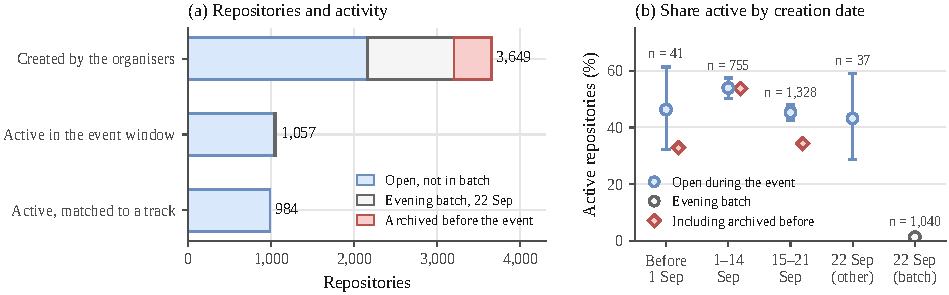
\includegraphics[width=\linewidth]{fig_population.pdf}
  \caption{Population. (a) Repositories created by the organisers, split into those open during the event and not in the evening batch, the batch, and those archived before the event; below them, the active repositories (the \NRqOneBatchActiveN{} of the batch form the thin grey segment) and those matched to a track. (b) Share of repositories that became active by creation date, with 95\% Wilson intervals, for repositories open during the event (circles; $n$ counts them) and for all repositories including those archived before the event (diamonds, without intervals, shown only where repositories of the group were archived before the event). The two repositories created on the event day are omitted.}
  \label{fig:population}
\end{figure}

\subsection{Work over the event window (RQ2)}\label{sec:process}

Active repositories received \NRqTwoWindowCommits{} team commits in the window. Activity rose during the first hour and stayed high through the afternoon, and the last hour held \NRqTwoLastHourSharePooled\% of all window commits, with the busiest ten minutes at \NRqTwoPeakOneZeroStart--\NRqTwoPeakOneZeroEnd{} (\cref{fig:process}a). The median team made \NRqTwoTeamShareMedian\% of its window commits in the last hour (IQR \NRqTwoTeamShareQOne--\NRqTwoTeamShareQThree\%), above the \evenshare{} of an even spread (\cref{fig:process}b). A minority of teams (\NRqTwoTeamsMajorityLastHourPct\%) made most of their commits in that hour, \NRqTwoTeamsAllLastHourN{} (\NRqTwoTeamsAllLastHourPct\%) made all of them in it, while \NRqTwoTeamsFourplusHoursPct\% committed in at least four of the five hours. Teams made their first window commit a median of \NRqTwoFirstCommitMinMedian{} minutes after the start (IQR \NRqTwoFirstCommitMinQOne--\NRqTwoFirstCommitMinQThree) and their last a median of \NRqTwoLastCommitMinBeforeDeadlineMedian{} minutes before the deadline, and made a median of \NRqTwoCommitsPerTeamMedian{} window commits (IQR \NRqTwoCommitsPerTeamQOne--\NRqTwoCommitsPerTeamQThree). Some active repositories also had commits from before the event (\NRqTwoPreEventRepos) or after the deadline (\NRqTwoPostDeadlineRepos).

In an exploratory analysis, $k$-means with two clusters on the teams' hourly profiles separated a late group of \NRqTwoClustersExploratoryLateN{} teams. The silhouette was \NRqTwoClustersExploratorySilhouette{}, above the mean silhouette of \NRqTwoClustersExploratoryNullMean{} (95th percentile \NRqTwoClustersExploratoryNullPNineFive) in \nullruns{} simulations without team structure~\cite{rousseeuw1987silhouettes}, but the two groups differed mainly in their last-hour share, which varies continuously across teams (\cref{fig:process}b). We therefore describe the distribution and do not assign teams to types: most worked through the afternoon with a moderate rise towards the deadline, and a minority left most of their commits to the last hour.

\begin{figure}[t]
  \centering
  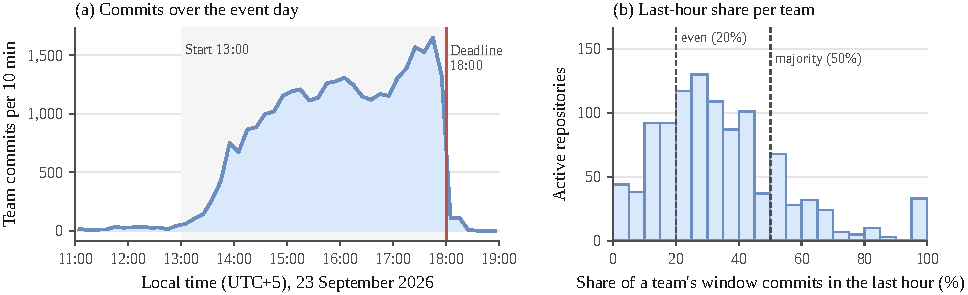
\includegraphics[width=\linewidth]{fig_process.pdf}
  \caption{Work over the event day. (a) Team commits per ten minutes, all branches of all repositories; the shaded band is the event window. (b) Distribution over the active repositories of the last-hour share $s_i$, in bins of five percentage points; the last bin holds the teams that made all their window commits in the last hour. Dashed lines mark an even spread (\evenshare) and a majority (\majorityshare).}
  \label{fig:process}
\end{figure}

\subsection{Traces of coding agents (RQ2)}\label{sec:traces}

Traces specific to Codex, the required tool, appeared in \NRqTwoTracesCodexSpecificN{} active repositories (\NRqTwoTracesCodexSpecificPct\%; \cref{fig:traces}a). Most were branches whose names start with \texttt{codex} (\NRqTwoTracesCodexBranchN{} of the \NRqTwoTracesCodexSpecificN; \NRqTwoTracesCodexBranchPct\% of active repositories), while authors named ``Codex'' (\NRqTwoTracesCodexNamePct\%) and commit signatures (\NRqTwoTracesCodexSignaturePct\%) were rare. An \texttt{AGENTS.md} file appeared in \NRqTwoTracesCodexFilePct\% of active repositories and was the only Codex-related trace in \NRqTwoTracesCodexFileOnlyN{} of them; counting it raises the share with a Codex trace to \NRqTwoTracesCodexAnyPct\%. The file was present in \NRqTwoTracesAgentsMdWithClaudePct\% of the repositories with a Claude Code trace, against \NRqTwoTracesAgentsMdWithoutClaudePct\% of the others. Claude Code, which was not required, left a trace in \NRqTwoTracesClaudeAnyPct\% of active repositories, mainly through signed commits (\NRqTwoTracesClaudeSignaturePct\%) and \texttt{CLAUDE.md} files (\NRqTwoTracesClaudeFilePct\%), and \NRqTwoTracesClaudeNotCodexSpecificPct\% had a Claude Code trace but no trace specific to Codex. Other agents appeared in few repositories (Cursor \NRqTwoTracesCursorAnyN, Copilot \NRqTwoTracesCopilotAnyN, Gemini \NRqTwoTracesGeminiAnyN), and \NRqTwoTracesNoTracePct\% of active repositories carried no trace of any agent.

At the level of commits, \NRqTwoTracesSignedCommitsPct\% of window commits carried an agent signature or an author named after a tool; \NRqTwoTracesSignedCommitsClaudeShare\% of these named Claude, and of the \NRqTwoTracesSignedCommitsByKindCodex{} that named Codex, \NRqTwoTracesSignedCommitsCodexNamedOnly{} did so only through the author name. Pull-request references, a workflow trace, occurred in \NRqTwoTracesPrRefsPct\% of active repositories.

In an analysis added after the plan, we compared the traces with what teams wrote in their README (\cref{fig:traces}b). Codex was named in the prose of \NRqTwoTracesSelfReportCodexStrictMentionN{} written READMEs (\NRqTwoTracesSelfReportCodexStrictMentionPct\% of written READMEs), and Claude Code in \NRqTwoTracesSelfReportClaudeStrictMentionN{} (\NRqTwoTracesSelfReportClaudeStrictMentionPct\%). Among the repositories that named Codex, \NRqTwoTracesSelfReportCodexStrictSpecificGivenMentionPct\% (95\% CI \NRqTwoTracesSelfReportCodexStrictSpecificGivenMentionLo--\NRqTwoTracesSelfReportCodexStrictSpecificGivenMentionHi) carried a trace specific to Codex and \NRqTwoTracesSelfReportCodexStrictAnyGivenMentionPct\% any Codex trace including \texttt{AGENTS.md}. A signature revealed Codex in \NRqTwoTracesSelfReportCodexStrictSignatureGivenMentionPct\% of them. Among the repositories that named Claude Code, \NRqTwoTracesSelfReportClaudeStrictAnyGivenMentionPct\% carried a Claude Code trace and \NRqTwoTracesSelfReportClaudeStrictSignatureGivenMentionPct\% a signature. Naming a tool and having any of its traces go together (odds ratio \NRqTwoTracesSelfReportCodexStrictAssocOr, 95\% CI \NRqTwoTracesSelfReportCodexStrictAssocLo--\NRqTwoTracesSelfReportCodexStrictAssocHi, for Codex including \texttt{AGENTS.md}, and \NRqTwoTracesSelfReportClaudeStrictAssocOr, \NRqTwoTracesSelfReportClaudeStrictAssocLo--\NRqTwoTracesSelfReportClaudeStrictAssocHi, for Claude Code, over the active repositories, with those without a written README counted as not naming the tool), so these shares describe detection among teams that name the tool, not the recall of the traces over all users. The broad definition gives the same contrast: a signature revealed Claude in \NRqTwoTracesSelfReportClaudeBroadSignatureGivenMentionPct\% of READMEs that contained the word and Codex in \NRqTwoTracesSelfReportCodexBroadSignatureGivenMentionPct\%.

\begin{figure}[t]
  \centering
  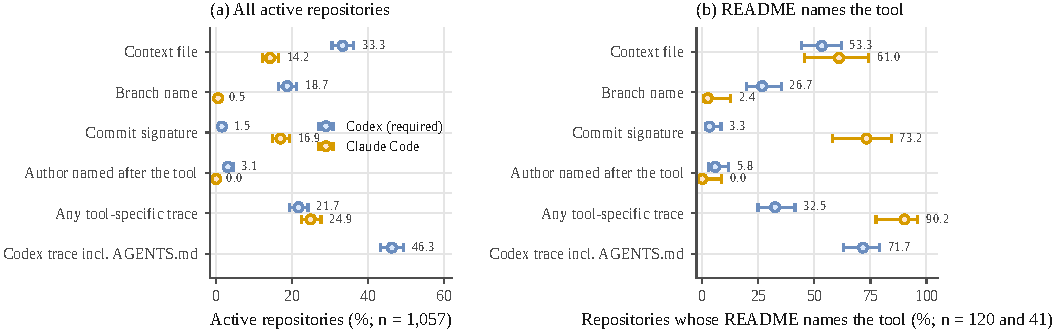
\includegraphics[width=\linewidth]{fig_traces.pdf}
  \caption{Traces of coding agents. (a) Share of active repositories with each kind of trace, for Codex, which every team had to use, and for Claude Code; for Codex the context file is the shared \texttt{AGENTS.md}, which the tool-specific trace excludes, and the last row adds it. That row is not shown for Claude Code, for which it equals the row above. (b) The same traces among the repositories whose README names the tool in its prose. Points are shares with 95\% Wilson intervals.}
  \label{fig:traces}
\end{figure}

Two further comparisons were exploratory. Agent-signed window commits were not consistently larger than other commits in the same repositories. In the \NRqTwoTracesCommitSizeAllRepos{} active repositories with both kinds, the per-repository median of signed commits was larger in \NRqTwoTracesCommitSizeAllSignedLargerPct\% of repositories (Wilcoxon $p$~\NRqTwoTracesCommitSizeAllP), but not among the \NRqTwoTracesCommitSizeMinThreeRepos{} repositories with at least three signed commits (\NRqTwoTracesCommitSizeMinThreeSignedLargerPct\%, $p$~\NRqTwoTracesCommitSizeMinThreeP) or for Claude-signed commits alone ($p$~\NRqTwoTracesCommitSizeClaudeP). Pooled over all signed and all other commits of these \NRqTwoTracesCommitSizePooledRepos{} repositories, the median changes were \NRqTwoTracesCommitSizePooledSigned{} and \NRqTwoTracesCommitSizePooledUnsigned{} lines. Signed commits more often had conventional-commit subjects (\NRqTwoTracesConventionalSignedPct\% of signed and \NRqTwoTracesConventionalUnsignedPct\% of other non-merge window commits).

In the planned comparison, repositories with an \texttt{AGENTS.md} file had more window commits (median \NRqTwoTracesAgentsMdAssocCommitsWith{} vs.\ \NRqTwoTracesAgentsMdAssocCommitsWithout; $\delta = \NRqTwoTracesAgentsMdAssocCommitsDelta$, Holm-adjusted $p$~\NRqTwoTracesAgentsMdAssocCommitsP), more hours with commits ($\delta = \NRqTwoTracesAgentsMdAssocHoursDelta$, $p$~\NRqTwoTracesAgentsMdAssocHoursP) and more often test files (\NRqTwoTracesAgentsMdAssocTestsWith\% vs.\ \NRqTwoTracesAgentsMdAssocTestsWithout\%, $V = \NRqTwoTracesAgentsMdAssocTestsV$, $p$~\NRqTwoTracesAgentsMdAssocTestsP), also after adjusting for the logarithm of one plus the number of window commits (odds ratio \NRqTwoTracesAgentsMdAssocTestsAdjustedOr, 95\% CI \NRqTwoTracesAgentsMdAssocTestsAdjustedLo--\NRqTwoTracesAgentsMdAssocTestsAdjustedHi). Teams that work through agents may produce both the file and the tests, and teams that prepared more may differ in other ways, so these are associations only.

\subsection{What teams built and documented (RQ3)}\label{sec:product}

Python was the primary language of \NRqThreePrimaryLanguagePythonPct\% of active repositories, followed by TypeScript (\NRqThreePrimaryLanguageTypeScriptPct\%) and JavaScript (\NRqThreePrimaryLanguageJavaScriptPct\%). React (\NRqThreeFrameworksReactPct\%) was the most common front-end framework and FastAPI (\NRqThreeFrameworksFastAPIPct\%) the most common back-end framework, with its server Uvicorn in \NRqThreeFrameworksUvicornPct\%; pytest appeared in \NRqThreeFrameworksPytestPct\%. An LLM SDK or API call appeared in \NRqThreeAnyLlmPct\% of repositories, OpenAI's in \NRqThreeLlmProvidersOpenAIPct\% and each other provider's in at most \NRqThreeLlmProvidersAnthropicPct\%. Test files were present in \NRqThreeTestsPct\% of repositories, and, by a stricter measure added after the plan, \NRqThreeTestFunctionsPct\% had a test file that defined at least one test; a Dockerfile in \NRqThreeDockerfilePct\%, a continuous-integration workflow in \NRqThreeCiPct\% and a deployment configuration in \NRqThreeDeployConfigPct\% (\cref{fig:product}). These shares hardly change when repositories with commits before the event or after the deadline are left out (test files \NRqThreeSensitivityNoPrePostTests\%).

\begin{figure}[t]
  \centering
  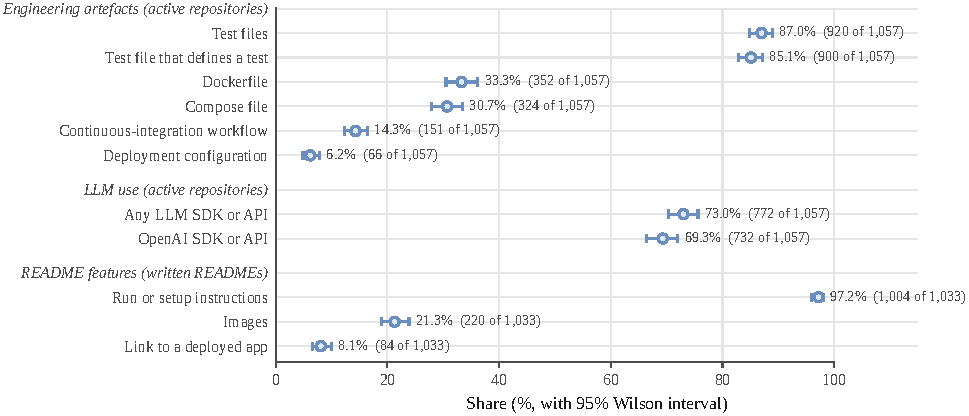
\includegraphics[width=\linewidth]{fig_product.pdf}
  \caption{What teams built. Engineering artefacts and LLM use in the \NRqOneActiveN{} active repositories, and README features in the \NRqThreeReadmeWritten{} of them with a written README; shares with 95\% Wilson intervals.}
  \label{fig:product}
\end{figure}

Most written READMEs were in Russian (\NRqThreeReadmeRussianPct\%), with English second (\NRqThreeReadmeEnglishPct\%) and Kazakh third (\NRqThreeReadmeKazakhPct\%), although Kazakh-specific letters appeared somewhere in \NRqThreeReadmeAnyKazakhLetterPct\%. Commit subjects, by contrast, were mostly in Latin script (\NRqThreeSubjectScriptLatinPct\% of non-merge window commits). The median README had \NRqThreeReadmeWordsMedian{} words (IQR \NRqThreeReadmeWordsQOne--\NRqThreeReadmeWordsQThree) and \NRqThreeReadmeHeadingsMedian{} headings; \NRqThreeReadmeRunInstructionsPct\% of READMEs gave run or setup instructions, \NRqThreeReadmeImagesPct\% included images and \NRqThreeReadmeDeployedLinkPct\% linked to a deployed application. The primary language (Python, TypeScript, JavaScript or other) differed between tracks (\cref{tab:tracks}; $\chisq(\NRqThreeLanguageByTrackDf) = \NRqThreeLanguageByTrackChiTwo$, $p$~\NRqThreeLanguageByTrackP, $V = \NRqThreeLanguageByTrackV$, with \NRqThreeLanguageByTrackCellsExpectedBelowFive{} of \NRqThreeLanguageByTrackCells{} cells having expected counts below five), from \NRqThreeTracksTOneTwoPython\% Python in the city-simulator track to \NRqThreeTracksTZeroFourPython\% in the telecom track. Window commits per team varied little between tracks ($H(\NRqThreeCommitsByTrackDf) = \NRqThreeCommitsByTrackH$, $p$~\NRqThreeCommitsByTrackP, $\epsq = \NRqThreeCommitsByTrackEpsTwo$). Kazakh READMEs were rare in every track, including the one whose task was to take minutes from Kazakh, Russian or mixed meeting audio (\NRqThreeTracksTZeroEightKazakh\%).

\begin{table}[t]
  \centering\small
  \caption{The \NTracksCount{} tracks with the active repositories matched to each, their median number of window commits, and the shares with test files, with Python as primary language and with a Kazakh README (of written READMEs). Partners are named in team READMEs; the briefs are summarised from those READMEs.}
  \label{tab:tracks}
  \begin{tabularx}{\linewidth}{@{}lll>{\raggedright\arraybackslash}Xrrrrr@{}}
    \toprule
    & Track & Partner & Brief & Repos & Commits & Tests & Python & Kazakh \\
    & & & & & (median) & (\%) & (\%) & (\%) \\
    \midrule
    T1 & Energy & Samruk-Kazyna & Agent that forecasts wind-farm output from weather data & \NRqThreeTracksTZeroOneN & \NRqThreeTracksTZeroOneCommits & \NRqThreeTracksTZeroOneTests & \NRqThreeTracksTZeroOnePython & \NRqThreeTracksTZeroOneKazakh \\
    T2 & Finance & Freedom & Rebuild an organised group from a transaction network & \NRqThreeTracksTZeroTwoN & \NRqThreeTracksTZeroTwoCommits & \NRqThreeTracksTZeroTwoTests & \NRqThreeTracksTZeroTwoPython & \NRqThreeTracksTZeroTwoKazakh \\
    T3 & Management & Halyk Bank & Guide linking employee skills to growth steps & \NRqThreeTracksTZeroThreeN & \NRqThreeTracksTZeroThreeCommits & \NRqThreeTracksTZeroThreeTests & \NRqThreeTracksTZeroThreePython & \NRqThreeTracksTZeroThreeKazakh \\
    T4 & Telecom & Beeline & Agent choosing tariff offers for subscribers & \NRqThreeTracksTZeroFourN & \NRqThreeTracksTZeroFourCommits & \NRqThreeTracksTZeroFourTests & \NRqThreeTracksTZeroFourPython & \NRqThreeTracksTZeroFourKazakh \\
    T5 & Logistics & ekt.kz & Supplier orders to replenish stock, approved by a manager & \NRqThreeTracksTZeroFiveN & \NRqThreeTracksTZeroFiveCommits & \NRqThreeTracksTZeroFiveTests & \NRqThreeTracksTZeroFivePython & \NRqThreeTracksTZeroFiveKazakh \\
    T6 & Creative industries & Firebird & Choose event contractors and explain the choice & \NRqThreeTracksTZeroSixN & \NRqThreeTracksTZeroSixCommits & \NRqThreeTracksTZeroSixTests & \NRqThreeTracksTZeroSixPython & \NRqThreeTracksTZeroSixKazakh \\
    T7 & Education & AI Sana & Turn a business problem into a task for student teams & \NRqThreeTracksTZeroSevenN & \NRqThreeTracksTZeroSevenCommits & \NRqThreeTracksTZeroSevenTests & \NRqThreeTracksTZeroSevenPython & \NRqThreeTracksTZeroSevenKazakh \\
    T8 & Innovation & Samruk-Kazyna & Minutes and action items from Kazakh, Russian or mixed meeting audio & \NRqThreeTracksTZeroEightN & \NRqThreeTracksTZeroEightCommits & \NRqThreeTracksTZeroEightTests & \NRqThreeTracksTZeroEightPython & \NRqThreeTracksTZeroEightKazakh \\
    T9 & Communications & Halyk Bank & Voice agent that routes calls in an insurance contact centre & \NRqThreeTracksTZeroNineN & \NRqThreeTracksTZeroNineCommits & \NRqThreeTracksTZeroNineTests & \NRqThreeTracksTZeroNinePython & \NRqThreeTracksTZeroNineKazakh \\
    T10 & Trade & ekt.kz & Shopping assistant: products, alternatives, prices, stock & \NRqThreeTracksTOneZeroN & \NRqThreeTracksTOneZeroCommits & \NRqThreeTracksTOneZeroTests & \NRqThreeTracksTOneZeroPython & \NRqThreeTracksTOneZeroKazakh \\
    T11 & Special (structure) & Kazakhtelecom & Compare organisation charts before and after a reorganisation & \NRqThreeTracksTOneOneN & \NRqThreeTracksTOneOneCommits & \NRqThreeTracksTOneOneTests & \NRqThreeTracksTOneOnePython & \NRqThreeTracksTOneOneKazakh \\
    T12 & Special (city) & Astana Innovations & City simulator that splits a budget across districts & \NRqThreeTracksTOneTwoN & \NRqThreeTracksTOneTwoCommits & \NRqThreeTracksTOneTwoTests & \NRqThreeTracksTOneTwoPython & \NRqThreeTracksTOneTwoKazakh \\
    \bottomrule
  \end{tabularx}
\end{table}

\subsection{How teams solved the same brief (RQ3)}\label{sec:approach}

In exploratory analyses added after the plan, solutions to the same brief were more alike than solutions to different briefs. The mean Jaccard similarity of the dependency sets was \NRqThreeSolutionsDepsWithin{} for pairs of repositories with the same track and \NRqThreeSolutionsDepsAcross{} for pairs with different tracks (permutation $p$~\NRqThreeSolutionsDepsP, the smallest value that \solruns{} shuffles allow), and most briefs had their own distinctive libraries (\cref{tab:approach}), such as NetworkX for the transaction network, faster-whisper and pyannote.audio for the meeting minutes and scikit-learn for the wind forecast. The excess similarity did not differ clearly between pairs in which both repositories had agent traces (\NRqThreeSolutionsDepsWithExcess) and pairs in which neither did (\NRqThreeSolutionsDepsWithoutExcess; $p$~\NRqThreeSolutionsDepsStatusP). File paths and README headings were also more alike within briefs, though less than dependencies (\NRqThreeSolutionsPathsRatio{} and \NRqThreeSolutionsHeadingsRatio{} times the cross-brief similarity, against \NRqThreeSolutionsDepsRatio{} for dependencies), and for file paths the excess similarity was smaller for pairs with agent traces (\NRqThreeSolutionsPathsWithExcess{} against \NRqThreeSolutionsPathsWithoutExcess; $p$~\NRqThreeSolutionsPathsStatusP), a difference we did not examine further. Of the source files that occurred unchanged in more than one repository, \NRqThreeSolutionsSharedFilesSeveralTracks{} appeared in several tracks and were mostly generated scaffolding of web frameworks, and \NRqThreeSolutionsSharedFilesOneTrack{} were confined to one track. The most widely shared of the one-track files were starter code supplied with the finance, telecom and call-routing briefs, and most of the rest belonged to one third-party agent skill found in two repositories of the contractor track; beyond these, identical files gave no sign that teams copied each other's code.

The coded approaches show the same pattern. The core method differed strongly between briefs ($\chisq(\NRqThreeApproachByTrackDf) = \NRqThreeApproachByTrackChiTwo$, $p$~\NRqThreeApproachByTrackP, $V = \NRqThreeApproachByTrackV$; \NRqThreeApproachByTrackCellsExpectedBelowFive{} of \NRqThreeApproachByTrackCells{} cells had expected counts below five, \NRqThreeApproachSmallCellsRare{} of them for the rare pretrained and unclear codes), and in \NRqThreeApproachBriefsTopSevenFive{} of the \NTracksCount{} briefs one core method was used by at least three quarters of the teams. Most teams used rules or an algorithm for the transaction-network, skills-guide, tariff, replenishment, contractor and budget briefs, a trained model for the wind forecast, and an LLM for briefs built around dialogue or documents, such as task cards, shopping assistance and call routing. Across all briefs, \NRqThreeApproachPatternExplainsPct\% of teams let rules or a trained model do the task and used an LLM only to explain or present the result, \NRqThreeApproachPatternLlmTaskPct\% let an LLM produce the main result, \NRqThreeApproachPatternNoLlmPct\% used no LLM, and \NRqThreeApproachPatternOtherPct\% fitted none of these patterns. Nearly all teams built a web application (\NRqThreeApproachWebAppPct\%), and \NRqThreeApproachEvaluationPct\% of READMEs reported a measured result of the solution.

\begin{table}[t]
  \centering\small
  \caption{How teams solved each brief. Main method: the most common core method in the coded approaches and the share of the track's teams that used it; effective number: the exponential of the Shannon entropy of the method shares; LLM result: teams whose LLM produces the main result; distinctive libraries: the two dependencies most over-represented in the track, among those used by at least a quarter of its teams and at least twice as often as in other tracks, with the share that used them (a dash where none qualifies).}
  \label{tab:approach}
  \begin{tabularx}{\linewidth}{@{}ll>{\raggedright\arraybackslash}Xrrr>{\raggedright\arraybackslash}X@{}}
    \toprule
    & Track & Main method & Share (\%) & Eff.\ number & LLM result (\%) & Distinctive libraries \\
    \midrule
    T1 & Energy & \NRqThreeApproachTracksTZeroOneTopMethod & \NRqThreeApproachTracksTZeroOneTopShare & \NRqThreeApproachTracksTZeroOneEffectiveMethods & \NRqThreeApproachTracksTZeroOneLlmTaskPct & \NRqThreeApproachTracksTZeroOneLibraries \\
    T2 & Finance & \NRqThreeApproachTracksTZeroTwoTopMethod & \NRqThreeApproachTracksTZeroTwoTopShare & \NRqThreeApproachTracksTZeroTwoEffectiveMethods & \NRqThreeApproachTracksTZeroTwoLlmTaskPct & \NRqThreeApproachTracksTZeroTwoLibraries \\
    T3 & Management & \NRqThreeApproachTracksTZeroThreeTopMethod & \NRqThreeApproachTracksTZeroThreeTopShare & \NRqThreeApproachTracksTZeroThreeEffectiveMethods & \NRqThreeApproachTracksTZeroThreeLlmTaskPct & \NRqThreeApproachTracksTZeroThreeLibraries \\
    T4 & Telecom & \NRqThreeApproachTracksTZeroFourTopMethod & \NRqThreeApproachTracksTZeroFourTopShare & \NRqThreeApproachTracksTZeroFourEffectiveMethods & \NRqThreeApproachTracksTZeroFourLlmTaskPct & \NRqThreeApproachTracksTZeroFourLibraries \\
    T5 & Logistics & \NRqThreeApproachTracksTZeroFiveTopMethod & \NRqThreeApproachTracksTZeroFiveTopShare & \NRqThreeApproachTracksTZeroFiveEffectiveMethods & \NRqThreeApproachTracksTZeroFiveLlmTaskPct & \NRqThreeApproachTracksTZeroFiveLibraries \\
    T6 & Creative industries & \NRqThreeApproachTracksTZeroSixTopMethod & \NRqThreeApproachTracksTZeroSixTopShare & \NRqThreeApproachTracksTZeroSixEffectiveMethods & \NRqThreeApproachTracksTZeroSixLlmTaskPct & \NRqThreeApproachTracksTZeroSixLibraries \\
    T7 & Education & \NRqThreeApproachTracksTZeroSevenTopMethod & \NRqThreeApproachTracksTZeroSevenTopShare & \NRqThreeApproachTracksTZeroSevenEffectiveMethods & \NRqThreeApproachTracksTZeroSevenLlmTaskPct & \NRqThreeApproachTracksTZeroSevenLibraries \\
    T8 & Innovation & \NRqThreeApproachTracksTZeroEightTopMethod & \NRqThreeApproachTracksTZeroEightTopShare & \NRqThreeApproachTracksTZeroEightEffectiveMethods & \NRqThreeApproachTracksTZeroEightLlmTaskPct & \NRqThreeApproachTracksTZeroEightLibraries \\
    T9 & Communications & \NRqThreeApproachTracksTZeroNineTopMethod & \NRqThreeApproachTracksTZeroNineTopShare & \NRqThreeApproachTracksTZeroNineEffectiveMethods & \NRqThreeApproachTracksTZeroNineLlmTaskPct & \NRqThreeApproachTracksTZeroNineLibraries \\
    T10 & Trade & \NRqThreeApproachTracksTOneZeroTopMethod & \NRqThreeApproachTracksTOneZeroTopShare & \NRqThreeApproachTracksTOneZeroEffectiveMethods & \NRqThreeApproachTracksTOneZeroLlmTaskPct & \NRqThreeApproachTracksTOneZeroLibraries \\
    T11 & Special (structure) & \NRqThreeApproachTracksTOneOneTopMethod & \NRqThreeApproachTracksTOneOneTopShare & \NRqThreeApproachTracksTOneOneEffectiveMethods & \NRqThreeApproachTracksTOneOneLlmTaskPct & \NRqThreeApproachTracksTOneOneLibraries \\
    T12 & Special (city) & \NRqThreeApproachTracksTOneTwoTopMethod & \NRqThreeApproachTracksTOneTwoTopShare & \NRqThreeApproachTracksTOneTwoEffectiveMethods & \NRqThreeApproachTracksTOneTwoLlmTaskPct & \NRqThreeApproachTracksTOneTwoLibraries \\
    \bottomrule
  \end{tabularx}
\end{table}

\subsection{Credential exposure (RQ4)}\label{sec:exposure}

Gitleaks' generic rule produced \NRqFourGenericFindings{} findings in \NRqFourGenericRepos{} repositories, \NRqFourGenericDataFilesPct\% of them in data files (\texttt{.json}, \texttt{.jsonl}, \texttt{.txt} or \texttt{.csv}); we treat these as low-precision and do not analyse them further. Format-specific rules produced \NRqFourProviderFindings{} findings, of which \NRqFourProviderPlaceholder{} were placeholders. The other \NRqFourProviderPlausible{} lie in \NRqFourReposProviderN{} active repositories (\NRqFourReposProviderPct\%), and in \NRqFourReposProviderFinalN{} repositories (\NRqFourReposProviderFinalPct\% of the active ones) a string matched by the same rule is still present in the same file in the final version (\cref{fig:risk}a). Most match the OpenAI API key format: \NRqFourOpenaiFindings{} findings in \NRqFourOpenaiN{} repositories (\NRqFourOpenaiPct\%), \NRqFourOpenaiFinalN{} of which still hold such a string. By the author dates that Gitleaks reports, all OpenAI key strings were committed during the event window.

\begin{figure}[t]
  \centering
  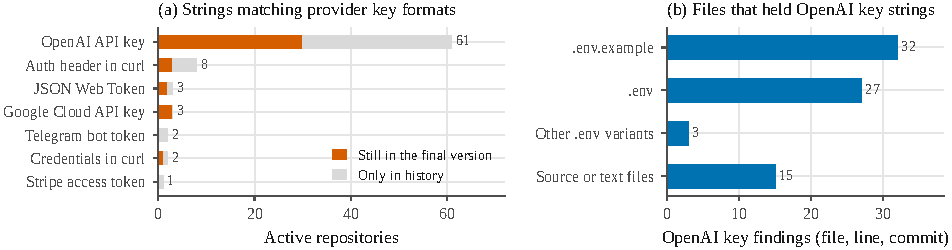
\includegraphics[width=\linewidth]{fig_risk.pdf}
  \caption{Credential exposure. (a) Active repositories with strings matched by the format-specific rules of Gitleaks, split by whether a string matched by the same rule is still present in the same file in the final version. A repository can appear in more than one row. (b) Files that held the OpenAI key strings; a finding is one file, line and commit, so a key can be counted more than once.}
  \label{fig:risk}
\end{figure}

The OpenAI key strings sat mainly in environment files (\cref{fig:risk}b): \NRqFourOpenaiFilesEnvExample{} findings in \texttt{.env.example} and \NRqFourOpenaiFilesEnv{} in \texttt{.env}. A \texttt{.env.example} file is a template meant to be committed, so a real key placed there becomes public even when \texttt{.gitignore} excludes \texttt{.env}. In the final state, \texttt{.gitignore} covered \texttt{.env} in \NRqFourGitignoreCoversEnvPct\% of active repositories and a \texttt{.env.example} file was present in \NRqFourEnvExamplePct\%. In an exploratory analysis, key strings were not clearly more frequent where the final \texttt{.gitignore} covered \texttt{.env} (\NRqFourGitignoreAssocWithIgnore\% vs.\ \NRqFourGitignoreAssocWithoutIgnore\%, $V = \NRqFourGitignoreAssocV$, $p$~\NRqFourGitignoreAssocP). Coverage went with LLM use (\NRqFourGitignoreAssocIgnoreAmongLlm\% of repositories with an LLM SDK against \NRqFourGitignoreAssocIgnoreAmongNoLlm\% without), and adjusting for LLM use gave a Mantel--Haenszel odds ratio of \NRqFourGitignoreAssocMhOr{} (95\% CI \NRqFourGitignoreAssocMhLo--\NRqFourGitignoreAssocMhHi, $p$~\NRqFourGitignoreAssocMhP). Of the \NRqFourKeyCommitsFindings{} OpenAI findings, \NRqFourKeyCommitsMatched{} could be matched to a commit on a branch, and \NRqFourKeyCommitsSignedN{} of these (\NRqFourKeyCommitsSignedPct\%) carried an agent signature, against \NRqFourKeyCommitsBaselineSignedSameReposPct\% of all window commits in the same repositories. Because Codex signatures were rare, this does not show that agents were uninvolved.

% =====================================================================================
\section{Discussion}\label{sec:discussion}

\subsection{Denominators decide rates}
The same event yields an activity rate of \NRqOneActivePct\%, \NRqOneActiveOfOpenPct\% or \NRqOneActiveOfOpenNonbatchPct\%, depending on whether the repositories closed by the organisers and the batch created the evening before are counted. Taken over all repositories, the data suggest that the date of registration mattered a great deal ($\chisq(\NRqOneCreationChiTwoAllDf) = \NRqOneCreationChiTwoAllChiTwo$, $p$~\NRqOneCreationChiTwoAllP, $V = \NRqOneCreationChiTwoAllV$, with the batch counted with \batchday), whereas among open repositories outside the batch the effect is small ($V = \NRqOneCreationChiTwoOpenNonbatchV$). We do not know why the organisers archived repositories in bulk or created the batch; the allocation of limited seats, which the news reports describe~\cite{qumash2026queue,ulys2026survival}, and withdrawn or duplicate registrations are possible reasons. Archived repositories also held work from before the event about five times as often as open ones, which fits both teams that tried their repository early and then withdrew and the removal of repositories in which work had started early. Organiser-created repositories record the organisers' actions as well as the teams', so archive times, creation bursts and template commits have to be reconstructed before any rate is read as participation. Datasets built from project listings face the opposite problem, since they never contain the empty repositories~\cite{imam2021secretlife,mahmoud2022oneoff}.

\subsection{What traces reveal when the tool is known}
Every team was told to use Codex, yet traces specific to Codex appeared in about a fifth of the active repositories, and Codex-related traces of any kind in fewer than half, even counting \texttt{AGENTS.md}. These data cannot separate compliance from detection, because the observed share is the product of the two; even if every team used Codex, the traces recovered that use in at most \NRqTwoTracesCodexAnyPct\% of the active repositories. Because Codex was required and reads \texttt{AGENTS.md}, we take this share as the closer estimate of Codex-related traces, and the \NRqTwoTracesCodexSpecificPct\% with traces specific to Codex as a lower bound that does not depend on who wrote the file. Detection also differed sharply between tools. Claude Code adds a co-author trailer to its commits by default~\cite{claudecode2026attribution}; we found no documented default for Codex, whose signatures were rare here even among teams that named it (\cref{tab:estimates}). Adoption estimates that rest mainly on commit signatures may therefore count tools that sign by default more completely than tools that do not; running each tool with its default settings in a test repository would check this mechanism directly. The comparison among teams that name each tool also sets two unlike groups side by side. Codex was required, so naming it may state compliance, whereas naming Claude Code was voluntary and may come from heavy users, whose README the agent may have written. The gap in any tool-specific trace (\NRqTwoTracesSelfReportClaudeStrictSpecificGivenMentionPct\% against \NRqTwoTracesSelfReportCodexStrictSpecificGivenMentionPct\%) is smaller than the gap in signatures, but it mixes the same two effects. Estimates that combine several traces~\cite{robbes2026agenticmuch} depend less on one tool's defaults, but they too cannot see use that leaves no trace. Robbes et al.\ discuss the pitfalls of detecting agents from traces~\cite{robbes2026heuristics}; a known required tool shows how large the gap can be in one setting.

We could not confirm that agent-signed commits are larger than other commits, as Robbes et al.\ found at scale~\cite{robbes2026agenticmuch}: the difference depended on which repositories were included. The Claude Code traces also give a lower bound on the use of a tool that the rules did not require. The rules named Codex, and whether they excluded other tools is not stated in the sources we read, so we do not treat these traces as breaches.

\subsection{Work, artefacts and language}
Deadline pressure was visible but moderate. The median team made \NRqTwoTeamShareMedian\% of its window commits in the last hour, more than an even spread would give, and most teams committed in at least four of the five hours. Studies of time pressure mostly report higher productivity and lower quality~\cite{kuutila2020timepressure}, and in programming courses students who start late tend to score lower~\cite{edwards2009behaviors,kazerouni2017procrastination}. Whether the teams that left most of their work to the last hour built weaker prototypes is one of the questions of the pre-registered analysis of the jury's decisions.

Test files, long READMEs with run instructions and, in a third of repositories, Dockerfiles were produced within five hours. One explanation, which our data cannot test, is that agents make such artefacts cheap to produce, since in many real agent sessions the agent writes nearly all of the committed code~\cite{baumann2026swechat}. The quality risks of agent-written code are documented elsewhere~\cite{he2026cursor,zhao2025vibesafe,deng2026vibeinsecurity}. Teams given the same brief also converged on similar solutions, and their library overlap was not clearly greater among teams that left agent traces. A common design let rules or a trained model do the task and an LLM explain the result, which fits briefs that ask for decisions that can be checked. Whether this convergence came from the briefs themselves or from similar tools answering the same brief, we cannot say. The documentation was written mostly in Russian, and Kazakh was rare even in the track built around Kazakh audio. Language models still score lower on Kazakh-language benchmarks than on benchmarks in high-resource languages~\cite{togmanov2025kazmmlu}, which may make teams less inclined to work with agents in Kazakh, but the audience that teams wrote for may matter as much, and our data cannot separate the two.

\subsection{Implications}
For organisers, creating repositories after check-in would turn the GitHub organisation into a record of participants rather than of registrations. Because many of the exposed keys sat in \texttt{.env.example}, a file meant to be committed, simple measures could have closed this route. GitHub blocks pushes of OpenAI API keys to public repositories by default, but the block can be bypassed~\cite{github2026pushprotection,github2026patterns}, and we cannot tell whether the strings found here were pushed past it, pushed while it did not apply, or were not live keys. Repository templates that ship a \texttt{.gitignore} and a placeholder-only \texttt{.env.example}, push protection at the level of the organisation, which is off by default and turns bypasses into alerts~\cite{github2026pushprotection}, and short-lived keys issued for the event would all help, in line with earlier recommendations~\cite{meli2019git,krause2022pushed}. For researchers who measure agent use from repositories, our results suggest reporting how the population was formed, separating traces that are specific to one tool from files that several tools may read, reporting each trace for each tool, and checking trace-based estimates, where possible, against a reference such as a known required tool or what developers state.

% =====================================================================================
\section{Threats to validity}\label{sec:threats}

We organise the threats following the empirical standards for repository mining~\cite{ralph2020standards}.

\paragraph{Construct validity.} Author identities overstate the number of people. Commit counts measure activity, not effort or quality, and test files show an intention to test, not working tests. Agent traces are partial by design. \texttt{AGENTS.md} is read by several agents, and an author named ``Codex'' is a trace whose origin we could not verify. Naming a tool in a README does not show how much the tool was used, and it means different things for a required and a voluntary tool. We therefore report what each kind of trace shows and treat none of them as a measure of use. The README language rule is a letter heuristic that misses Kazakh typed with Russian or Latin letters, and its errors lay mainly in READMEs it called Kazakh or mixed (\cref{sec:validation}), so the Kazakh share may be slightly overstated. The coded approaches rest on what the README states and on one hosted model at one date, and they were not checked against hand labels; the dependency sets rest on declared manifests. Credential findings match key formats, were not tested, and depend on a placeholder filter that was not validated against hand labels.

\paragraph{Internal validity and reliability.} The event window is inferred rather than taken from a schedule, but it is supported by the archive times, and shifting it changes the number of active repositories little (\cref{tab:validation}). Features are measured at the final state, which in some repositories includes commits from before the event or after the deadline; leaving those repositories out barely changes the shares. The \texttt{.gitignore} rules are also measured at the final state, not at the time a key was committed. Reading bulk archiving from last-update times is an inference, consistent with the absence of any commit in those repositories during the event. The associations with \texttt{AGENTS.md} and \texttt{.gitignore} are observational, and the README-naming and commit-size analyses were added after the analysis plan. Track labels come from keyword rules on README text, so teams that did not describe their task stay unassigned, and the labels and the README language sample were checked by one person. The default-branch commit at which each clone ended is released, so that the data can be collected again.

\paragraph{External validity.} We study one in-person event in one country, with one required agent and a five-hour window. Other events differ in duration, rules, tools and participants, the default behaviour of agents changes between versions, and the share of empty repositories depends on how an organiser provisions them.

% =====================================================================================
\section{Conclusions}\label{sec:conclusion}

A hackathon at which the organisers created the repositories and fixed the tool allows repository measures to be checked against what was known in advance. At HackAlem AI, the choice of denominator moved the activity rate by \NRqOneActiveGapPp{} percentage points, because the organisers archived repositories and created a batch before the event. Traces specific to the required agent appeared in about a fifth of the active repositories, and Codex-related traces of any kind in fewer than half, even counting \texttt{AGENTS.md}, which several agents read. In an exploratory comparison among teams that named each tool, signatures revealed Claude Code, which was not required and signs its commits by default, far more often than Codex. Teams given the same brief used more similar libraries and, by the coded approaches, mostly one kind of method; their library overlap was not clearly greater among teams that left agent traces. OpenAI key strings became public mainly through committed \texttt{.env.example} and \texttt{.env} files. Studies of AI coding agents that start from repositories should therefore report how their population was formed and what each trace can recover. Several questions remain open. After the awards, we will test the pre-registered hypotheses about the jury's decisions and compare these repositories with hackathon repositories from before coding agents~\cite{halmans2026hackrep}. Running each agent with its default settings would show which traces it leaves; running the teams' tests and hand-labelling a sample of approaches would check the test files and the coded approaches.

% =====================================================================================
\section*{Author contributions}
Talgar Bayan conceived and designed the study, collected and analysed the data, and wrote and revised the paper.

\section*{Funding}
This research received no external funding.

\section*{Institutional review board statement}
Not applicable. The study used only public repositories and public web pages, involved no interaction with human participants, and accessed no private system. Personal data and credentials were handled as described in \cref{sec:credentials}, and the organisers were informed of the exposed credentials before publication.

\section*{Informed consent statement}
Not applicable.

\section*{Data availability statement}
The pseudonymised dataset, the pipeline, the analysis plan and its deviations are available at \url{https://github.com/tbayan/HackalemAI-Repo-Data-Mining} and archived on Zenodo as release \zenodoversion{} (\zenodorelease). The released data use random identifiers; because the source repositories are public, this is pseudonymisation and not anonymisation. Credential findings are released only as aggregates. The analysis of the jury's decisions was pre-registered on the Open Science Framework before any finalist or winner was announced (\url{https://osf.io/bm3je}), following a template for secondary data analysis~\cite{vandenakker2021prereg}.

\section*{Conflicts of interest}
The author declares no conflicts of interest. The author is not affiliated with the organisers of HackAlem AI, and this paper reports no official results of the event.

\section*{Abbreviations}
API, application programming interface; CI, confidence interval; IQR, interquartile range; LLM, large language model; SDK, software development kit.

\bibliographystyle{unsrtnat}
\bibliography{references}

\end{document}
